%% History:
% Pavel Tvrdik (26.12.2004)
%  + initial version for PhD Report
% Daniel Sykora (27.01.2005)
% Michal Valenta (3.12.2008)
% rada zmen ve formatovani (diky M. Duškovi, J. Holubovi a J. Žďárkovi)
% sjednoceni zdrojoveho kodu pro anglickou, ceskou, bakalarskou a diplomovou praci

% One-page layout: (proof-)reading on display
%%%% \documentclass[11pt,oneside,a4paper]{book}
% Two-page layout: final printing
\documentclass[11pt,twoside,a4paper]{book}   
%=-=-=-=-=-=-=-=-=-=-=-=--=%
% The user of this template may find useful to have an alternative to these 
% officially suggested packages:
\usepackage[czech, english]{babel}
\usepackage[T1]{fontenc} % pouzije EC fonty 
% pripadne pisete-li cesky, pak lze zkusit take:
\usepackage[OT1]{fontenc} 
\usepackage[utf8]{inputenc}
\usepackage{lmodern}
%=-=-=-=-=-=-=-=-=-=-=-=--=
%=-=-=-=-=-=-=-=-=-=-=-=--=%
% Depending on your particular TeX distribution and version of conversion tools 
% (dvips/dvipdf/ps2pdf), some (advanced | desperate) users may prefer to use 
% different settings.
% Please uncomment the following style and use your CSLaTeX (cslatex/pdfcslatex) 
% to process your work. Note however, this file is in UTF-8 and a conversion to 
% your native encoding may be required. Some settings below depend on babel 
% macros and should also be modified. See \selectlanguage \iflanguage.
%\usepackage{czech}  %%%%%\usepackage[T1]{czech} %%%%[IL2] [T1] [OT1]
%=-=-=-=-=-=-=-=-=-=-=-=--=%

%%%%%%%%%%%%%%%%%%%%%%%%%%%%%%%%%%%%%%%
% Styles required in your work follow %
%%%%%%%%%%%%%%%%%%%%%%%%%%%%%%%%%%%%%%%
\usepackage{graphicx}
\usepackage{indentfirst} %1. odstavec jako v cestine.

\usepackage{k336_thesis_macros} % specialni makra pro formatovani DP a BP
 % muzete si vytvorit i sva vlastni v souboru k336_thesis_macros.sty
 % najdete  radu jednoduchych definic, ktere zde ani nejsou pouzity
 % napriklad: 
 % \newcommand{\bfig}{\begin{figure}\begin{center}}
 % \newcommand{\efig}{\end{center}\end{figure}}
 % umoznuje pouzit prikaz \bfig namisto \begin{figure}\begin{center} atd.
 
%jaa

\usepackage{float}

\usepackage{listings}
\usepackage{courier}
\lstset{
	language=Java,
	basicstyle=\footnotesize\ttfamily,
	commentstyle=\color{gray},
	keywordstyle=\color{blue},
	stringstyle=\color{BurntOrange},
	numbers=left,
	numberstyle=\tiny\ttfamily,
	%stepnumber=2,
	numbersep=5pt,
	tabsize=2,
	showstringspaces=false,
	extendedchars=true,
	breaklines=true,
	frame=b,
	xleftmargin=17pt,
	framexleftmargin=17pt,
	framexrightmargin=5pt,
	framexbottommargin=4pt,
}
\renewcommand*\lstlistingname{Zdrojový kód}
\usepackage{color}
\usepackage[usenames,dvipsnames]{xcolor}
\usepackage{caption}
\DeclareCaptionFont{white}{\color{white}}
\DeclareCaptionFormat{listing}{\colorbox{gray}{\parbox{\textwidth}{#1#2#3}}}
\captionsetup[lstlisting]{format=listing,labelfont=white,textfont=white}


\newcommand\TypeOfWork{Bakalářská práce}  \typeout{Bakalarska prace}
\newcommand\StudProgram{Softwarové technologie a management, Bakalářský}
\newcommand\StudBranch{Web a multimedia}                  % pro STM

\newcommand\WorkTitle{Planární segmentace mračna bodů}
\newcommand\FirstandFamilyName{Daniel Princ}
\newcommand\Supervisor{Ing. David Sedláček}


% Pouzijete-li pdflatex, tak je prijemne, kdyz bude mit vase prace funkcni odkazy i v pdf formatu
\usepackage[
pdftitle={\WorkTitle},
pdfauthor={\FirstandFamilyName},
bookmarks=true,
colorlinks=true,
breaklinks=true,
urlcolor=red,
citecolor=blue,
linkcolor=blue,
unicode=true,
]
{hyperref}


% Extension posted by Petr Dlouhy in order for better sources reference (\cite{} command) especially in Czech.
% April 2010
% See comment over \thebibliography command for details.
\usepackage[square, numbers]{natbib}             % sazba pouzite literatury
%\usepackage{url}
%\DeclareUrlCommand\url{\def\UrlLeft{<}\def\UrlRight{>}\urlstyle{tt}}  %rm/sf/tt
%\renewcommand{\emph}[1]{\textsl{#1}}    % melo by byt kurziva nebo sklonene,
\let\oldUrl\url
\renewcommand\url[1]{<\texttt{\oldUrl{#1}}>}


\begin{document}
\selectlanguage{czech}
% prikaz \typeout vypise vyse uvedena nastaveni v prikazovem okne
% pro pohodlne ladeni prace
 \typeout{************************************************}
 \typeout{Zvoleny jazyk: cestina}
 \typeout{Typ prace: \TypeOfWork}
 \typeout{Studijni program: \StudProgram}
 \typeout{Obor: \StudBranch}
 \typeout{Jmeno: \FirstandFamilyName}
 \typeout{Nazev prace: \WorkTitle}
 \typeout{Vedouci prace: \Supervisor}
 \typeout{***************************************************}
 \newcommand\Department{Katedra počítačové grafiky a interakce}
 \newcommand\Faculty{Fakulta elektrotechnická}
 \newcommand\University{České vysoké učení technické v Praze}
 \newcommand\labelSupervisor{Vedoucí práce}
 \newcommand\labelStudProgram{Studijní program}
 \newcommand\labelStudBranch{Obor}


%%%%%%%%%%%%%%%%%%%%%%%%%%    Poznamky ke kompletaci prace
% Nasledujici pasaz uzavrenou v {} ve sve praci samozrejme 
% zakomentujte nebo odstrante. 
% Ve vysledne svazane praci bude nahrazena skutecnym 
% oficialnim zadanim vasi prace.
%{
%\pagenumbering{roman}\setcounter{page}{1}\cleardoublepage \thispagestyle{empty}
%\chapter*{Na tomto místě bude oficiální zadání vaší práce}
%\begin{itemize}
%\item Toto zadání je podepsané děkanem a vedoucím katedry,
%\item musíte si ho vyzvednout na studijním oddělení Katedry počítačů na Karlově náměstí,
%\item v jedné odevzdané práci bude originál tohoto zadání (originál zůstává po obhajobě na katedře),
%\item ve druhé bude na stejném místě neověřená kopie tohoto dokumentu (tato se vám vrátí po obhajobě).
%\end{itemize}
%\newpage
%}

%%%%%%%%%%%%%%%%%%%%%%%%%%    Titulni stranka / Title page 
\coverpagestarts

%%%%%%%%%%%%%%%%%%%%%%%%%%%    Podekovani / Acknowledgements 
\acknowledgements
\noindent
Chtěl bych poděkovat vedoucímu této práce, panu Ing. Davidovi Sedláčkovi, za poskytnutí cenných rad a nápadů.


%%%%%%%%%%%%%%%%%%%%%%%%%%%   Prohlaseni / Declaration 
\declaration{V~Praze dne 24.\,5.\,2015}


%%%%%%%%%%%%%%%%%%%%%%%%%%%%    Abstract 
\abstractpage
This bachelor's thesis concerns about point cloud processing, specifically about planar segmentation of point clouds. Planar segmentation finds its use in 3D digital reconstruction of objects from the real world. Currently, there has been significant interest to automate the process of data reconstruction, planar segmentation is one of the basic parts of this process.

Specifically, the goal of this thesis is to implement an algorithm, that will perform the segmentation as automatically as possible and in sufficient quality. The algorithm is implemented as a part of reconstruction software ArchiRec3D.

% Prace v cestine musi krome abstraktu v anglictine obsahovat i
% abstrakt v cestine.
\vglue60mm

\noindent{\Huge \textbf{Abstrakt}}
\vskip 2.75\baselineskip

\noindent
Tato bakalářská práce se zabývá problematikou zpracování mračna bodů, konkrétně segmentací na planární
primitiva. Toto má uplatnění zejména při digitální 3D rekonstrukci objektů reálného světa. V současné době je
snaha co nejvíce automatizovat proces zpracování naměřených dat, planární segmentace je jednou ze základních
částí tohoto procesu.

Konkrétním cílem této bakalářské práce je implementovat algoritmus, který budou segmentaci provádět co
nejvíce automaticky a zároveň v dostatečné kvalitě. Algoritmus je implementován jako součást 3D
rekonstrukčního nástroje ArchiRec3D.

%%%%%%%%%%%%%%%%%%%%%%%%%%%%%%%%  Obsah / Table of Contents 
\tableofcontents

%%%%%%%%%%%%%%%%%%%%%%%%%%%%%%%  Seznam obrazku / List of Figures 
\listoffigures

%%%%%%%%%%%%%%%%%%%%%%%%%%%%%%%  Seznam tabulek / List of Tables
\listoftables

%**************************************************************

\mainbodystarts
% horizontalní mezera mezi dvema odstavci
%\parskip=5pt
\normalfont
\parskip=0.4\baselineskip plus 0.2\baselineskip minus 0.1\baselineskip

% Odsazeni prvniho radku odstavce resi class book (neaplikuje se na prvni 
% odstavce kapitol, sekci, podsekci atd.) Viz usepackage{indentfirst}.
% Chcete-li selektivne zamezit odsazeni 1. radku nektereho odstavce,
% pouzijte prikaz \noindent.

%**************************************************************

% Pro snadnejsi praci s vetsimi texty je rozumne tyto rozdelit
% do samostatnych souboru nejlepe dle kapitol a tyto potom vkladat
% pomoci prikazu \include{jmeno_souboru.tex} nebo \include{jmeno_souboru}.
% Napr.:
% \include{1_uvod}
% \include{2_teorie}
% atd...
%*****************************************************************************
\chapter{Úvod}
Rekonstrukce 3D modelů se dnes uplatňuje v mnoha oborech. Běžně se můžeme setkat např. s vizualizacemi, které
se často využívají pro simulaci vzhledu města při výstavbě nových objektů. V takovém případě se obvykle
naskenuje aktuální stav okolí výstavby, do kterého se přidá model plánované budovy. Výsledná vizualizace poté
umožňuje posoudit vliv nové výstavby v kontextu okolí. Výhoda je také v tom, že takovéto simulace snadno pochopí i
laický pozorovatel. Využití lze nalézt i v technické praxi, kde mohou 3D modely zachytit aktuální stav
zařízení (např. potrubí v elektrárně), které nemusí odpovídat zastaralé či nekompletní dokumentaci. Přesné 3D
modely krajiny se mohou využívat např. při modelování záplav nebo šíření bezdrátového signálu. Podobně se
modely mohou využívat k modelování šíření zvuku v uzavřených prostorech. Dále můžeme najít rozsáhlé využití v
archeologii a ochraně kulturního dědictví, v dokumentaci důlních děl, monitorování krajiny pro detekci
nebezpečných sesuvů, mapování pobřežních oblastí a mořského dna v okolí přístavů apod.

Existuje několik metod, které se ke sběru těchto dat využívají. Tradiční metodou je fotogrammetrie, kdy se
informace o objektu získávají z několika fotografií a pro případné zpřesnění se může využít geodetického
zaměření. Hlavní nevýhodou této metody je přesnost naměřených dat, která výrazně klesá se vzdáleností měření.
Tato metoda nám obvykle poskytuje souřadnice charakteristických bodů, jako jsou hrany, vrcholy apod. To může
být velká nevýhoda zejména u nepravidelných objektů.

Jednou z nejnovějších metod sběru dat je laserové skenování. Jeho hlavní výhodou je rychlý sběr velkého
množství přesných dat v terénu. Nevýhodou oproti předchozí metodě je zejména špatná identifikace hran a
vrcholů. Další nevýhodou může být fakt, že přístroje pro laserové skenování jsou velmi drahé. Slabinou této
metody je také náročné zpracování, které se neobejde bez výkonné výpočetní techniky. Základním výstupem z
laserového skenování je mračno bodů. Jedná se o tisíce až miliony bodů, které jsou definovány třemi
kartézskými souřadnicemi (x, y, z), dále mohou obsahovat informaci o barvě (r, g, b) a případně také normálu
(n$_x$, n$_y$, n$_z$) k ploše, na které se bod vyskytuje.

\section{Segmentace mračna bodů}

V této práci se zabývám zpracováním mračna bodů, konkrétně jeho planární segmentací. Cílem práce je tedy
identifikovat ve vstupním mračnu bodů rovinné útvary, přiřadit jednotlivé body do těchto rovinných útvarů a
případně zahodit body, které v žádné rovinně neleží (viz Obr. \ref{fig:ukazkova-scena}). Tato segmentace
má smysl zejména v architektuře a archeologii, tedy při rekonstrukci budov a podobných objektů, které jsou
složeny z relativně malého počtu velkých rovin (tedy stěny, střechy apod.).

\begin{figure}[ht]
\begin{center}
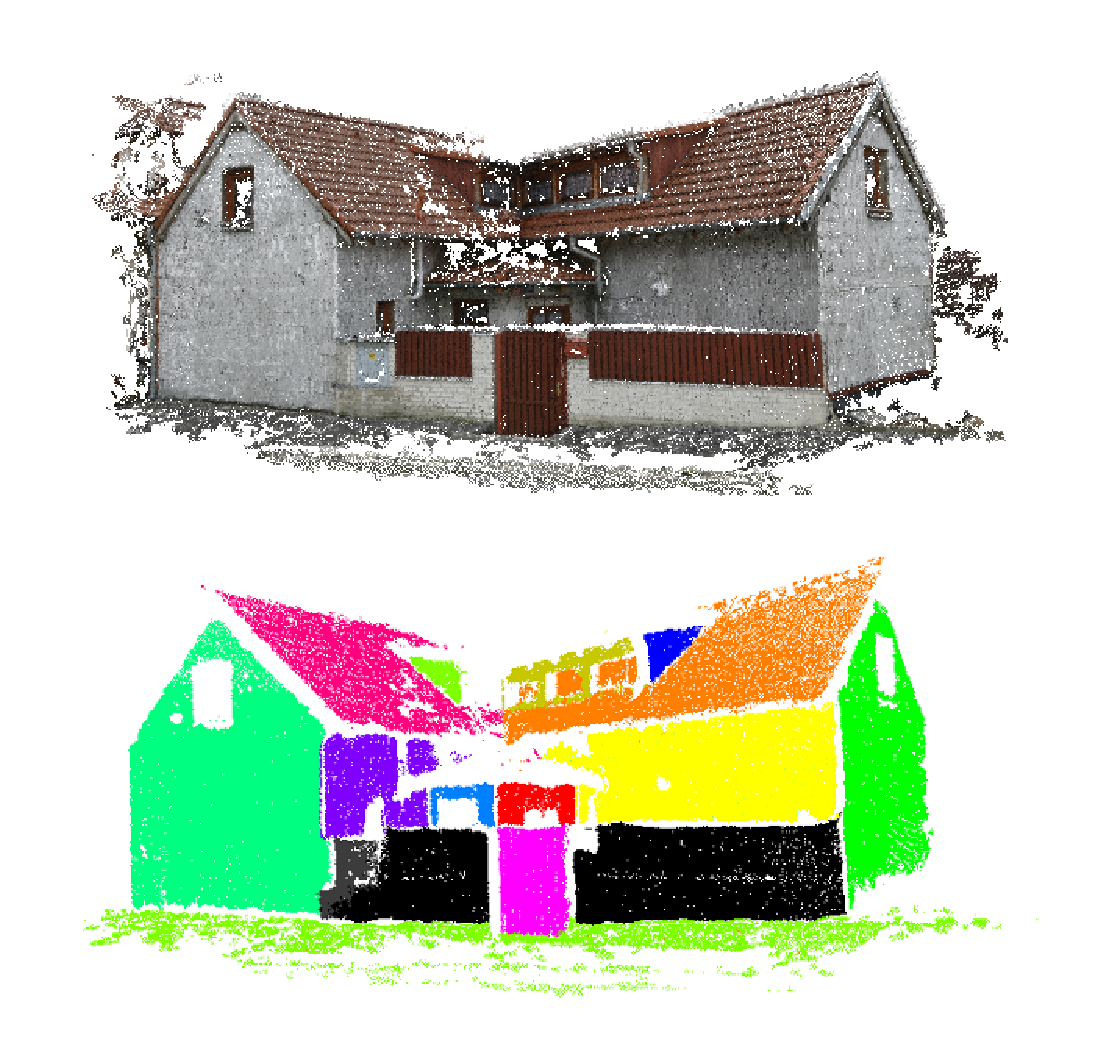
\includegraphics[height=10cm]{figures/ukazka-segmentace}
\caption{Ukázková scéna (nahoře) a její planární segmentace (dole).}
\label{fig:ukazkova-scena}
\end{center}
\end{figure}

Segmentační metody můžeme hrubě rozdělit do dvou základních kategorií \cite{Voss04}. Jednak jsou to metody, které segmentují na základě vlastností jako je vzdálenost bodů v prostoru a případně podobnost lokálně odhadnutých normál. Sem spadají např. metody, jako je segmentace na základě skenovacích linií\footnote{V anglické literatuře se označuje jako \uv{scan line segmentation} \cite{Voss04}} nebo surface growing. První zmíněná metoda vychází z toho, že data jsou pořizována postupně podél skenovacích linií. Body v těchto liniích jsou nejprve rozděleny do rovných přímek a poté jsou ve 3D prostoru na základě podobných atributů slučovány do jednotlivých segmentů. Surface growing algoritmy fungují tak, že je vybrán rovinný či nerovinný prvek (seed region) a ten je poté postupně spojován s blízkými body, které mají podobné atributy. Tato metoda je ale silně závislá na volbě vhodného původního prvku.

Do druhé kategorie spadají metody, které přímo odhadují parametry roviny na základě shlukování bodů a vyhledávání lokálních maxim v prostoru parametrů. Sem patří např. rozšíření Houghovi transformace pro 3D prostor. Jeden bod v mračnu, který se nachází na ploše v objektovém prostoru definuje rovinu v prostoru parametrů. Body na stejné ploše mají poté podobné parametry (vzdálenost od počátku a naklonění roviny) a na základě těchto parametrů jsou poté shlukovány. Jednotlivé shluky bodů pak podle dalších kritérií vytvoří jeden segment. Tato a další podobné metody mají zejména výpočetní problémy, protože mají velké paměťové nároky. Obvyklým problémem obou výše zmíněných kategorií je fakt, že jednotlivé metody se často zaměřují pouze na specifický typ vstupních dat (letecké skeny nebo pozemní skeny).

Článek \cite{Seg01} navrhuje řešení, které zohledňuje jak podobnost bodů v prostoru atributů, tak vzdálenost bodů v objektovém prostoru. Zároveň snižuje počet atributů pro vyšší efektivitu a menší paměťové nároky. Dále by také metoda neměla být závislá na typu vstupních dat.


\section{Struktura práce}

V této práci bych měl popsat a implementovat dva zadané algoritmy \cite{Seg01} a \cite{Seg02}. První algoritmus se ale v průběhu práce ukázal náročnější, než jsem předem očekával. Po dohodě s vedoucím práce je tedy v této práci popsán a implementován pouze tento první algoritmus.  

Práce nejprve v kapitole \ref{chap:analyza} popisuje zadaný algoritmus \cite{Seg01} a věnuje se návrhu jeho implementace. Poté následuje kapitola \ref{chap:implementace} popisující samotnou implementaci algoritmu. Algoritmus je implementován v rámci dodaného nástroje ArchiRec3D \cite{AR3D}, který je psaný v jazyku Java. V závěrečné části práce v kapitole \ref{chap:test} je otestována správná funkčnost algoritmu na uměle generovaných datech a na reálných datech je otestována kvalita algoritmu a jeho implementace. V závěru jsou shrnuty výsledky testování a analyzovány nedostatky algoritmu. Je zda také zhodnoceno, zda jsou nedostatky způsobeny návrhem algoritmu nebo jeho implementací.


%*****************************************************************************
%\chapter{Popis problému, specifikace cíle}

%\begin{itemize}
%\item Vysvětlení pojmů
%\item Popis řešeného problému, vymezení cílů DP/BP a požadavků na implementovaný systém.
%\item Popis struktury DP/BP ve vztahu k vytyčeným cílům.
%\item Rešeršní zpracování existujících implementací, pokud jsou známy.
%\end{itemize}

%*****************************************************************************
\chapter{Analýza a návrh řešení}
\label{chap:analyza}

\section{Segmentace na základě velikosti normálového vektoru}

Navržený proces segmentace v článku \cite{Seg01} zahrnuje tři hlavní kroky - definici okolí, výpočet atributů a klastrování bodů. Definice okolí bodu bere v úvahu 3D vzdálenost mezi body a tvar povrchu, na kterém se bod nachází. Parametry daného bodu jsou poté vypočteny na základě tohoto definovaného okolí. Pro nižší paměťové nároky jsou pro každý bod použity pouze dva parametry. Po vypočtení parametrů je provedeno klastrování bodů ležících ve stejné rovině, které zohledňuje jak podobnost v prostoru parametrů, tak vzdálenost bodů v prostoru.

\subsection{Adaptivní válcová definice okolí} 
\label{sub:def-okoli}

Správná definice okolí bodu je zásadní podmínkou pro správnou funkčnost algoritmu, protože okolí bodu přímo ovlivňuje parametry, které jsou pro daný bod vypočteny. V tomto algoritmu je okolí definováno tak, že bere v úvahu vzdálenost bodů v prostoru, ale zároveň také tvar povrchu, na kterém se bod nachází.

Proces definice okolí je znázorněn v diagramu na obrázku \ref{fig:diagram-okoli}. Cílem tohoto procesu je získat lokální okolí zkoumaného bodu, konkrétně blízké sousední body ležící ve stejné rovině. Na základě toho okolí jsou poté pro každý bod vypočteny parametry, které slouží pro následné klastrování bodů. Prvním krokem při definici okolí je vytvořit kouli se středem v bodu, pro který okolí definujeme. Poloměr koule volíme takový, aby obsahovala dostatečný počet bodů pro spolehlivý výpočet parametrů. Tuto hodnotu nejde přesněji specifikovat, musí být odvozena z konkrétního mračna bodů, které zpracováváme\footnote{Nicméně praxe ukazuje, že vhodná volba jsou řádově desítky až stovky bodů uvnitř koule.}. Poté vezmeme všechny body, které leží uvnitř této koule, a proložíme je pomocí metody nejmenších čtverců výchozí rovinou (viz Obr. \ref{fig:definice-okoli} (a)). Poté, co je rovina proložena, vypočítáme pro každý bod v kouli jeho vzdálenost od této roviny. Inverzi této vzdálenosti použijeme v další iteraci jako váhu bodu\footnote{Jednoduše řečeno, čím je bod od roviny dál, tím je jeho váha nižší.}, jak můžeme vidět v rovnici \ref{eq:vypocet-vahy}:

\begin{equation}
w_i = \frac{1}{d_i}
\label{eq:vypocet-vahy}
\end{equation}

\noindent
kde $w_i$ značí váhu i-tého bodu a  $d_i$ je vzdálenost bodu od proložené roviny. Tím jsme pro každý bod v okolí získali váhu. Nyní okolí znovu proložíme rovinou, ale vezmeme v úvahu vypočtené váhy. Tento proces \uv{převažování roviny} se iterativně opakuje, dokud se roviny v rámci iterací již nemění nebo dokud není dosaženo daného počtu iterací (např. 10). Poté je rovnoběžně nad a pod výslednou rovinou definován buffer. Velikost tohoto bufferu je závislá na očekávané velikosti šumu ve vstupních datech. Body, které jsou uvnitř tohoto bufferu, tvoří konečné okolí (viz Obr. \ref{fig:definice-okoli}(b)). Ostatní body mimo buffer se již na okolí nijak nepodílejí.

\begin{figure}[ht]
\begin{center}
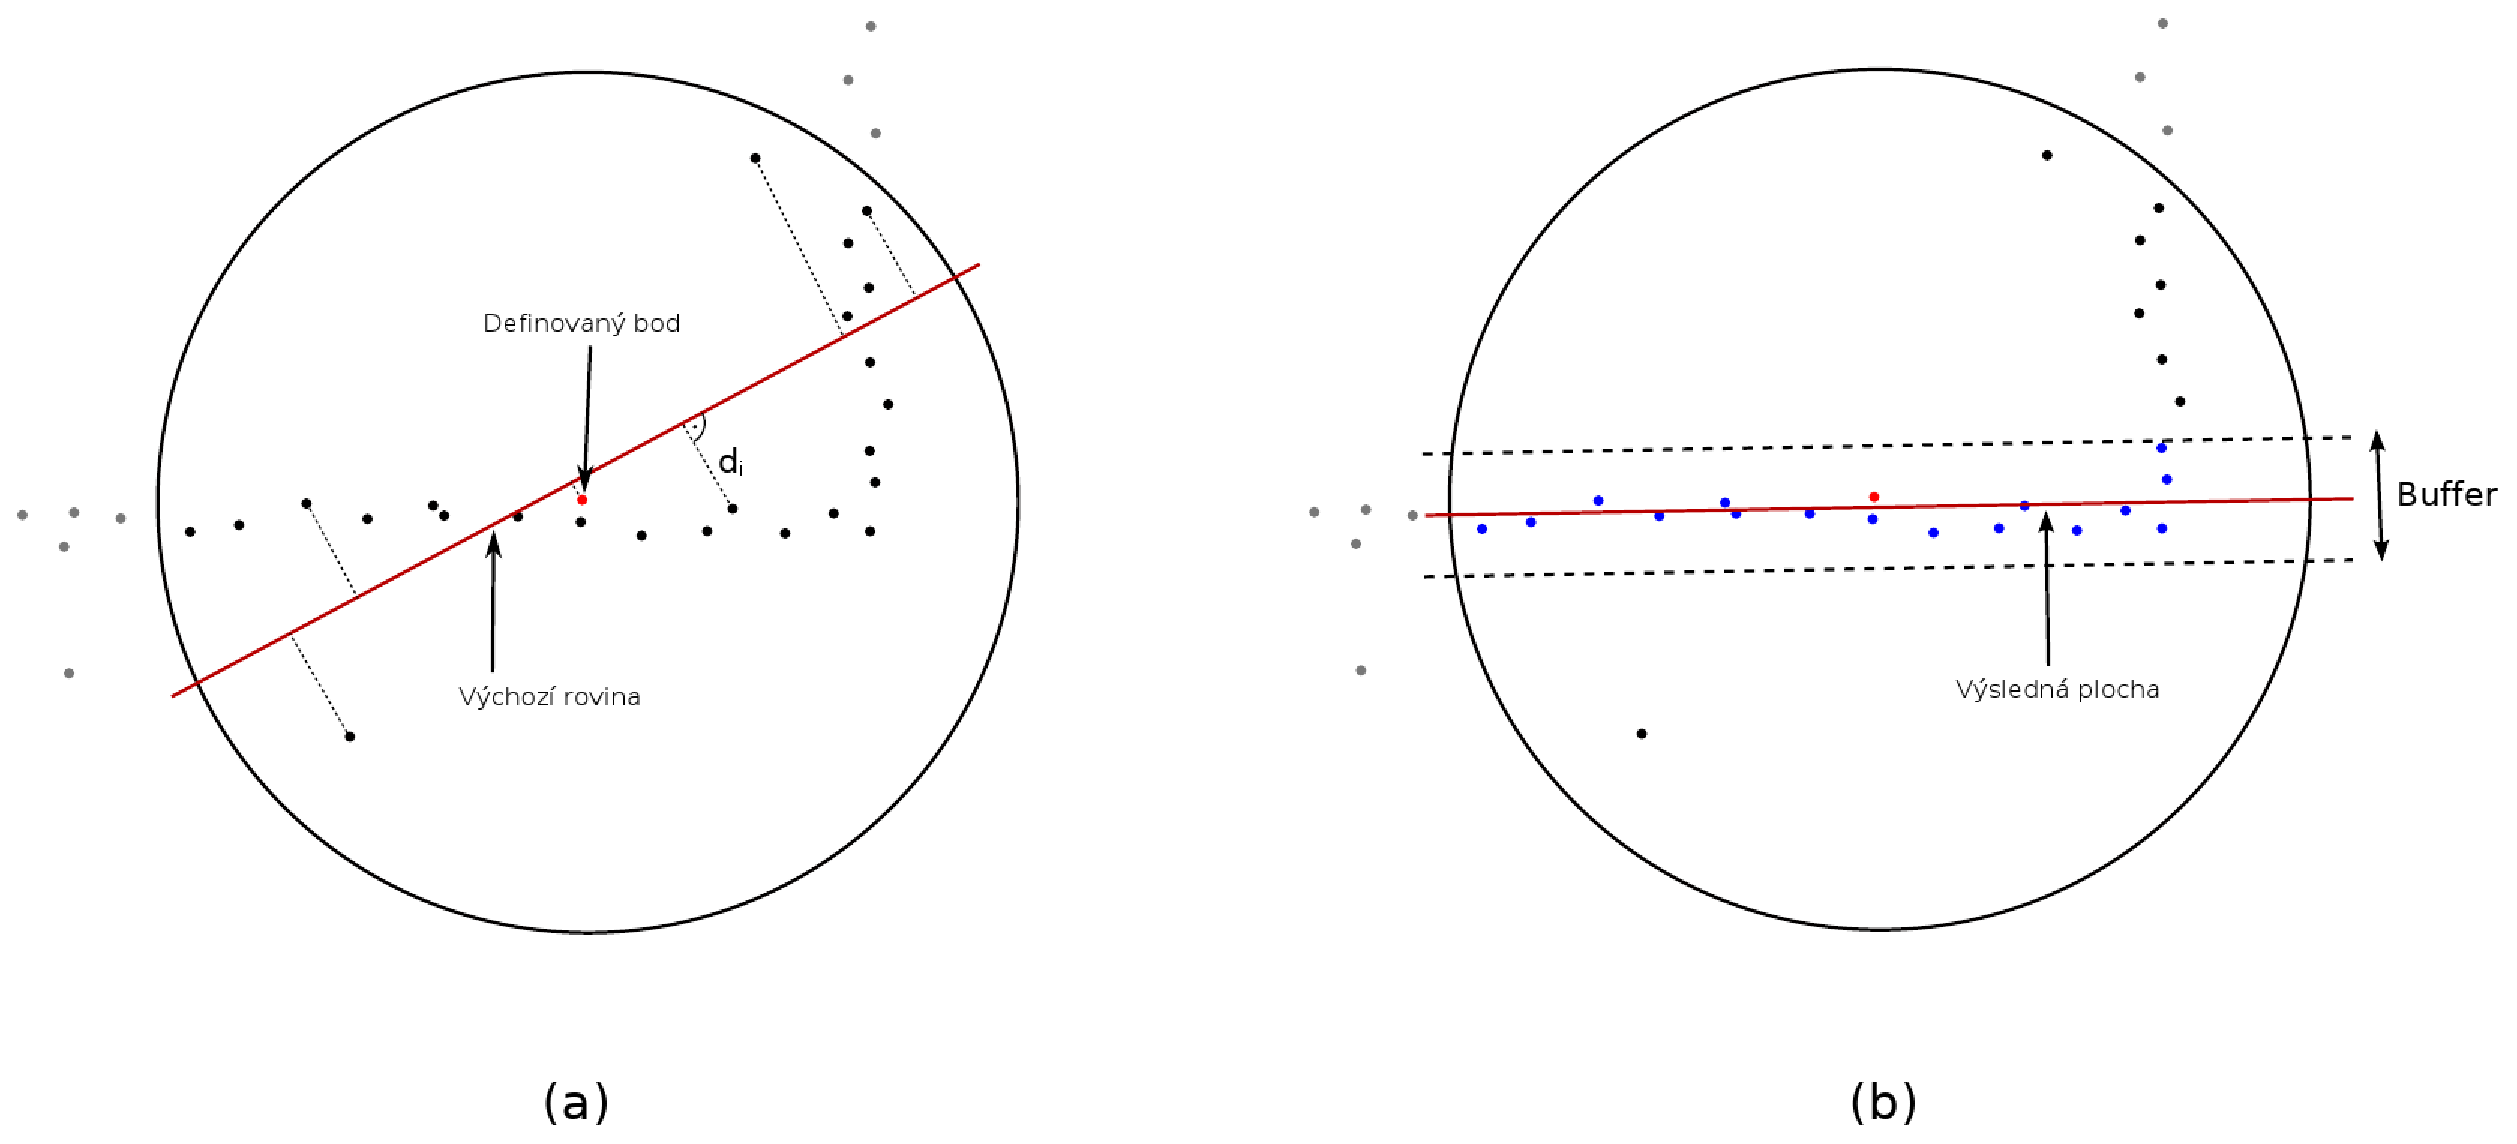
\includegraphics[width=\textwidth]{figures/definice-okoli}
\caption{Definice okolí bodu (boční pohled).\newline (a) zobrazuje proložení původní roviny body uvnitř koule. Pro některé body je znázorněna jejich vzdálenost od roviny $d_i$.\newline (b) znázorňuje výslednou rovinu po iterativním procesu, který zahrnuje váhy jednotlivých bodů. Okolí tvoří modře vyznačené body uvnitř bufferu.}
\label{fig:definice-okoli}
\end{center}
\end{figure}

Výsledné okolí se tedy nachází v útvaru, který téměř odpovídá nízkému válci, jehož osa je normála k ploše, na které se původní bod nachází. Tato osa navíc může být v průběhu algoritmu oproti výchozí hodnotě značně upravena, proto je tato metoda označena jako adaptivní válcová definice okolí. 

\begin{figure}[ht]
\begin{center}
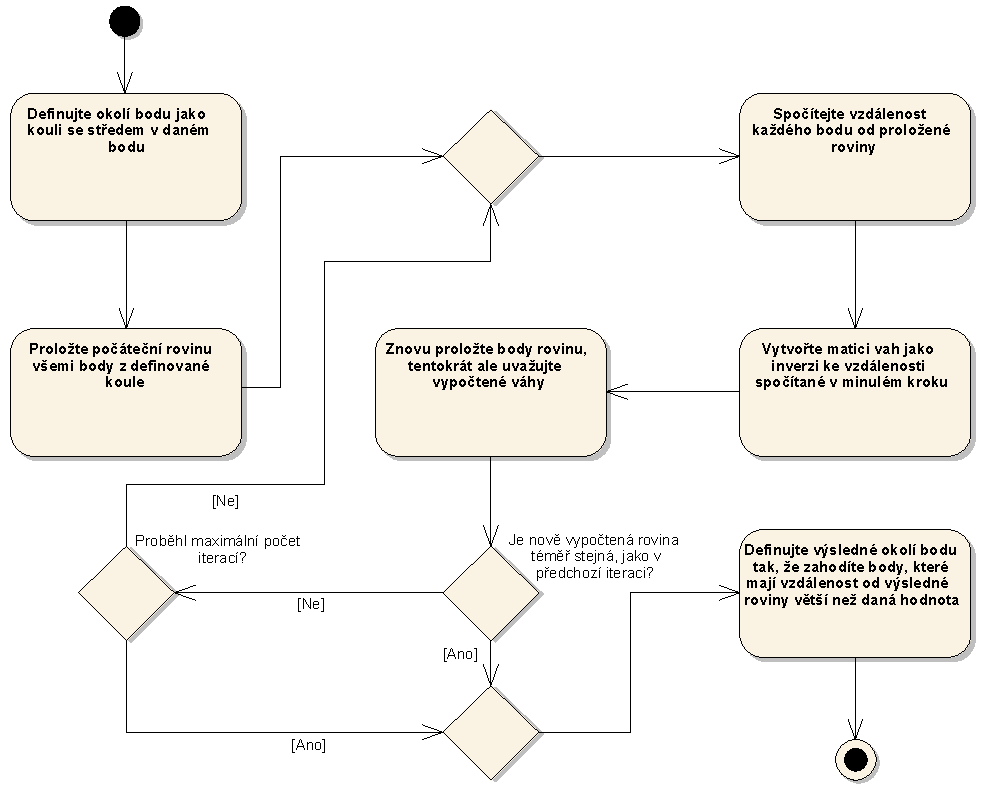
\includegraphics[width=\textwidth]{figures/okoli-diagram}
\caption{Diagram aktivit znázorňující proces definice okolí bodu.}
\label{fig:diagram-okoli}
\end{center}
\end{figure}

\newpage
\subsection{Výpočet parametrů bodu}

Parametry bodu jsou, jak již bylo zmíněno, vypočítány na základě okolí bodu. Pokud zavedeme do mračna bodů nějaký referenční bod, můžeme definovat normálový vektor z tohoto bodu na rovinu, na které se daný bod nachází. Většina metod, které provádějí klastrování na základě vypočtených parametrů, využívá hlasování do akumulátorového pole vytvořeného v prostoru parametrů. Akumulátorové pole je v podstatě čítač, který si při hlasování ukládá počet hlasů na dané pozici. To nám umožňuje rychle vyhledat, která pozice má největší počet hlasů. Rozměry akumulátorového pole závisí na počtu použitých parametrů. Můžeme tedy použít 3 složky normálového vektoru jako parametry a tím zajistíme, že všechny segmenty budou správně rozeznány\footnote{Mělo by být jasné, že jeden normálový vektor jednoznačně definuje rovinu.}. Nicméně takovýto způsob vyžaduje vytvoření třírozměrného akumulátorového pole a hlasování do 3D pole je výpočetně náročná operace. 

Pro snížení výpočetních nároků je tedy nutné snížit počet parametrů. Proto je jako atribut využita velikost normálového vektoru\footnote{Tedy jde o vzdálenost roviny od referenčního bodu.}. Toto řešení přináší ale nebezpečí v tom, že může existovat více rovin ve stejné vzdálenosti od referenčního bodu a v takovém případě by několik rovin splynulo do jednoho segmentu. Jako řešení je zaveden druhý referenční bod a tedy i druhý parametr. Tím se značně snižuje riziko situace, kdy by více rovin mělo stejnou vzdálenost od dvou různých bodů. Obrázek \ref{fig:normal-def} (a) schématicky znázorňuje situaci, kdy mají dvě roviny stejnou vzdálenost od jednoho bodu, ale různou vzdálenost od druhého bodu, každá rovina bude mít tedy jiný pár parametrů. Na obrázku \ref{fig:normal-def} (b) jsou znázorněny hlasy jednotlivých rovin zaznamenané v akumulátorovém poli. Všechny body jsou v poli zaznamenány na základě těchto dvou vypočtených parametrů. Body, které patří do různých rovin, jsou tedy v akumulátorovém poli umístěné na různých místech. Hlavní výhodou tohoto řešení je tedy to, že jsme snížili počet parametrů definujících rovinu a tím také ubrali jeden rozměr akumulátorového pole.

\begin{figure}[ht]
\begin{center}
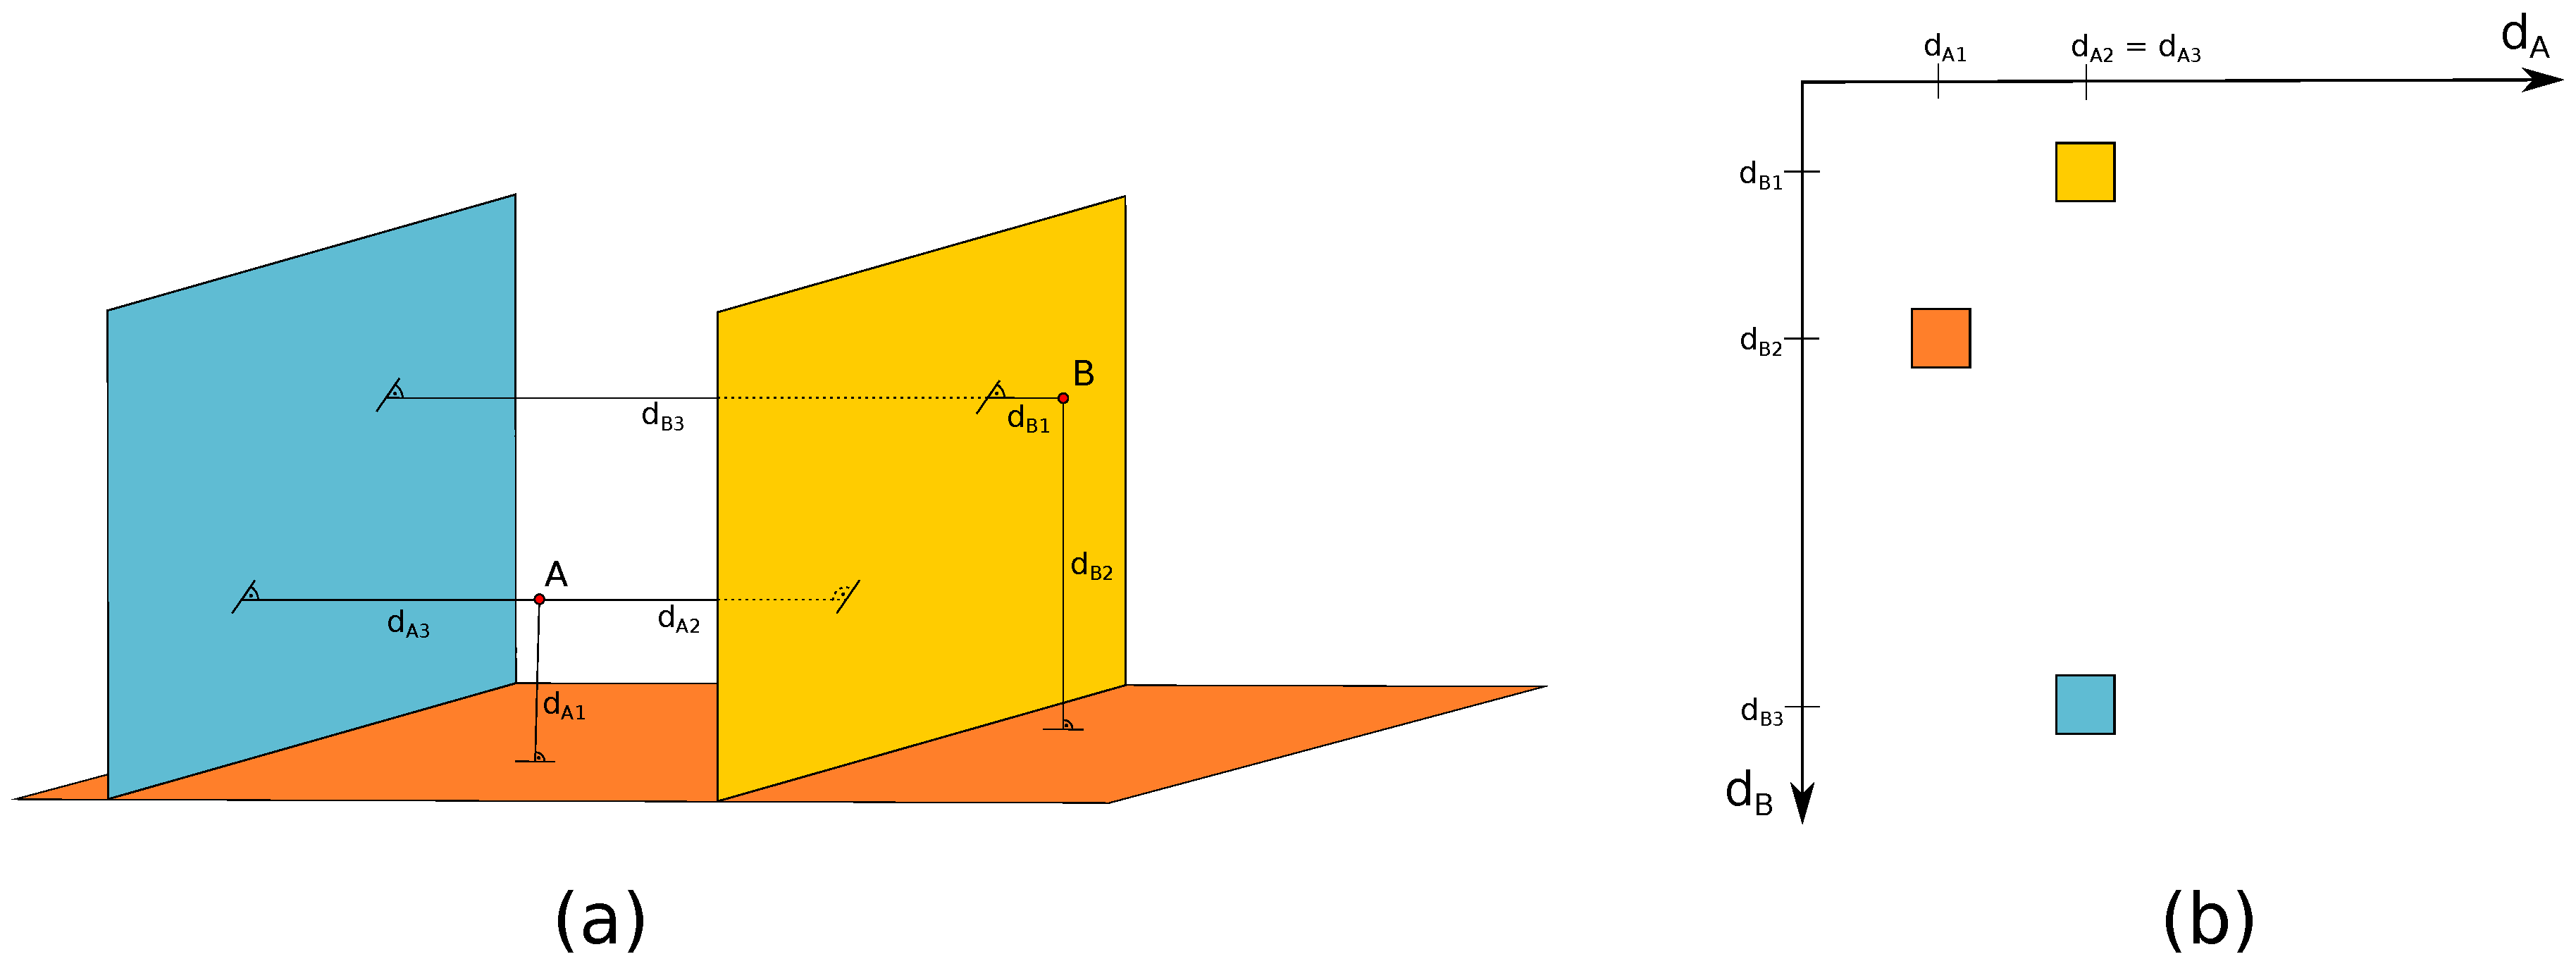
\includegraphics[width=\textwidth]{figures/definice-normal}
\caption{Schématické znázornění situace, kdy jsou dvě roviny stejně vzdálené od bodu A, ale různě vzdálené od bodu B (a), zaznamenané hlasy v akumulátorovém poli (b). Vzdálenost roviny od bodu A je značena jako $d_A$, od bodu B jako $d_B.$}
\label{fig:normal-def}
\end{center}
\end{figure}

Důležité je tedy umístit oba referenční body tak, aby byly v datech rovnoměrně rozprostřeny. Pokud známe maximální a minimální hodnoty souřadnic v mračnu bodů, můžeme určit jejich polohu podle rovnice \ref{eq:origins}:

\begin{center}\begin{equation} 
\label{eq:origins}
$$
referenční bod A = 
$\left( \begin{array}{ccc}
min_x \\
min_y \\
min_z
\end{array}\right)$ 
+ $\frac{1}{3}$
$\left( \begin{array}{ccc}
max_x - min_x \\
max_y - min_y \\
max_z - min_z
\end{array}\right)$ \\
referenční bod B = 
$\left( \begin{array}{ccc}
min_x \\
min_y \\
min_z
\end{array}\right)$ 
+ $\frac{2}{3}$
$\left( \begin{array}{ccc}
max_x - min_x \\
max_y - min_y \\
max_z - min_z
\end{array}\right)$
$$
\end{equation}
\end{center}
\noindent
kde $min$ je bod v mračnu s nejmenšími souřadnicemi a $max$ s největšími souřadnicemi.

Umístěním referenčních bodů do těchto pozic značně snižujeme možnost, že se více rovin zobrazí na stejné místo v akumulátorovém poli. Nicméně pořád existuje možnost, že parametry dvou rozdílných rovin budou stejné nebo velmi podobné. Navíc v reálné situaci nebudou nikdy parametry všech bodů na jedné rovině stejné, ale budou v akumulátorovém poli rozptýlené ve více přilehlých políčkách. Tím se zvyšuje šance, že mohou v akumulátorovém poli dvě či více rovin zobrazí na blízké pozice. To by mohlo způsobit, že více rovin bude splyne do jednboho segmentu. Proto nemůže být tato možnost ignorována a je potřeba data dále zpracovat. Tento proces detekce problému a jeho řešení je implementován v následující části, tedy v klastrování bodů.

Výpočet parametrů bodu probíhá konkrétně tak, že výsledným okolím bodu proložíme rovinu. Vypočítáme vzdálenost této roviny od obou referenčních bodů a tím získáme dvojici parametrů bodu. Na základě těchto parametrů je poté bod uložen do akumulátorového pole.

\subsection{Klastrování bodů}
\label{sub:analyza-klastrovani}

Pokud máme vypočteny pozice obou referenčních bodů, můžeme spočítat parametry všech bodů v mračnu a uložit je do akumulátorového pole. Poté může být provedeno klastrování bodů. Body, které patří do různých rovin v objektovém prostoru, vytvoří různé vrcholy v prostoru parametrů. Na obrázku \ref{fig:acc-pole} je znázorněn příklad takové situace. Mračno bodů, které obsahuje tři kolmé roviny, vytvoří pomocí hlasování v akumulátorovém poli tři různé vrcholy.

\begin{figure}[ht]
\begin{center}
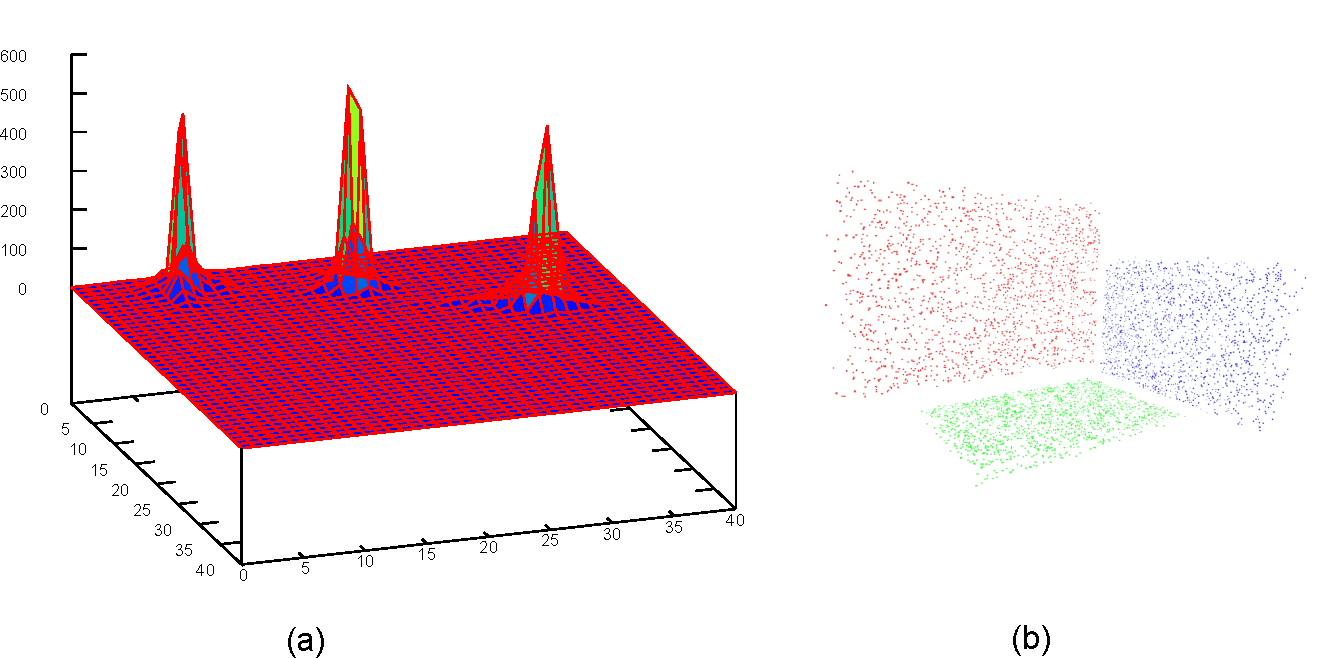
\includegraphics[width=\textwidth]{figures/ac-pole}
\caption{Ukázka akumulátorového pole (a), které representuje mračno bodů se třemi kolmými rovinami (b). Svislá osa grafu reprezentuje počet bodů, vodorovné osy parametry bodů (tedy souřadnice v poli).}
\label{fig:acc-pole}
\end{center}
\end{figure}

Pokud máme všechny body uloženy v akumulátorovém poli, vyhledáme buňku s největším počtem bodů (tedy nejvyšší vrchol). Velikost buňky v akumulátorovém poli je určena na základě velikosti šumu ve vstupním mračnu. Tyto body z nejvyššího vrcholu proložíme rovinou pomocí metody nejmenších čtverců. Poté ohodnotíme kvalitu roviny výpočtem efektivní hodnoty (anglicky root mean square, dále jen RMS) vzdáleností všech bodů od proložené roviny. Pokud máme množinu $n$ bodů $\left\{x_1, x_2, \ldots , x_n\right\}$ a jejich vzdáleností od proložené roviny $\left\{d_1, d_2, \ldots , d_n\right\}$, vypočítáme RMS podle vztahu \ref{eq:rms}:

\begin{equation} 
\label{eq:rms}
RMS = \sqrt{
\frac{1}{n}\left({d_1}^2 + {d_2}^2 + \ldots + {d_n}^2\right)
}
\end{equation}

Přijatelná hodnota je závislá na velikosti šumu v datech, obecně lze říct, že kvalita roviny je dostatečná, pokud je vypočtené RMS menší, než velikost šumu v datech. Pokud je RMS větší, pravděpodobně jsme detekovali výše popsaný problém, kdy více rovin splynulo v akumulátorovém poli do jednoho vrcholu. Řešení tohoto problému bude popsáno ke konci této sekce.

Pokud je tedy vypočtené RMS v přijatelných mezích, vytvoříme počáteční klastr, do kterého dáme všechny body dané buňky. Klastrování pokračuje body, které do této buňky nepatří, ale jsou v jejím okolí. Tento krok je nezbytný, protože data obvykle nebývají tak přesná, aby se všechny body z roviny trefily přesně na jedno místo v akumulátorovém poli, zejména jde o body v okolí hran a nerovností na povrchu. Tento postup probíhá iterativně a funguje tak, že v první iteraci je identifikováno 8 buněk v sousedství buňky s největším počtem bodů (viz Obr. \ref{fig:acc-pole-clus}). 

\begin{figure}[ht]
\begin{center}
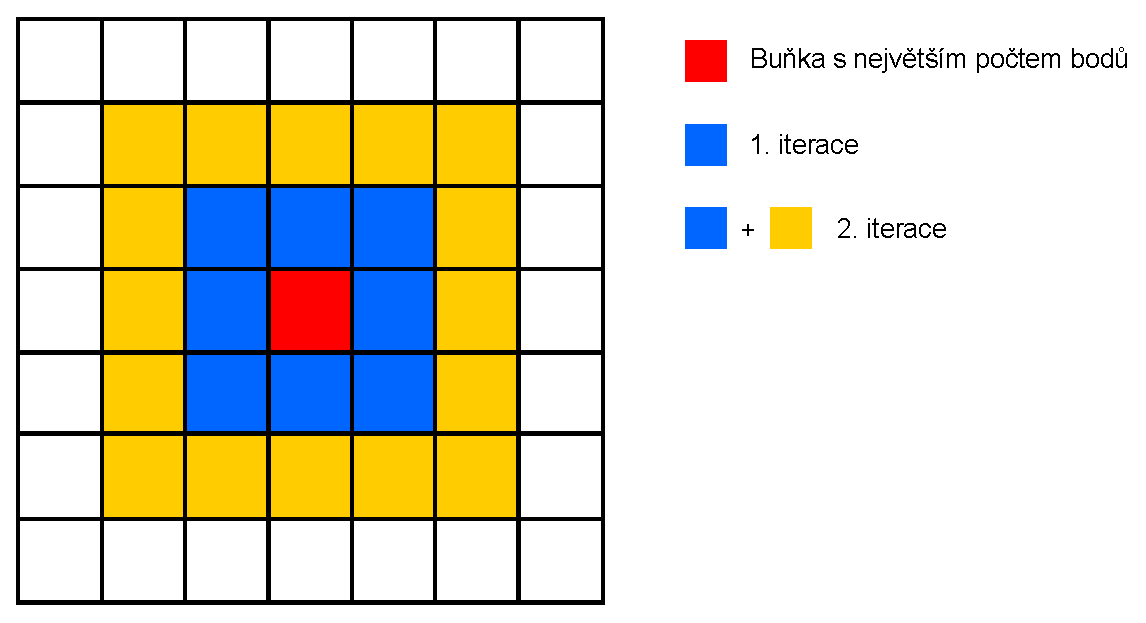
\includegraphics[width=12cm]{figures/acc-pole-clustering}
\caption{Prohledávání políček v akumulátorovém poli v průběhu jednotlivých iterací.}
\label{fig:acc-pole-clus}
\end{center}
\end{figure}

\noindent
Body z těchto osmi buněk přidáme do segmentu pouze, pokud splní dvě podmínky. První podmínkou je, že bod musí být prostorově blízko k bodům z původního klastru (např. 2x průměrná vzdálenost mezi body v původním klastru). Poté je spočítána vzdálenost bodů od roviny, která je definována body z původního klastru. Pouze body, které jsou k rovině blíže, než je předem daný práh, mohou být přidány do klastru. Tento práh je opět určen v závislosti na velikosti šumu v datech.  Body, které nesplnily jednou z těchto dvou podmínek zůstanou na své pozici v akumulátorovém poli a jsou znovu posouzeny v dalších iteracích. Po ukončení každé iterace se přepočítají parametry klastru - tedy opět se body proloží rovina, ale jsou zahrnuty i nově přidané body. Poté proces pokračuje druhou iterací. V té jsou procházeny body z 24 sousedních buněk (viz Obr. \ref{fig:acc-pole-clus}). Proces je navržen tak, aby v této iteraci byly opět procházeny i ty body, které neprošly podmínkami v předchozích iteracích. Protože se na konci každé iterace přepočítávají parametry, mohou být tyto body v dalších iteracích do klastru zahrnuty. Takto iterativně proces pokračuje až do té doby, než do klastru nemohou být přidány žádné nové body. V tu chvíli je klastr zaznamenán a všechny jeho body jsou odebrány z akumulátorového pole.

Nyní proces pokračuje k druhému nejvyššímu vrcholu v akumulátorovém poli, který je nalezen stejným způsobem, jako byl ten nejvyšší v předchozí iteraci. Poté se opakují stejné kroky, jako v předchozím případě. Celý tento proces přesouvání se od nejvyššího vrcholu k druhému nejvyššímu pokračuje až do té doby, dokud je velikost nejvyššího vrcholu menší, než předdefinovaná hranice.

Poslední součástí algoritmu je řešení situace, kdy více rovin sdílí stejný vrchol v akumulátorovém poli. Tuto situaci jsme již detekovali pomocí výpočtu RMS. Pokud je hodnota vypočteného RMS příliš vysoká, s velkou pravděpodobností jsou ve vrcholu body z více různých rovin. V takovém případě jsou definovány dva nové referenční body. Pozice nových referenčních bodů je definovaná podle vztahu \ref{eq:new-origins}:

\begin{center}
\begin{equation} 
\label{eq:new-origins}
$$
$\left( \begin{array}{ccc}
X_n \\
Y_n \\
Z_n
\end{array}\right)$ = 
$\left( \begin{array}{ccc}
X_o \\
Y_o \\
Z_o
\end{array}\right)$ 
+ 
$\left( \begin{array}{ccc}
range \times rand \\
range \times rand \\
range \times rand
\end{array}\right)$
$$
\end{equation}
\end{center}

\noindent
kde ($X_n$, $Y_n$, $Z_n$) jsou souřadnice nového bodu, ($X_o$, $Y_o$, $Z_o$) jsou souřadnice původního bodu, $range$ je hodnota určující jak nejdál může být nový bod posunut (např. 5m) a $rand$ je náhodná hodnota z intervalu (0,1).

Poté je definováno nové akumulátorové pole pouze pro tyto body (způsobující problém) a na základně nově definovaných referenčních bodů jsou přepočteny parametry bodů. Poté jsou vyhledány nově vytvořené vrcholy a ty jsou klastrovány stejným způsobem, jako v běžném případě. Tento proces se opakuje do té doby, než jsou nalezeny dostatečně kvalitní roviny. V případě, že do určitého počtu iterací (např. 10) není nalezena žádná přijatelná rovina, vezme se druhá nejvyšší buňka ze zpracovávaného vrcholu v původním poli, proloží se rovinou a ohodnotí se její kvalita výpočtem RMS. Poté proces pokračuje standardně jednotlivými kroky, které již byly popsané. Tento proces by měl v praxi nastat jen výjimečně, obvykle situace splynutí dvou vrcholů vůbec nenastane a pokud ano, s velkou pravděpodobností bude vyřešena hned po změně pozic referenčních bodů.

Tímto jsme popsali celý algoritmus. Jak by mělo být patrné, algoritmus bere v úvahu vztahy bodů v prostoru parametrů a zároveň jejich vzdálenost a umístění v prostoru. Navíc je tento algoritmus poměrně robustní, protože při klastrování mají prioritu body, které mají podobnější parametry a zároveň jsou blízko v prostoru, před body, jejichž parametry jsou více odlišné.


\section{Proložení roviny množinou bodů}
\label{sub:lsq}
Důležitou součástí algoritmu je proložení roviny množinou bodů pomocí metody nejmenších čtverců, viz \cite{wiki:leastsq}. Předpoklad tedy je, že chceme nalézt rovinu, která je co nejblíže od všech 3D bodů z dané množiny. Mějme množinu velikosti $k$, která obsahuje body ($p_1, \ldots, p_k$). Rovina je definována bodem $c$, který leží v rovině, a normálový vektorem $n$, který je na rovinu kolmý. Pro libovolný bod $x$ ležící v rovině platí vztah $n(x - c)^T = 0$. Pokud vezmeme bod $y$, který v rovině neleží, potom platí $n(y - c)^T \neq 0$. Je tedy vhodné definovat odchylku podle vztahu \ref{eq:odchylka}:

\begin{equation}
\label{eq:odchylka}
(n (p_i - c)^T)^2
\end{equation}

Proložená rovina má být co nejblíže ke všem bodům. Jinými slovy hledáme takové $n$, které minimalizuje celkovou odchylku všech bodů. Rovinu tedy můžeme získat vyřešením následujícího vztahu:

\begin{equation}
\label{eq:ls-min}
\min_{c,\|n\|=1} \sum\limits_{i=1}^k (n (p_i - c)^T)^2
\end{equation}

Řešení tohoto vztahu pro $c$ je:

\begin{equation}
c = \frac{1}{k} \sum\limits_{i=1}^k p_i
\end{equation}

Bod $c$ je tedy aritmetickým průměrem všech prokládaných bodů (pro tento bod se používá označení centroid). Pokud si definujeme matici $M$, která má v $i$-tém řádku hodnoty $p_i - c$ (jde tedy o matici $k \times 3$), můžeme vztah  \ref{eq:ls-min} přepsat do této formy:

\begin{equation}
\min_{\|n\|=1} \|M n\|^2
\end{equation}

Řešením tohoto problému je SVD dekompozice matice $M$, $M = USV^T$, kdy vektor $n$ je určen pravým singulárním vektorem matice $M$, který odpovídá nejmenší singulární hodnotě. Konkrétně jde o poslední sloupec matice $V^T$.

Pokud tedy máme vypočtený bod $c$ a získali jsme normálový vektor $n$, můžeme snadno vyjádřit rovinou např. obecnou rovnicí:

\begin{equation}
ax + by + cz + d = 0
\end{equation}

\noindent
ve které parametry $a, b, c$ jsou složky normálového vektoru $n$ a $d$ spočteme jednoduše dosazením bodu $c$:

\begin{equation}
\label{eq:d}
d = -(n_1c_1 + n_2c_2 + n_3c_3)
\end{equation}

Toto řešení předpokládá, že všechny body mají stejnou váhu. Pokud máme pro body různé váhy, do výpočtu je zahrneme poměrně jednoduše. Pokud má bod $p_i$ váhu $w_i$, musíme vztah \ref{eq:ls-min} upravit tímto způsobem:

\begin{equation}
\min_{w_i,c,\|n\|=1} \sum\limits_{i=1}^k w_i \times (n (p_i - c)^T)^2
\end{equation}

Stejně musíme upravit definici matice $M$, která bude v každém řádku obsahovat hodnoty $w_i \times (p_i - c)$. Ostatní postup zůstává stejný.

%*****************************************************************************
\chapter{Implementace}
\label{chap:implementace}

Tato kapitola se zabývá popisem implementace algoritmu. Algoritmus je implementován v jazyce Java v rámci dodaného softwaru ArchiRec3D \cite{AR3D}. Kompletní zdrojový kód je k dispozici na přiloženém CD, viz kapitola~\ref{chap:CD}.


Implementaci algoritmu můžeme rozdělit na dvě hlavní části. První částí je výpočet parametrů pro všechny body a uložení bodů do akumulátorového pole. Druhou částí bude poté klastrování bodů v akumulátorovém poli. Tyto dvě části budou reprezentovány jako samostatné metody. První metoda bude mít na vstupu zpracovávané mračno bodů a jejím výstupem bude akumulátorové pole naplněné všemi body ze vstupního mračna. Druhá metoda bude mít toto akumulátorové pole na vstupu a výstupem budou body rozdělené do jednotlivých segmentů. Takovéto rozdělení má hlavní výhodu v tom, že obě části budou na sobě nezávislé. Bude tedy možné jednou uložit body do akumulátorového pole a poté provést klastrování několikrát s různými parametry bez nutnosti znovu provádět první část.

\section{Uložení bodů do akumulátorového pole}

Tato část algoritmu bude procházet všechny body, na základě jejich okolí bude vypočítávat parametry, podle kterých budou body uloženy do akumulátorového pole. Vstupem bude tedy mračno bodů a výstupem akumulátorové pole. Prvním problémem bude tedy to, jak v paměti správě reprezentovat obě tyto struktury. To se samozřejmě musí odvíjet od operací, které budeme s daty provádět. Protože algoritmus implementuji v rámci dodaného nástroje, mám k dispozici několik základních datových struktur jako např \verb|vicitis.inner.Point3D| pro reprezentaci 3D bodu, \verb|vicitis.inner.Plane3D| pro reprezentaci roviny apod., tyto datové struktury samozřejmě využiji. Navíc je zde také implementováno mnoho vhodných metod využívajících tyto třídy, takže je logické použít již funkční řešení a nevymýšlet vlastní, které by bylo navíc duplicitní.

Základním požadavkem na datovou strukturu reprezentující mračno bodů je možnost vyhledávat sousední body v 3D prostoru. Protože tuto operaci je nutné provádět pro každý bod, je důležité, aby byla co nejrychlejší. Naopak vytváření struktury se bude provádět pouze jednou a už do ní nebudeme za běhu přidávat ani odebírat body, takže na tyto operace nemusí být kladeny velké nároky. Pro tyto účely se nejčastěji využívají stromy, které umožňují rekurzivní dělení n-dimenzionálního prostoru na menší podprostory. Jedním z takovýchto algoritmů je octree, který rekurzivně dělí prostor na 8 podprostorů. Podobný algoritmus je kd-strom \cite{wiki:kdtree}, kde uzly jsou k-dimenzionální body. Tento typ stromu dělí prostor na podprostory podél jednotlivých dimenzí. Pokud srovnáme tyto dva algoritmy, tak octree se rychleji staví a zároveň umí jednoduše přidávat nové body do již postaveného stromu. Oproti tomu do kd-stromu se body za běhu přidávají mnohem složitěji, ale algoritmus je efektivnější pro vyhledávání bodů a nejbližších sousedů. Protože jsem určil rychlé vyhledávání nejbližších sousedů jako nejdůležitější kritérium, vybral jsem nakonec pro reprezentaci mračna bodů kd-strom. Vyhledání nejbližšího souseda v kd-stromu (o $n$ prvcích a $k$ dimenzích) má v nejlepším případě asymptotickou složitost $O(log~n)$ a v nejhorším případě $O(k \times n^{1-\frac{1}{k}})$, ve většině případů má však složitost blíže k nejlepšímu případu. Podrobný popis kd-stromu je k dispozici v \cite{wiki:kdtree}. Samozřejmě implementace kd-stromu je poměrně složitá, obzvláště, pokud má být co nejefektivnější. Proto jsem se rozhodl pro použití knihovny. Po vyzkoušení několika různých knihoven byla jednoznačně nejrychlejší implementace \cite{kdtree}, kterou jsem použil.

Pro akumulátorové pole potřebujeme nějaké dvourozměrné pole, které nám bude udržovat body  s danými parametry na jednotlivých pozicích v poli. Bylo by možné použít obyčejné \verb|int[][]| pole, které by pouze ukládalo počet bodů na jednotlivých políčkách. Takové řešení by na první pohled mohlo pro vyhledávání vrcholů při klastrování dostatečné, nicméně by bylo výpočetně náročné zpětně zjistit, které body na dané pozici jsou. Proto bude jednodušší, když budou body uložené přímo v akumulátorovém poli. Proto jsem zvolil 2D pole seznamů \verb|ArrayList<Point3D>[][]|, které bude udržovat body na jednotlivých políčkách pole. Takto budu při vyhledávání vrcholů v poli jednoduše vědět, kolik bodů se na daném políčku nachází, ale zároveň půjde tyto body ihned zpracovávat bez dalšího vyhledávání. 

Velmi důležité jsou také rozměry akumulátorového pole. Podle teorie je velikost políčka v akumulátorovém poli určena na základě velikosti šumu ve vstupním mračnu. Bohužel testovací data, která mám k dispozici, nemají šum definovaný. Proto je nutné vymyslet vlastní strategii pro určení velikosti akumulátorového pole. Pokud je akumulátorové pole příliš malé, jednotlivé vrcholy mohou splynout, nepůjde je v poli detekovat a algoritmus prakticky nebude funkční. Pokud naopak bude akumulátorové pole příliš velké, vrcholy v poli nebudou výrazné a výsledek bude stejný jako v předchozím případě - algoritmus nebude fungovat tak, jak by se od něj čekalo. Původně jsem vycházel z úvahy, že velikost políčka v akumulátorovém poli bude např. jedna tisícina z velikosti mračna bodů. V takovém případě je ale velikost pole pro všechny vstupní data stejná (např. $1000~\times~1000$). To ale není vhodné řešení, protože vstupní data mohou obsahovat řádově tisíce až miliony bodů a nezdá se logické, aby pro oba případy bylo akumulátorové pole stejně velké (a v praxi se to také ukázalo jako nefunkční řešení). Z toho jsem tedy usoudil, že velikost akumulátorového pole bude výrazně závislá na počtu vstupních bodů. Proto se zdá rozumné odvodit velikost pole právě od této hodnoty. Nejprve jsem zkusil určit velikost pole jako tisícinu z počtu bodů. To se také neukázalo jako vhodné řešení, protože pro malá mračna bylo pole příliš malé a pro velká mračna naopak příliš velké (pro 1,5 milionu bodů by bylo potřeba alokovat pole o rozměrech $15000~\times~15000$, což by bylo paměťově extrémně náročné). Lineární závislost mezi počtem bodů a velikostí akumulátorového pole tedy není správné řešení. Došel jsem tedy k úvaze, že by mohlo být vhodné zvolit stejný počet políček v akumulátorovém poli, jako je počet bodů. To nám zajistí, že pole nikdy nebude příliš malé, protože se předpokládá, že body ležící ve stejné rovině budou jen v několika sousedních políčkách. Proto by mělo v poli zbýt dostatek volných políček, aby jednotlivé vrcholy nesplynuly dohromady. Po vyzkoušení na reálných datech jsem zjistil, že velikost pole není ani příliš velká a vrcholy jsou dostatečně výrazné. Jako rozměr akumulátorového pole jsem tedy určil odmocninu z počtu bodů (to odpovídá stavu, že počet políček v poli se rovná počtu bodů). V takovém případě je pro mračno s 10 tisíci body alokováno pole velikosti $100~\times~100$, pro 1,5 milionu bodů je to pole o rozměrech $1225~\times~1225$. Samozřejmě ani toto není optimální řešení. Velikost pole by měla být nejlépe odvozena od konkrétního zpracovávaného mračna a jeho vlastností jako očekávaný počet rovin, hustota bodů, počet bodů mimo roviny apod. Nicméně takový algoritmus by nebyl vůbec jednoduchý a pravděpodobně by vyžadoval nějaké vstupní parametry zadané uživatelem. To je ale nevhodné, za prvé se očekává, že algoritmus bude co nejvíce automatický, za druhé by běžný uživatel bez hlubších znalostí nebyl schopen takové parametry zadat. Proto jsem nakonec zvolil uvedené řešení.

Nyní máme připravené potřené datové struktury, můžeme tedy začít se samotným algoritmem. Nejprve si tedy vytvoříme novou instanci kd-stromu, konkrétně instanci třídy \verb|SqrEuclid|, což je kd-strom, který využívá klasickou euklidovskou vzdálenost mezi body. Poté kd-strom  v cyklu naplníme body a zároveň získáme jednoduchým porovnáním  největší a nejmenší hodnoty souřadnic v celém mračnu bodů. Tyto souřadnice využijeme k výpočtu pozic referenčních bodů podle vztahu \ref{eq:origins}.

Ještě před samotným výpočtem parametrů bodů musíme stanovit velikost koule, která definuje okolí (viz sekce \ref{sub:def-okoli}). V popisovaném článku je tato velikost udávána euklidovskou vzdáleností (např. 3m). Já ale v testovacích datech žádné měřítko nemám, navíc mně dostupná data jsou poměrně odlišná od dat, které používali pro testování v článku. Proto je tato definice nevhodná a je potřeba ji nějak obejít. Protože mohou mít různá data výrazně jinou hustotu bodů, přijde mi rozumné velikost koule vypočítat z daného konstantního počtu bodů. Bohužel určit tento počet naprosto obecně pro libovolný typ dat je téměř nemožné. Proto jsem se rozhodl nechat tuto hodnotu jako volný parametr, který bude zadán uživatelem. To má i další důvod, tato hodnota velmi zásadně ovlivňuje dobu běhu algoritmu. Vyhledávání okolí v kd-stromu je drahá operace a pokud se pro každý bod vyhledává okolí v řádu stovek bodů, algoritmus může běžet desítky minut, což jistě není vždy optimální. Zároveň ale do určité míry platí, že čím větší okolí bodu se bere v úvahu, tím přesnější jsou vypočtené parametry bodu. Tím, že necháváme tento parametr na uživateli, mu dáváme možnost vybrat si mezi rychlostí nebo kvalitou. Pokud tedy uživatel zadá malé hodnoty tohoto parametru, např. 10 - 40, tak je algoritmus poměrně rychlý, ale může vracet horší výsledky. Pokud zadá větší hodnoty, např. 80 - 200, tak může být doba běhu algoritmu výrazně pomalejší, zato s kvalitnějšími výsledky. Obecně bych doporučil volit hodnoty z intervalu 20 - 200 s tím, že vhodný kompromis mezi kvalitou a rychlostí je obvykle 40 - 80. Konkrétní dopad těchto hodnot na dobu běhu a kvalitu segmentace bude popsán v kapitole \ref{chap:test}. Je důležité zmínit, že tato hodnota se musí odvíjet zejména od vstupních dat, nikoliv pouze od toho, zda chceme kvalitu nebo výkon. Pokud máme data hodně přesná (tedy body v rovině mají od této roviny jenom minimální odchylku), můžeme volit menší hodnoty pro velikost okolí a výsledek bude stále kvalitní. Pokud máme ale např. data reprezentující budovu s nerovným povrchem (např. s taškovou střechou), který chceme rozpoznat jako segment, musíme volit okolí větší. Na obrázku \ref{fig:strecha} je ukázka takové situace, kdy volba příliš malého okolí značně ovlivní výsledný výpočet.

\begin{figure}[ht]
\begin{center}
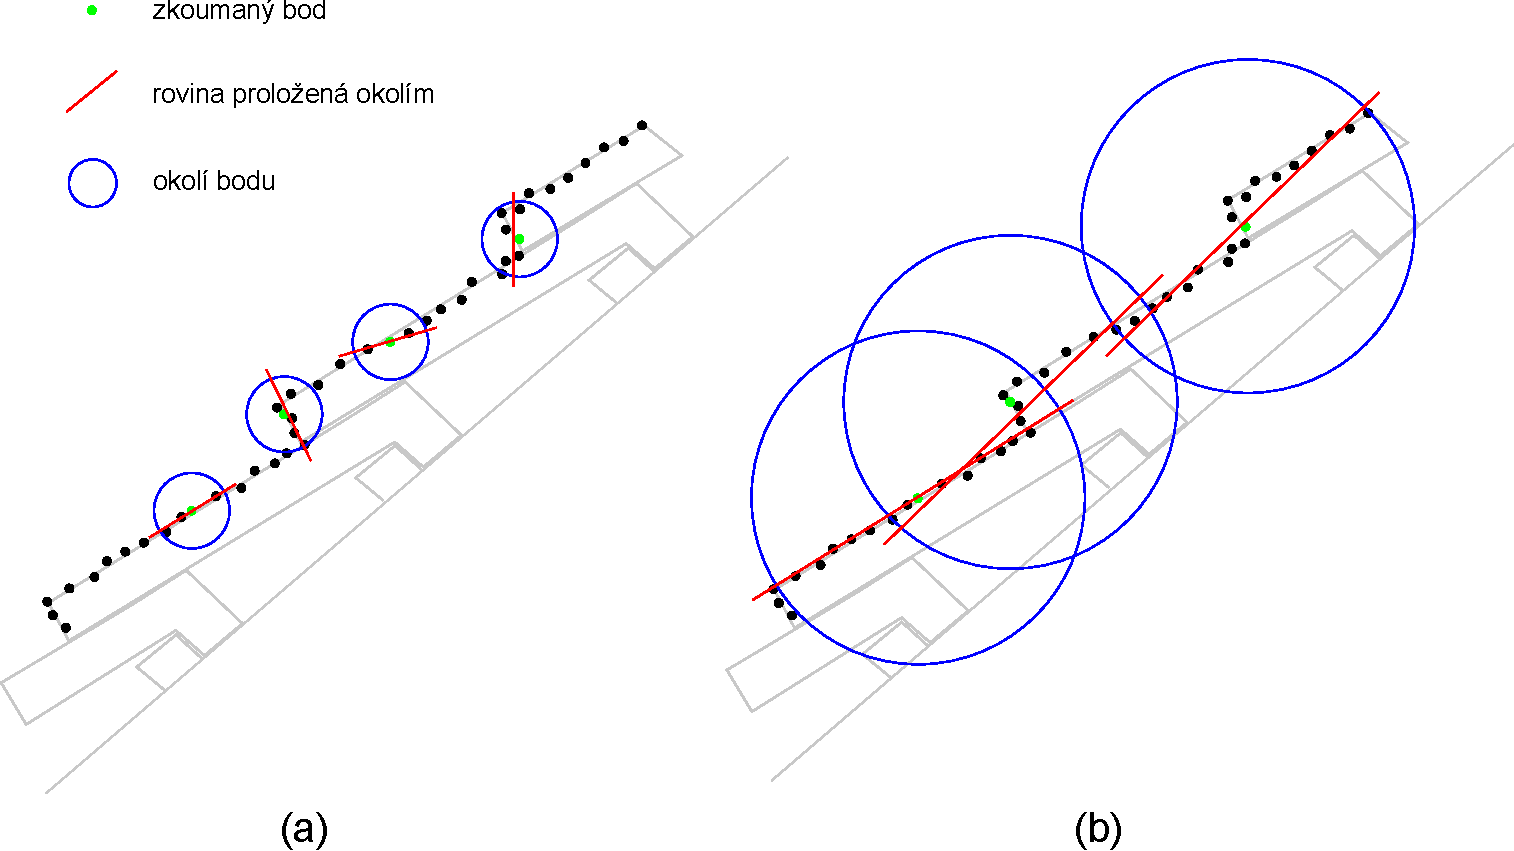
\includegraphics[width=\textwidth]{figures/strecha-all}
\caption{Ukázka vlivu velikosti okolí na vypočítávané parametry. Malé okolí může způsobit chybný výpočet (a), oproti tomu velké okolí je přesnější (b).}
\label{fig:strecha}
\end{center}
\end{figure}

Hodnota, kterou uživatel zadá, se ještě přímo nevyužije k definici okolí. Tato hodnota se využije pouze k vypočtení velikosti výsledné koule. Výpočet probíhá tak, že se náhodně vybere z mračna určitý počet bodů (např. setina ze všech bodů). Pro každý náhodně vybraný bod se vybere takový počet nejbližších sousedů, jaká je hodnota zadaného parametru. Poté se spočítá poloměr koule, které vybrané body tvoří (tedy vzdálenost střed - nejvzdálenější bod). Nakonec se spočítá aritmetický průměr všech vypočtených poloměrů. Tento aritmetický průměr je konečná velikost koule, která bude v algoritmu definovat okolí bodu. Pro všechny body bude mít tedy okolí stejnou velikost, ale bude pokaždé obsahovat různý počet bodů.

V tuto chvíli již máme všechny potřebné informace pro výpočet parametrů všech bodů. Máme načtené body v kd-stromu, máme definované oba referenční body, dále máme vypočtenou velikost koule pro okolí bodu a máme připravené akumulátorové pole, do kterého budeme body ukládat. Vytvoříme tedy cyklus, pomocí kterého budeme procházet všechny body v mračnu.

Nyní potřebujeme pro každý bod získat jeho okolí, tedy všechny body, které leží v kouli se středem v daném bodu a poloměrem, který jsme vypočítali. Víme, kolik průměrně bodů by mělo v této kouli být. Pro první iterovaný bod tedy vezmeme tento počet nejbližších sousedů. Vyhledávání $n$ nejbližších sousedů je v kd-stromu definovaná operace, takže je to velmi jednoduché. Dále si spočítáme vzdálenost zkoumaného bodu a nejvzdálenějšího bodu z vybraných sousedů (kd-strom vrací body seřazené podle vzdálenosti od původního bodu, takže nejvzdálenější bod je ten poslední v seznamu). Pokud je tato vzdálenost větší, než je velikost koule definující okolí, tak pomocí binárního prohledávání projdeme seznam sousedů a nalezneme nejvzdálenější bod, který ještě leží uvnitř koule. Všechny body, které jsou dál, zahodíme. Pokud nastane situace, kdy ještě nemáme dostatek bodů, vynásobíme aktuální počet vybraných sousedů 1,5$\times$ a tento nový počet opět vybereme z kd-stromu a testujeme. Takto pokračujeme do té doby, než máme dostatek bodů. Je potřeba zmínit, že tento iterativní proces by měl nastat co nejméně, protože vyhledávání nejbližších sousedů v kd-stromu je pomalá operace. Celý výše popsaný proces získávání bodů pro okolí je přehledně znázorněn na diagramu \ref{fig:diag-okoli}.

\begin{figure}[ht]
\begin{center}
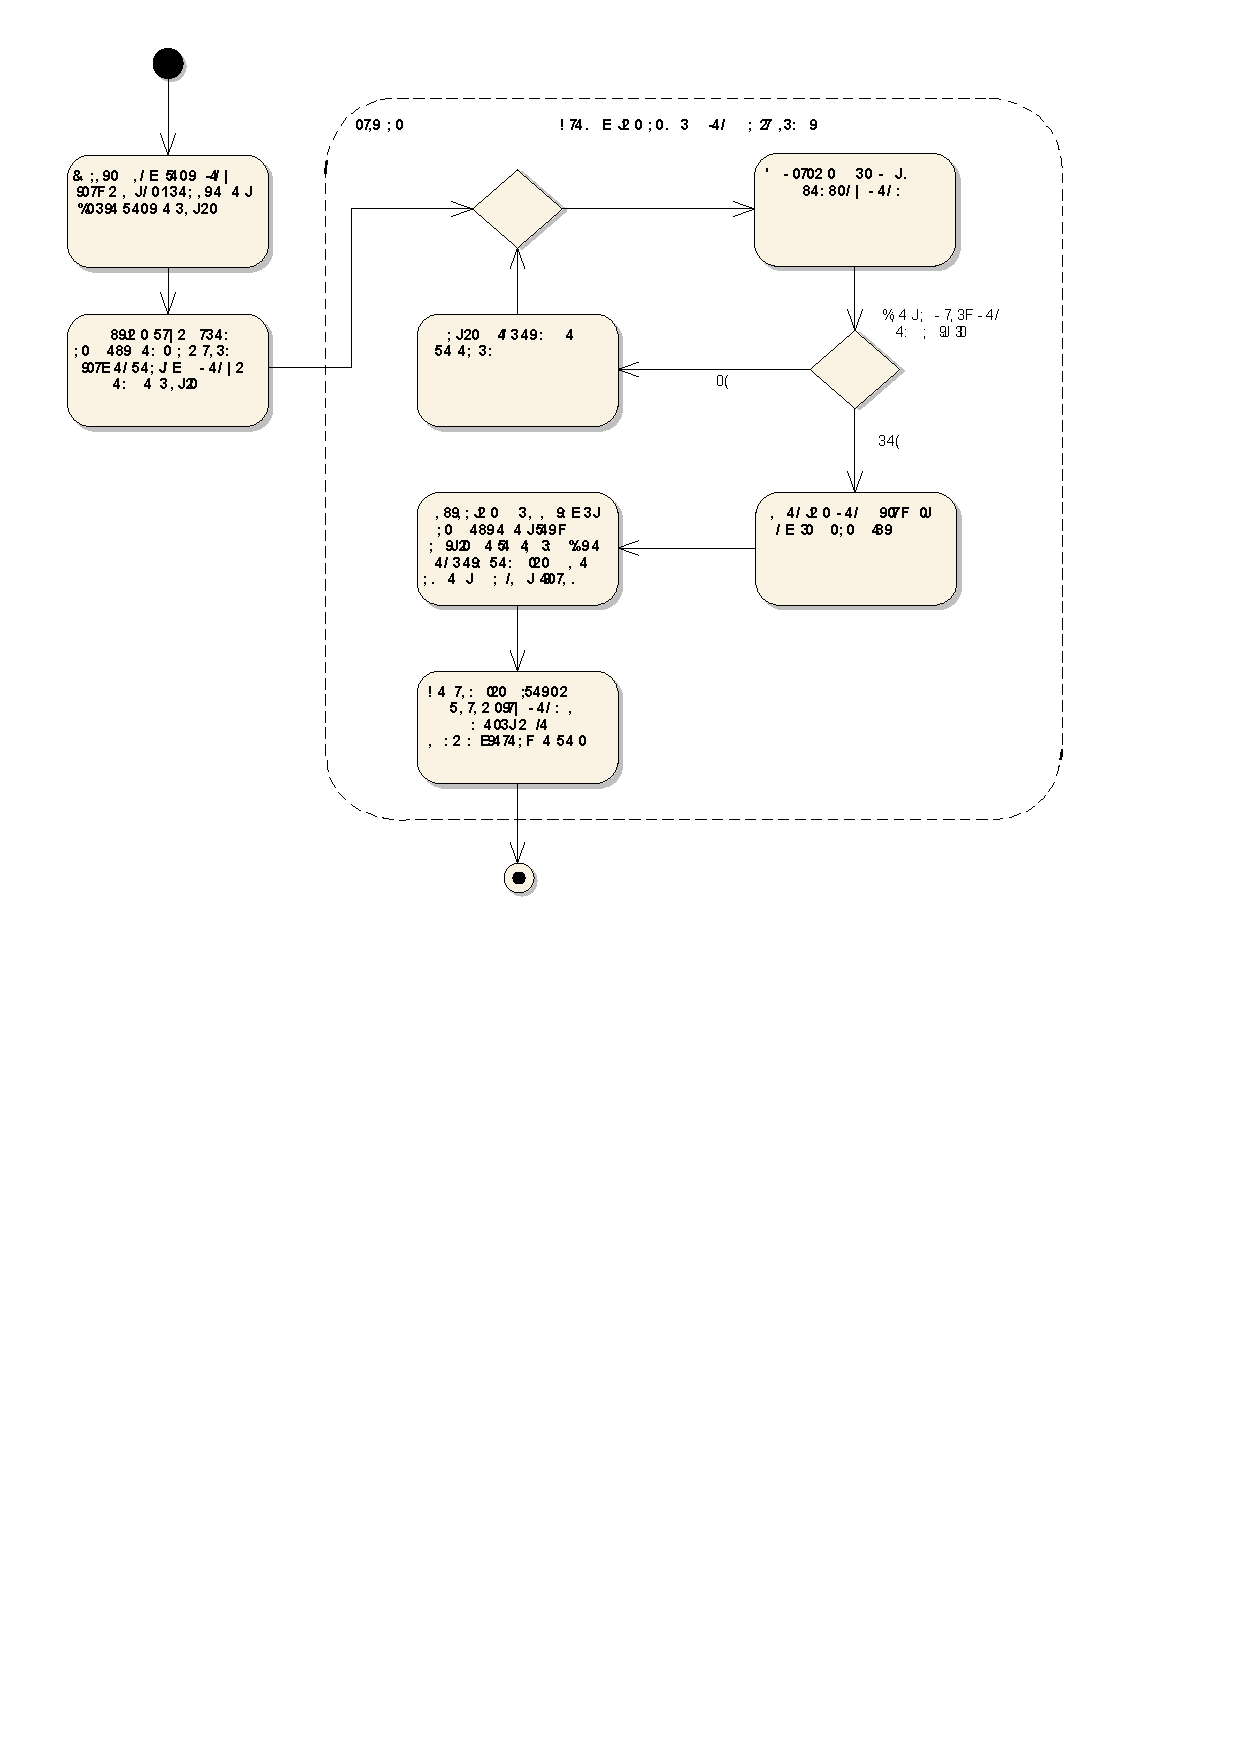
\includegraphics[width=\textwidth]{figures/okoli-diagram-algoritmus}
\caption{Diagram znázorňující získání potřebných nejbližších sousedů bodu.}
\label{fig:diag-okoli}
\end{center}
\end{figure}

Protože blízké body v mračnu bodů budou mít pravděpodobně velmi podobné okolí, využijeme výslednou velikost okolí jako výchozí hodnotu pro bod v další iteraci\footnote{Očekáváme tedy, že body na vstupu jsou nějakým způsobem seřazené, a že v naprosté většině případů jsou dva po sobě jdoucí body velmi blízko v prostoru.}. Tady nastává otázka, jestli použít přesně tu samou hodnotu nebo jí o trochu zvýšit. Vyhledávání bodů v kd-stromu je pomalá operace a nechceme, aby bylo v další iteraci zbytečně provedeno dvakrát, protože chybělo několik málo bodů. Zároveň je ale nutné vzít v úvahu, že čím více bodů v kd-stromu vyhledáváme, tím pomalejší toto vyhledávání je. Je tedy otázka, jaký je optimální poměr navýšení počtu bodů do další iterace. Proto jsem se rozhodl určit tento parametr experimentálně. Porovnal jsem 3 různá vstupní mračna o rozdílných velikostech a volil jsem velikost okolí 50 a 200 bodů. V tabulce \ref{table:okoli-param} je zaznamenán celkový čas, který vybírání sousedních bodů zabralo a také je zde uvedeno procento bodů, pro které bylo nutné vyhledávat v kd-stromu vícekrát\footnote{Tato informace je pouze pro zajímavost, relevantní pro porovnání je pouze celkový čas.}. V naprosté většině případů byly výsledky nejlepší při hodnotě parametru 1,10. Pro další bod při iterování bude tedy použit 1,1$\times$ násobek aktuální velikosti okolí.


\begin{table}[ht]
\resizebox{\textwidth}{!} {
\begin{tabular}{|l|r|r|r|r|r|r|r|r|r|r|r|r|}
\hline
\textit{} & \multicolumn{ 4}{c|}{\textit{Data 1: 291232 bodů}} & \multicolumn{ 4}{c|}{\textit{Data2: 81294 bodů}} & \multicolumn{ 4}{c|}{\textit{Data3: 1299900 bodů}} \\ \hline
\textit{Okolí} & \multicolumn{ 2}{c|}{\textit{50 bodů}} & \multicolumn{ 2}{c|}{\textit{200 bodů}} & \multicolumn{ 2}{c|}{\textit{50 bodů}} & \multicolumn{ 2}{c|}{\textit{200 bodů}} & \multicolumn{ 2}{c|}{\textit{50 bodů}} & \multicolumn{ 2}{c|}{\textit{200 bodů}} \\ \hline
\textit{Param.} & \textit{Opak.} & \textit{Čas} & \textit{Opak.} & \textit{Čas} & \textit{Opak.} & \textit{Čas} & \textit{Opak.} & \textit{Čas} & \textit{Opak.} & \textit{Čas} & \textit{Opak.} & \textit{Čas} \\ \hline
1,00 & 50,83\% & 21,67 & 51,45\% & 79,67 & 49,59\% & 6,15 & 49,83\% & 22,54 & 50,51\% & 135,52 & 50,52\% & 659,17 \\ \hline
1,05 & 27,43\% & 17,04 & 16,84\% & 56,95 & 33,06\% & 5,35 & 24,92\% & 18,01 & 27,69\% & 114,88 & 15,84\% & 452,84 \\ \hline
\textbf{1,10} & \textbf{17,89\%} & \textbf{15,19} & \textbf{10,11\%} & \textbf{53,28} & \textbf{24,67\%} & \textbf{4,51} & \textbf{16,70\%} & \textbf{17,38} & \textbf{17,36\%} & \textbf{110,57} & \textbf{9,31\%} & \textbf{457,39} \\ \hline
1,15 & 12,88\% & 16,18 & 7,31\% & 57,25 & 18,64\% & 5,14 & 12,36\% & 19,69 & 12,60\% & 111,30 & 6,72\% & 488,15 \\ \hline
1,25 & 8,04\% & 16,49 & 4,93\% & 60,14 & 13,89\% & 4,55 & 8,70\% & 20,54 & 7,98\% & 120,90 & 4,38\% & 522,85 \\ \hline
1,50 & 4,26\% & 17,99 & 2,91\% & 70,07 & 7,72\% & 5,07 & 5,34\% & 21,17 & 3,79\% & 133,85 & 2,48\% & 604,66 \\ \hline
2,00 & 2,17\% & 23,90 & 1,62\% & 99,68 & \multicolumn{1}{l|}{} & \multicolumn{1}{l|}{} & \multicolumn{1}{l|}{} & \multicolumn{1}{l|}{} & \multicolumn{1}{l|}{} & \multicolumn{1}{l|}{} & \multicolumn{1}{l|}{} & \multicolumn{1}{l|}{} \\ \hline
2,50 & 1,51\% & 26,34 & 1,15\% & 121,76 & \multicolumn{1}{l|}{} & \multicolumn{1}{l|}{} & \multicolumn{1}{l|}{} & \multicolumn{1}{l|}{} & \multicolumn{1}{l|}{} & \multicolumn{1}{l|}{} & \multicolumn{1}{l|}{} & \multicolumn{1}{l|}{} \\ \hline
\end{tabular}
}
\caption{Tabulka znázorňující rozdílné časy vybírání okolí z kd-stromu v závislosti na definovaném parametru. Čas je uváděn v sekundách, sloupec \uv{Opak.} určuje, pro jaké procento bodů bylo nutné z kd-stromu vybírat okolí více než jednou. Prázdná políčka jsem již nevyplňoval, protože předešlé výsledky byly dostatečně průkazné a další měření by bylo zbytečné.} 
\label{table:okoli-param}
\end{table}

V tuto chvíli máme pro bod vybrány všechny sousední body, které leží uvnitř dané koule. Abychom získali konečné okolí bodu, musíme proložit body rovinou a poté provést převažování této roviny pomocí procesu popsaného v sekci \ref{sub:def-okoli}. Dalším krokem v algoritmu je tedy pomocí metody nejmenších čtverců proložit rovinu body uvnitř koule.

Teorie k proložení roviny množinou bodů pomocí metody nejmenších čtverců je popsána v sekci \ref{sub:lsq}. Implementace této metody přímo vychází z teorie. Prvním krokem je výpočet centroidu, což je bod ležící na výsledné rovině. Tento bod se spočte jednoduše jako aritmetický průměr souřadnic všech vstupních bodů. Poté se vytvoří matice, které má 3 sloupce a stejný počet řádků, jako je vstupních bodů. Na $i$-tém řádku je po souřadnicích zapsán rozdíl hodnot $bod_i - centroid$. Nad touto maticí je nutné provést SVD dekompozici. Poté stačí pouze vybrat z matice $V^T$ poslední sloupec a dopočítat koeficient $d$, viz vztah \ref{eq:d}. Tím získáme všechny 4 potřebné parametry a můžeme vrátit novou instanci roviny.

Ještě je nutné uvést, jak se provede SVD dekompozice. To je poměrně složitý a výpočetně náročný algoritmus, takže má smysl využít nějakou kvalitní matematickou knihovnu. Těch je ale velký počet a mohou se výrazně lišit ve výkonu. Na webových stránkách \cite{svdbench} je dostupné srovnání výkonu několika nejběžnějších knihoven pro matematické výpočty. Na obrázku \ref{fig:svd-bench} je graf, který znázorňuje výkon jednotlivých knihoven při výpočtu SVD.

\begin{figure}[ht]
\begin{center}
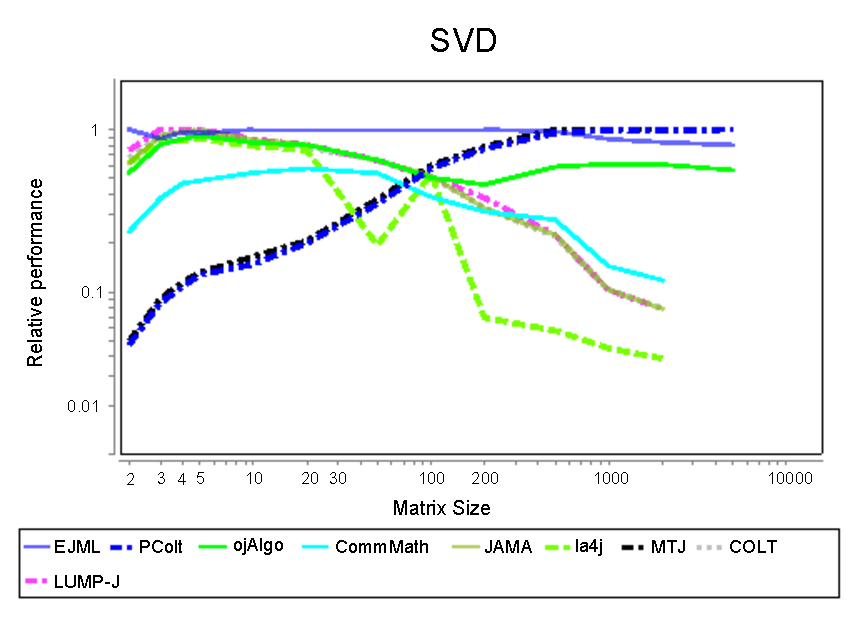
\includegraphics[width=10cm]{figures/svd}
\caption{Graf znázorňující relativní výkon (1 = nejvyšší výkon) různých knihoven při SVD dekompozici. Obrázek je převzat z \cite{svdbench}.}
\label{fig:svd-bench}
\end{center}
\end{figure}

Nejlépe z testu vychází knihovna EJML \cite{svdlib}. Nicméně je nutné poznamenat, že tato knihovna je od stejného autora, jako je daný test. Proto jsem se rozhodl provést vlastní test na reálných datech. Nedělal jsem žádný speciální test, pouze jsem měnil knihovny pro výpočet SVD v rámci již hotového algoritmu. Použil jsem mračno 389002 bodů, nastavil velikost okolí 100 bodů\footnote{To odpovídá průměrně 100 bodům v okolí, tedy i matici 3x100 při výpočtu SVD.} a měřil jsem čas, který výpočet SVD zabere. Měření je uvedeno v tabulce \ref{table:svdlib}.

\begin{table}[ht]
\resizebox{\textwidth}{!} {
\begin{tabular}{|r|r|r|r|r|r|r|r|}
\hline
\textbf{Měření} & \textbf{EJML*} & \textbf{EJML} & \textbf{Jama*} & \textbf{UJMP} & \textbf{CommMath} & \textbf{Colt} & \textbf{jBlas} \\ \hline
\textbf{1} & 88,958 & 136,998 & 152,786 & 157,150 & 185,178 & 206,535 & $>$300,000 \\ \hline
\textbf{2} & 88,860 & 135,831 & 151,418 & 156,057 & 182,576 & 201,198 & - \\ \hline
\textbf{Ø} & 88,909 & 136,415 & 152,102 & 156,604 & 183,877 & 203,867 & $>$300,000 \\ \hline
\end{tabular}
}
\caption{Tabulka znázorňující časy výpočtu SVD různých knihoven. Časy jsou uvedeny v sekundách. Knihovny označené * jsou nastavené tak, aby při SVD počítaly pouze matici $V^T$.} 
\label{table:svdlib}
\end{table}

Jak je z tabulky patrné, nejrychlejší je knihovna EJML, stejně jako ve výše uvedeném testování. Rozdíl byl natolik výrazný, že jsem provedl pouze dvě měření, přišlo mi zbytečné měření opakovat na jiných datech. Navíc EJML umožňuje při SVD vypočítávat pouze matici $V^T$, která je pro proložení roviny potřebná, což výrazně zvyšuje celkový výkon. Z těchto důvodů jsem se rozhodl pro výpočty SVD využít EJML.

Dříve v této kapitole jsem odůvodňoval, proč je průměrná velikost okolí zadávána u\-ži\-va\-te\-lem. Jedním z argumentů bylo, že uživatel si částečně může zvolit, jestli chce segmentaci provést rychle nebo spíše pomaleji a kvalitněji. Je potřeba zmínit, že rychlost algoritmu není daná pouze vybíráním okolí z kd-stromu. Další velkou složkou z celkového času je právě výpočet SVD při prokládání roviny. Ve skutečnosti prokládání bodů rovinou zabere větší část z celkového času běhu algoritmu, než vybírání bodů z kd-stromu. Nicméně obě tyto hodnoty jsou řádově stejné a dohromady tvoří velkou část z celkové doby běhu. Stejně jako u kd-stromu je i prokládání bodů rovinou je výrazně závislé na počtu vstupních bodů. Mělo by tedy být jasné, že velikost okolí naprosto zásadně ovlivňuje dobu běhu celého algoritmu, uživatel může tedy vhodnou volbou okolí výrazně přizpůsobit celkový čas algoritmu svým potřebám.

Zpět k implementaci algoritmu: jsme ve fázi, kdy máme vybrané okolí bodu a tímto okolím jsme proložili rovinu. Je nutné zmínit, že při prokládání roviny může nastat výjimka, kdy bod nemá žádný bod ve svém okolí nebo má jenom jeden. V takovém případě není proložení roviny z principu možné. Pro takovýto bod tedy nemůžeme vypočítat parametry a je nutné ho zahodit. Nicméně takových bodů by mělo být naprosté minimum a vzhledem k tomu, že bod nemá okolí, tak velmi pravděpodobně neleží na žádné rovině a jde spíš o nějakou chybu ve vstupních datech, takže jeho zahození nepředstavuje problém. 

Pokud se rovinu podaří proložit, pokračujeme úpravou této roviny pomocí převažování. Nejprve pro každý bod spočítáme váhu, což je inverze ke vzdálenosti bodu od roviny. Po vypočítání všech vah proložíme znovu rovinu všemi body, nicméně tentokrát využijeme váhy a váženou metodu nejmenších čtverců. Implementace vážené varianty metody nejmenších čtverců je téměř stejná jako běžné varianty, jenom se uvažují váhy při výpočtu centroidu a při konstrukci matice, nad kterou se poté provádí SVD. Po proložení roviny se rozhoduje, zda se opět vypočítají váhy a rovina se znovu proloží nebo zda se cyklus ukončí. Ukončení cyklu nastává ve dvou případech, pokud jsme již v desáté iteraci nebo pokud se parametry nové roviny výrazně neliší od poslední iterace. To zjistíme tak, že si udržujeme normálový vektor roviny z předchozí iterace a zjistíme jeho odchylku od normálového vektoru roviny ze současné iterace. Pokud je odchylka menší než cca. $2^\circ$, tak cyklus ukončíme.

Ačkoliv tento proces převažování vypadá na první pohled jednoduše, je zde malý problém s výpočtem vah, které se v rámci iterací mění pomalu a provádí se zbytečně velký počet iterací. Jako řešení se nabízí použít inverzi k druhé mocnině vzdálenosti bodu od roviny. Toto řešení funguje poměrně dobře a výrazně snižuje potřebný počet iterací a tím i celkový čas běhu algoritmu. Nicméně i toto řešení má jeden problém, váhy bodů blízko rovině mohou narůstat do výrazně velkých čísel, což může ovlivnit výsledek. Problém nastává také v okamžiku, kdy bod leží přímo na dané rovině. V tu chvíli jeho váha odpovídá hodnotě $^1/_0$, což Java převede na hodnotu \verb|Double.INFINITY|. Pokud se takováto váha dostane do výpočtu SVD, tak sice nevznikne žádná výjimka a výpočet proběhne, nicméně výsledek výpočtu je vždy chybný. Tento problém jsme se snažil vyřešit tím, že jsem hodnotu nekonečna nahrazoval nějakou velkou konstantou (zkoušel jsem různé varianty od 10e5 do 10e50), nicméně v tomto případě se výpočet SVD choval velmi nepředvídatelně a vracel špatné výsledky. Takže jediné řešení, které se mi podařilo najít a funguje, je body s \uv{nekonečnou váhou} do výpočtu roviny vůbec nezahrnovat. Toto řešení také není příliš dobré, protože body, které by měly rovinu určovat nejlépe jsou z výpočtu vynechány. Naštěstí takovýchto bodů je při výpočtu zanedbatelné množství (v průměru je ovlivněna váha jednoho bodu u 1 - 2\% výpočtů rovin), takže na výslednou segmentaci nemá tento problém žádné rozpoznatelné důsledky.

Po ukončení procesu převažování již můžeme definovat výsledné okolí, ze kterého přímo vypočítáme parametry bodu. Toto okolí definujeme tak, že nad a pod výslednou proloženou rovinou definujeme buffer (viz Obr. \ref{fig:definice-okoli}) a body, které leží mimo tento buffer, zahodíme. Definice bufferu popsaná v sekci \ref{sub:def-okoli} používá pro určení velikosti bufferu šum v datech. Jak jsem již zmiňoval na začátku této kapitoly, v mých testovacích datech žádný šum není, proto je potřeba tuto definici nějak obejít. Jako řešení se nabízí vypočítat RMS a porovnat jednotlivé vzdálenosti bodů od roviny s touto průměrnou hodnotou. Body, jejichž vzdálenost je menší jak 2$\times$RMS, zahrneme do výsledného okolí. Body, které leží dále, z okolí zahodíme. 

Tímto procesem jsme získali výsledné okolí, ze kterého vypočítáme parametry bodu. To provedeme tak, že výsledným okolím jednoduše proložíme rovinou. Poté spočítáme vzdálenost této roviny od obou referenčních bodů. Tuto vzdálenost musíme ještě převést na souřadnice akumulátorového pole. To provedeme podle následujícího vztahu:

\begin{equation}
s = param \times \frac{velikost~akumulatroveho~pole}{velikost~celeho~mracna~bodu}
\end{equation}

\noindent
kde $s$ je souřadnice v akumulátorovém poli, $param$ je vypočtená vzdálenost roviny od referenčního bodu a velikost celého mračna bodů odpovídá vzdálenosti bodů s největšími a nejmenšími souřadnicemi v mračnu bodů\footnote{Toto jsme již vypočítali hned na začátku algoritmu při definování pozic referenčních bodů.}. Takto vypočteme obě souřadnice a poté už pouze na vypočtenou pozici vložíme daný bod. Jak bylo zmíněno na začátku kapitoly, akumulátorové pole je pole seznamů, takže bod vkládáme přímo do seznamu na dané pozici. Před vložením musíme ještě ověřit, jestli je dané pozici již vytvořená instance seznamu, případně ji musíme vytvořit.

Tímto máme první část algoritmu kompletně hotovou. Ve chvíli, kdy vypočteme parametry pro všechny body a uložíme je do akumulátorového pole, tak toto pole vrátíme a segmentace pokračuje druhou částí - klastrováním bodů.


\section{Klastrování bodů v akumulátorovém poli}
\label{sub:seg1-klastrovani}

Tato část algoritmu se zabývá tím, jak v akumulátorovém poli správně identifikovat jednotlivé segmenty a jak je poté z pole vybrat. Teorie je taková, že každý segment vytvoří v akumulátorovém poli vrchol (viz Obr. \ref{fig:acc-pole}), který detekujeme a poté všechny body z takového vrcholu zahrneme do jednoho segmentu. Ačkoliv se to může zdát poměrně jednoduché, v praxi lze narazit na několik problémů. Jedním z takových problémů může být např. to, že každý vrchol je jinak vysoký a obsahuje jiný počet bodů, takže je nutné stanovit nějakou hranici, kdy vrchol ještě označíme za segment a kdy už bude jenom nějakým náhodným výsledkem šumu. Dalším problémem je situace, kdy jsou dva vrcholy velmi blízko u sebe a nejde rozlišit, kde je mezi nimi hranice. V takovém případě musíme využít nějakou další znalost o bodech z objektového prostoru. Může nastat další podobný problém, kdy jsou dva vrcholy blízko u sebe a na první pohled nedokážeme určit, že se jedná o dva vrcholy a ne jen jeden. Problematická se poté ukáže i samotná definice vrcholu. V praxi může být jeden takový vrchol tvořen několika menšími vrcholy v těsné blízkosti. Musíme být tedy schopni rozlišit, kdy takové vrcholy tvoří jeden segment a kdy už ne. Toto jsou ve stručnosti hlavní problémy, kterými se budu v této kapitole zabývat.

Prvním důležitým krokem je tedy správně definovat vrchol a vytvořit algoritmus, který takové vrcholy v poli vyhledá. Vrchol jsem definoval tak, že je to souvislá oblast v poli, ve které všechny políčka obsahují více bodů, než je nějaký předem stanovený práh (hodnota). S takovouto definicí beru v úvahu, že se jeden vrchol může skládat z více spojených vrcholů v blízkém okolí. Zároveň pomocí této definice můžu vrcholy vyhledávat iterativně, nejprve nastavím práh vyšší a vyberu vrcholy, které budou s velkou pravděpodobností reprezentovat segment a tento práh můžu postupně snižovat a vyhledávat nové vrcholy, dokud bude jejich kvalita přijatelná.

Nyní je tedy potřeba navrhnout algoritmus, který takové vrcholy v poli vyhledá. Na první pohled by se mohlo zdát, že by bylo vhodné využít nějaký algoritmus na bázi gradientního vzestupu či simulovaného žíhání, nicméně u takových algoritmů není zaručeno, že lokálně najdou vždy ten nejvyšší vrchol. Navíc takovéto algoritmy ani nezaručují nalezení všech vrcholů. Proto je vhodné o tomto problému uvažovat trochu jinak, než o pouhém hledání lokálních maxim. Protože jsem vrchol definoval jako spojitou oblast splňující danou podmínku (oblast vyšší než daný práh), můžeme tento problém převést na vyhledávání spojitých oblastí. K tomu se nabízí využít algoritmus flood fill, který se používá např. pro implementaci plechovky v grafických editorech (tedy \uv{vylévá} spojité oblasti stejnou barvou). Algoritmus implementujeme tak, že budeme procházet akumulátorové pole po jednotlivých políčkách. Pokud narazíme na políčko, kde je počet bodů vyšší, než zadaný práh, pustíme flood fill na toto políčko a necháme ho vyhledat celou spojitou oblast, která je vyšší než práh. Z této oblasti poté vybereme jednoduše největší políčko a jeho souřadnice si uložíme do pomocného pole. Zároveň si vytvoříme bitové pole o stejné velikosti, jako je akumulátorové pole. Do tohoto pole si budeme poznamenávat, na kterých pozicích jsme identifikovali vrchol. Tyto pozice poté již neprohledáváme. Tím zajistíme, že nebudeme pouštět flood fill na jeden vrchol několikrát. Toto pole by nemělo přidat žádnou velkou paměťovou zátěž, protože pro označení políčka použijeme pouze jeden bit, takže pro toto pole potřebujeme alokovat pouze osminu paměti oproti původnímu akumulátorovému poli. Pomocí tohoto algoritmu projdeme celé pole a vyhledáme všechny vrcholy.

Samotný flood fill implementujeme pomocí fronty. Do té se nejprve přidá výchozí políčko. Poté začneme z fronty políčka vybírat. Vždy se zkontroluje všech 8 sousedních směrů a pokud nalezneme políčko, které je vyšší než práh a ještě jsme ho neprohledali, přidáme ho do fronty. Takto pokračujeme, dokud jsou ve frontě nějaká políčka. Zároveň si při tomto procesu ukládáme nejvyšší nalezené políčko, na kterém jsme byli. To využijeme k identifikaci daného vrcholu.

Celý tento proces jsme vytvořili na základě toho, že vrchol je spojitá oblast vyšší, než daný práh. Zatím jsme však neurčili, jak velikost prahu získat, což je samozřejmě pro algoritmus naprosto zásadní. Tato hodnota bude velmi závislá na počtu bodů a počtu očekávaných rovin v mračnu. Počet bodů v mračnu nicméně není pro definici tolik zásadní, protože ten ovlivňuje velikost akumulátorového pole. Tím pádem také nejde jednoduše určit vztah mezi velikostí vrcholů a počtem vstupních bodů. Důležitějším faktorem bude počet rovin ve vstupním mračnu. Pokud bude mít mračno např. 4 roviny, dá se očekávat, že vzniknou 4 vysoké vrcholy. Pokud bude ale v mračnu rovin 15, bude pravděpodobně většina vrcholů mnohem nižších. Počet rovin však algoritmus nemůže žádným způsobem odhadnout, bude tedy nutné, aby tento parametr nějakým způsobem ovlivnil uživatel. Byl by samozřejmě nesmysl, aby uživatel zadával samotný práh nebo případně nějakou očekávanou velikost vrcholů, uživatel samozřejmě nemusí vůbec vědět, jak algoritmus funguje a takové hodnoty by nebyl schopný odhadnout. Uživatel je však schopen odhadnout počet rovin v mračnu. Práh jsem se tedy rozhodl určit tak, že jeho výchozí hodnota bude nastavená na velikost akumulátorového pole (tím bude částečně reflektovat počet bodů v mračnu). Uživatel poté zadá hodnotu, která bude řádově odpovídat očekávanému počtu rovin a touto hodnotou vydělíme výchozí nastavení prahu. Je nutné zdůraznit, že počet rovin bude tomuto parametru odpovídat pouze velmi přibližně. Uživatel spíše zadá ze začátku nižší hodnotu a pokud bude nalezeno příliš málo rovin, tak hodnotu zvýší. Algoritmus bude uzpůsobený tomu, aby měl uživatel možnost tuto hodnotu za běhu upravovat. Více o použití a zadávání této hodnoty bude zmíněno v sekci \ref{sub:param} a v kapitole \ref{chap:test}.

Máme tedy hotovou část, kdy jsme identifikovali vrcholy v poli a máme uložené souřadnice nejvyšších políček z těchto vrcholů. Nyní potřebujeme z každého vrcholu vybrat body, které patří do jednoho segmentu. Postup je takový, že vždy vybereme body z nejvyšší buňky, ty proložíme rovinou a vypočítáme RMS. Poté procházíme body z okolních buněk (viz Obr. \ref{fig:acc-pole-clus}), pokud mají body vzdálenost od proložené roviny menší než 2$\times$RMS (leží ve stejné rovině) a zároveň jsou blízko k ostatní bodům v prostoru, přidáme je do segmentu. Tímto procesem bychom měli postupně projít všechny vrcholy. Proces má v zásadě dvě problematické části. Prvním problémem je, jak určit, že je bod blízko k ostatním bodům v prostoru. Podle teorie by se měla spočítat průměrná vzdálenost mezi všemi body v nejvyšším políčku vrcholu. Pro každý bod by se poté zjišťovalo, jestli je jeho průměrná vzdálenost ke všem bodům srovnatelná. Toto řešení je ale velmi neefektivní, protože pro každý bod musíme počítat vzdálenost ke všem ostatním bodům v segmentu. Nicméně podobnou podmínku je třeba při přidávání bodů do segmentu zachovat. Proto zkonstruujeme nad body z nejvyšší buňky kd-strom. Při přidání nového bodu vždy vezmeme nejbližšího souseda a zjistíme jeho vzdálenost. Pokud je tato vzdálenost srovnatelná s průměrnou vzdáleností mezi body (tu v tomto případě také musíme spočítat), tak můžeme bod do segmentu přidat. Tabulka \ref{table:podminka-vzdalenosti} ukazuje rozdíly v časech při klastrování s použitím průměrné vzdálenosti od všech bodů a při použití kd-stromu. Z tabulky je patrné, že použití kd-stromu je výrazně efektivnější, než druhá varianta. Parametry klastrování uvedené v tabulce budou vysvětleny později v sekci \ref{sub:param}, pro pochopení tabulky nejsou podstatné.

\begin{table}[ht]
\begin{tabular}{|c|l|r|r|}
\hline
\multicolumn{ 1}{|c|}{\textbf{Data}} & \multicolumn{ 1}{c|}{\textbf{Parametry}} & \multicolumn{ 2}{c|}{\textbf{Čas [s]}} \\ \hline
\multicolumn{ 1}{|l|}{} & \multicolumn{ 1}{l|}{} & \multicolumn{1}{l|}{\textbf{Kd-strom}} & \multicolumn{1}{l|}{\textbf{Prům. Vzd.}} \\ \hline
\multicolumn{ 1}{|c|}{291232 bodů} & 5 a 1 & 3 & 388 \\ \hline
\multicolumn{ 1}{|l|}{} & 10 a 5 & 14 & 559 \\ \hline
723695 bodů & 2 a 1 & 26 & $>$3600 \\ \hline
\end{tabular}

\caption{Tabulka zobrazuje rozdílné časy klastrování, pokud vyhledáváme nejbližší bod v kd-stromu nebo pokud počítáme průměrnou vzdálenost od všech bodů.} 
\label{table:podminka-vzdalenosti}
\end{table}

Druhou problematickou částí procesu je postupné vybírání bodů z akumulátorového pole. Jak jsem již zmínil, pokud začneme vybírat body z vrcholu, testujeme, zda jsou ve stejné rovině a blízko u sebe. Může ale nastat situace, kdy jsou dva vrcholy v akumulátorovém těsně vedle sebe a při vybírání z prvního vrcholu splní tuto podmínku i některé body z druhého vrcholu (tedy i z druhé roviny). Ukázka takové situace je znázorněna na obrázku \ref{fig:chyba-clustering}.

\begin{figure}[ht]
\begin{center}
\includegraphics[width=\textwidth]{figures/chyba-clustering}
\caption{Ukázka chyby, která může nastat při postupném vybírání bodů z akumulátorového pole, pokud dvě roviny vytvoří blízké vrcholy v akumulátorovém poli.}
\label{fig:chyba-clustering}
\end{center}
\end{figure}

Řešení vůbec není jednoduché, nepodařilo se mi najít žádný způsob, kterým by šel tento problém detekovat a výrazně to nezhoršilo výkon algoritmu. Proto je nutné tento problém obejít a případně aspoň co nejvíce minimalizovat. Jedním ze způsobů, jak omezit výskyt takové situace, je nevybírat vrcholy z akumulátorového pole po jednom, ale vybírat všechny vrcholy najednou. Protože vybírání bodů z vrcholu je iterativní proces, implementace postupného vybírání všech vrcholů najednou je poměrně jednoduchá. Vrcholy v poli budeme procházet iterativně a budeme je vybírat vždy po malých částech ze všech vrcholů najednou. V první iteraci vybereme z akumulátorového pole nejvyšší políčka ze všech vrcholů. V druhé iteraci rozšíříme vyhledávání v každém vrcholu o okolní buňky (viz Obr. \ref{fig:acc-pole-clus}) a opět takto vybereme body postupně z každého vrcholu. V další iteraci opět zvětšíme okolí. Proces je tedy téměř stejný, jako byl původně navržený, jen nevybíráme jeden vrchol po druhém, ale iterativně je vybíráme všechny najednou. Tím jsme omezili výše popsaný problém, protože i když budou dva vrcholy blízko sebe, tak pokud se vybírání bodů dostane do oblasti druhého vrcholu, body z tohoto vrcholu už budou také vybrané a nehrozí, že budou zahrnuty do špatného segmentu.

Nyní máme navržený celý proces klastrování, tak podrobněji popíšeme implementaci. Vrcholy v poli jsme již nalezli a máme uložené souřadnice všech nejvyšších políček z vrcholů. Protože budeme přidávat body do všech segmentů najedou, budeme potřebovat nějakou datovou strukturu, která nám bude udržovat body ze segmentu, společně s dalšími informacemi. Vytvoříme tedy třídu \verb|SegmentWrapper|, která bude obsahovat souřadnice vrcholu, všechny body, které do segmentu patří, dále bude ukládat aktuální RMS, průměrnou vzdálenost mezi body a booleovskou hodnotu, která bude určovat, zda je segment již uzavřený nebo jestli do něj ještě přidáváme body. Poté vytvoříme seznam instancí těchto objektů na základě počtu nalezených vrcholů v poli. Velikost seznamu bude odpovídat počtu nalezených vrcholů v akumulátorovém poli, každá instance bude inicializována body z nejvyšší buňky. Tyto body budou přidány do segmentu a odstraněny z akumulátorového pole.

Výsledný segment bude velmi ovlivněn parametry, které se vypočítají z těchto iniciálních bodů (zejména RMS). Proto je vhodné tyto body nejprve zpracovat a zahodit body, které nejsou s ostatními v rovině (tedy nějaký šum, který se náhodně trefil do vrcholu v akumulátorovém poli). Tento proces implementujeme velmi podobně, jako při definici okolí bodu. Nejprve vezmeme všechny body a proložíme je rovinou. Tuto rovinu převážíme stejným způsobem, jako při definici okolí. Poté spočteme RMS a ze segmentu odebereme všechny body, které jsou od výsledné roviny dále, než 5$\times$RMS. Tyto body nezahodíme úplně, ale vrátíme je zpět do akumulátorového pole na jejich původní pozici. V tuto chvíli potřebujeme ošetřit situaci, kdy může více rovin splynout v jeden vrchol (situace je podrobně popsána na konci sekce \ref{sub:analyza-klastrovani}). Tento problém detekujeme tak, že opět přepočítáme RMS bodů v segmentu. Pokud je tato hodnota výrazně velká, body s největší pravděpodobností neleží v rovině. Velikost RMS porovnáme s velikostí koule definující okolí, kterou jsme vypočítali úplně na začátku algoritmu. Tato velikost bude vždy větší, než očekávané RMS u běžné roviny. Pokud tedy detekujeme problém, měli bychom ho řešit vytvořením nového akumulátorového pole a změnou pozice referenčních bodů podle rovnice \ref{eq:new-origins}. Tento postup je ale značně neefektivní, protože vyžaduje alokovat druhé akumulátorové pole stejné velikosti, jako to původní. Jednodušší postup je rekurzivně vytvořit novou instanci celého algoritmu a předat jí na vstupu pouze body způsobující problém. Nová instance je vrátí segmentované a tím jsme problém vyřešili. Akorát původní segment s více rovinami odstraníme ze seznamu a přidáme nově identifikované segmenty. Těmto segmentům nastavíme stejné souřadnice vrcholu a budeme do nich přidávat body stejným způsobem, jako do ostatních segmentů. Jediný problém, který při tomto procesu může teoreticky nastat je zacyklení v rekurzi. To vyřešíme tím, že nedovolíme algoritmu v rekurzi jít do větší hloubky. Taková situace je opravdu spíše jen teoretická, proto nemá smysl vymýšlet složitější oštření takové situace.

Ať už popsaný problém nastane nebo ne, výsledkem tohoto procesu je seznam segmentů, které mají určené souřadnice svých vrcholů, obsahují body z nejvyšší buňky vrcholů, mají těmito body proloženou rovinu a vypočtené RMS. Všechny tyto segmenty by už měly reprezentovat roviny a budou zahrnuty ve výstupu z algoritmu. Zbývá vybrat body z jednotlivých vrcholů a přiřadit je do těchto segmentů způsobem, který jsme navrhli výše. Budeme tedy iterativně procházet všechny vrcholy a v každé iteraci zvětšíme okolí vrcholu, které procházíme. Při procházení vrcholu testujeme každý bod, zda leží ve stejné rovině s ostatními body (pomocí RMS) a zda je blízko k ostatním bodům (pomocí kd-stromu). Bod, který přidáme do segmentu odebereme z akumulátorového pole. Pokud bod podmínky nesplní, v akumulátorovém poli ho ponecháme. Otázka je, kdy přesně ukončit přidávání bodů do segmentu. V analýze bylo navrženo, aby byl tento proces ukončen ve chvíli, kdy už do vrcholu nejsou přidány žádné body. To je ale v praxi samozřejmě nereálné, protože v pozdějších iteracích se prohledává poměrně velké množství políček a s velkou pravděpodobností by se vždy několik málo bodů přidalo a tento proces by se nemusel zastavit vůbec. Tuto podmínku tedy upravíme tak, že pokud se za jednu iteraci přidá nějaký zlomek z celkového počtu bodů v segmentu, bude proces ukončen. Tento zlomek jsem se rozhodl nenastavit napevno, ale ponechat tuto volbu na uživateli. Tím tedy zavádím do algoritmu třetí (a také poslední) parametr, pomocí kterého uživatel může ovlivňovat chování segmentace. Důvod je ten, že při vybírání bodů z vrcholu se v prvních iteracích rychle vybere většina bodů. Pokud tedy chceme proces co nejrychlejší, nastavíme zlomek např. na jednu setinu. Ve chvíli, kdy se v jedné iteraci přidá méně jak setina bodů segmentu, segment je uzavřen a už se do něj body nepřidávají. Takovýto proces je velmi rychlý, pro běžná mračna bodů trvá klastrování s tímto parametrem maximálně několik desítek vteřin. Pokud nastavíme zlomek na jednu tisícinu, proces bude výrazně pomalejší, ale segmenty budou obsahovat více bodů (budou kvalitnější). Tedy stejně jako předchozí parametry, i tento umožňuje uživateli výběr mezi rychlostí a kvalitou. Pro zjednodušení se bude na vstupu od uživatele očekávat číslo řádově od jedné do deseti. Toto číslo se poté vynásobí stem a použije se jako jmenovatel zlomku. Pokud uživatel zadá jedna, proces bude tedy rychlý, ale méně kvalitní, oproti tomu při zadání hodnoty deset bude proces pomalejší a kvalitnější. Uživatel bude mít samozřejmě možnost zadat libovolnou hodnotu z tohoto intervalu, případně i větší hodnotu než 10, pokud to bude mít smysl. Konkrétní dopady těchto hodnot na výslednou segmentaci jsou ukázány v kapitole \ref{chap:test} věnované testování. 

Pokud jsou všechny segmenty ukončeny, proces ještě není hotový. Již na začátku kapitoly byl nastíněn problém, kdy mohou být dva vrcholy v akumulátorovém poli blízko sebe a algoritmus je nerozezná. V takovém případě bude vybrán jen jeden vrchol a druhý v akumulátorovém poli zůstane. Proto je celý proces klastrování navržen iterativně. V tuto chvíli projdeme aktuální stav akumulátorového pole a stejným způsobem jako na začátku vyhledáme vrcholy. Pokud jsou nějaké vrcholy nalezeny, algoritmus pokračuje standardním způsobem. Pokud žádné vrcholy nejsou nalezeny, prohledávání akumulátorového pole končí a metoda navrátí seznam všech nalezených segmentů. Tím je kompletně ukončena segmentace. 

Uživatel má však v tuto chvíli stále k dispozici ukazatel na zbylé akumulátorové pole. Může se tedy rozhodnout změnit hodnotu parametrů a segmentaci nad tímto zbylým polem provést znovu. Tento způsob dává uživateli poměrně mocný nástroj, jak vybírat roviny z akumulátorového pole postupně. Roviny, které vybere nejdříve, jsou teoreticky ty nejpřesnější a nejkvalitnější. Pokud bude uživatel postupně měnit parametry a vybírat další roviny, bude jejich kvalita pravděpodobně klesat. Uživatel může tedy měnit parametry a vybírat roviny do té doby, dokud mu kvalita vybíraných rovin přijde dostatečná. Tento proces ale také vůbec nemusí použít a může navolit parametry tak, aby bylo hned napoprvé vybráno co nejvíce rovin. V tomto ohledu nabízí implementace algoritmu poměrně velkou volnost.


\section{Rekapitulace zadávaných parametrů a jejich použití}
\label{sub:param}

Pro přehlednost bych rád zrekapituloval, jakým způsobem může uživatel ovlivnit výsledky segmentace. Definovali jsme celkem tři parametry, velikost koule definující okolí při výpočtu parametrů bodu a poté dva parametry při klastrování bodů. První parametr ovlivňuje okolí bodu, čímž zásadně ovlivňuje i vypočítané parametry bodu a tím celou segmentaci. Parametr se řádově volí z intervalu 20 - 200 bodů, kdy běžné hodnoty by měly být v rozsahu 40 - 80 bodů. Čím více bodů, tím by měl být výpočet parametrů bodu přesnější, ale také pomalejší. Zároveň ale musíme přizpůsobit hodnotu parametru vstupním datům, kdy pro horší data musíme volit spíše vyšší hodnotu parametru. 

Druhý parametr také velmi zásadně ovlivňuje výslednou segmentaci. Tento parametr ovlivňuje práh, který určuje jednotlivé vrcholy v akumulátorovém poli. Má tedy zejména vliv na kvalitu výsledné segmentace a nemá téměř žádný vliv na její rychlost. Hodnota parametru však není předem úplně jasná, je velmi závislá na vstupním mračnu bodů. Hodnota velmi přibližně odpovídá očekávanému počtu rovin, ale nejde to vzít jako přesné kritérium. Parametr je nastavený tak, že čím větší hodnota je zadaná, tím je práh v akumulátorovém poli nižší - očekává se tedy více menších vrcholů. Pokud má vstupní mračno např. 3 nebo 4 roviny, hodnota parametru se pravděpodobně bude pohybovat v rozsahu 1 - 3. Pokud má vstupní mračno rovin 15, parametr se pravděpodobně bude pohybovat v rozmezí 8 - 15.

Uživatel má 2 hlavní možnosti, jak tento parametr odhadovat. První možností je vybrat nějakou přibližnou hodnotu a ostatní parametry nastavit tak, aby byla segmentace rychlá a udělat \uv{testovací} segmentaci. Pokud je uživatel s výsledky spokojen, hodnotu parametru ponechá a ostatní parametry nastaví na větší kvalitu. Pokud není spokojen, změní parametr a provede testovací segmentaci znovu. Druhou možností je nastavit parametr ze začátku na nízkou hodnotu. Segmentace proběhne a vybere z mračna jen ty největší a nejkvalitnější roviny. Uživatel má ale stále k dispozici zbylé akumulátorové pole, takže může parametr zvýšit a segmentaci spustit znovu. Segmentace by opět měla nalézt několik nových rovin. Tímto způsobem lze parametr postupně zvyšovat (a tím pádem snižovat práh), dokud je kvalita výstupních segmentů dostatečná.

Třetí parametr ovlivňuje počet bodů zahrnutých do segmentu. Zde má uživatel opět velkou možnost volby mezi rychlostí a kvalitou. Pokud zadá nízkou hodnotu, např. 1, klastrování bude velmi rychlé, ale segmenty budou obsahovat méně bodů, zvláště budou chybět body v okolí hran a nerovností. Oproti tomu pokud zadá vysokou hodnotu, např. 10, algoritmus bude mnohem pomalejší, ale v segmentech bude zahrnuto více bodů.

Konkrétní vliv těchto parametrů na výslednou segmentaci je popsán v následující kapitole~\ref{chap:test}, která se věnuje testování.

\section{Struktura a použití zdrojového kódu}

\lstset{
	morekeywords={ArrayList,Point3D},
	emph={[1]doClustering,doSegmentation,PlannarSegmentation,setPointcloud,getSegmentedPointCloud},
	emph={[2]pointCloud,segmentedPointCloud,segmentation},
	emphstyle={[1]\footnotesize\ttfamily\textbf},
	emphstyle={[2]\color{ForestGreen}},
}

\subsection{Struktura zdrojového kódu}

Protože se jedná o implementaci jednoúčelového algoritmu, struktura použitých tříd je poměrně jednoduchá. Pro  algoritmus je vytvořená samostatná třída umístěná v balíčku \verb|vicitis.tools|. Dále jsem vytvořil dvě třídy, které implementují prokládání bodů rovinou pomocí metody nejmenších čtverců. Jde o třídu \verb|LeastSquare|, která implementuje základní verzi, a \verb|WeightedLeastSquare|, která implementuje váženou verzi metody nejmenších čtverců. Tyto třídy jsou oddělené od obou algoritmů, aby bylo možnné e použít i jinde v systému. Nacházejí se v balíčku \verb|vicitis.inner.methods|. Obě třídy jsou na použití velmi jednoduché, obsahují jednu statickou metodu \verb|fitPlane|, která má na vstupu body a případně jejich váhy a vrací instanci třidy \verb|Plane3D|, tedy reprezentaci roviny.

Samotný algoritmus se nachází v třídě \verb|PlannarSegmentation|. Rozhraní třídy pro běžné používání je poměrně jednoduché. Obsahuje dvě metody, pomocí kterých se třídě nastavuje vstupní mračno bodů, resp. se získává výsledné segmentované mračno. Tyto metody jsou na ukázce \ref{code:seg-in-out}.

\begin{lstlisting}[label=code:seg-in-out,caption={Metody pro nastavení vstupu a získání výstup algoritmu.}]
/**
 * Nastavuje mracno bodu pro segmentaci
 * @param pc vstupni mracno bodu (pointcloud)
 */
public void setPointcloud(ArrayList<Point3D> pc) {
	this.pointCloud = pc;
}

/**
 * Vraci segmentovane mracno bodu
 * @return segmentovane mracno bodu
 */
public HashMap<Integer, ArrayList<Point3D>> getSegmentedPointCloud() {
	return segmentedPointCloud;
}
\end{lstlisting}

Pro použití samotného algoritmu třída obsahuje další dvě metody, viz ukázka \ref{code:seg-methods}. Jedna metoda slouží k uložení bodů do akumulátorového pole a druhá ke klastrování těchto bodů v akumulátorovém poli. Parametry, které tyto metody vyžadují, jsou popsané v předchozí sekci \ref{sub:param}.

\begin{lstlisting}[label={code:seg-methods},caption={Metody určené pro používání algoritmu.}]
/**
 * Pouze provede segmentaci do akumulatoroveho pole
 * 
 * @param pointPerSphere pocet bodu, ktere prumerne definuji velikost okoli bodu, zasadne ovlivnuje vysledky i rychlost algoritmu (cim mene bodu, tim rychlejsi)  doporuceno 20-200, obvykle 40-80
 * @return akumulatorove pole, ktere obsahuje vsechny body ze vstupniho mracna
 */
public ArrayList<Point3D>[][] doSegmentation(int pointPerSphere) {
	if(pointCloud == null)
	    throw new NullPointerException("Neni nastaveno zadne vstupni mracno bodu.");
	return this.doSegmentation(pointCloud, pointPerSphere);
}

/**
 * Provadi klastrovani bodu v akumulatorovem poli
 * 
 * @param acc akumulatorove pole naplnene body
 * @param minPeakCountRatio parametr, ktery urcuje "velikost" rovin. Cim vetsi, tim vice mensich mensich rovin by melo vstupni mracno mit. Hodnota priblizne odpovida poctu rovin
 * @param quality kvalita klastrovani, cca 1 - 10, cim vic, tim vice segmentovanych bodu, ale delsi cas
 */
public void doClustering(ArrayList<Point3D>[][] acc, int minPeakCountRatio, int quality) {
	if(acc == null)
	    throw new NullPointerException("Akumulatorove pole je null.");
	this.doClustering(acc, pointCloud.size(), minPeakCountRatio, quality);
}
\end{lstlisting}

Tyto dvě public metody jsou delegovány na přetížené private metody, které již přímo implementují algoritmus. Součástí této třídy jsou ještě dvě vnitřní třídy, které jsou použity jako interní datové struktury využitelné jen v rámci tohoto algoritmu. První třídou je \verb|SegmentWrapper|, která slouží pro reprezentaci segmentu při klastrování bodů. Druhou vnitřní třídou je \verb|BitArray|, která slouží k reprezentaci bitového pole. Do toho pole se během vyhledávání vrcholů poznamenává, která políčka byla již projita. 

\subsection{Ukázkové použití algoritmu}
\label{sub:pouziti}

Jak bylo naznačeno v sekci \ref{sub:param}, jsou dvě základní možnosti, jak algoritmus používat. V ukázce použití uvedu tu složitější variantu, kdy se nejprve provede uložení bodů do akumulátorového pole a poté je možné provést klastrování bodů vícekrát. Zdrojový kód této varianty je zobrazen v ukázce \ref{code:usage}. Z ukázky je pro přehledost odebráno ošetření výjimek.

\begin{lstlisting}[label={code:usage},caption={Ukázkové použití implementace algoritmu.}]
//nacteme vstupni mracno
ArrayList<Point3D> pc = new ArrayList<Point3D>();
File[] files = new File("input/").listFiles();
for(File f : files) {
    pc.addAll(new PLYpcLoader(f, true).getPointCloud());
}
//instance segmentace
PlannarSegmentation segmentation = new PlannarSegmentation();
segmentation.setPointcloud(pc);
//parametr urcujici velikost okoli
int pps = getInput("Zadejte velikost okoli bodu (cca. 20-200): ");
//ulozime body do akumulatrovoeho pole
ArrayList<Point3D>[][] acc = segmentation.doSegmentation(pps);

//klastrovani muzeme provadet vicekrat
while(true) {
	//klon akumulatoroveho pole
	ArrayList<Point3D>[][] accClone = new ArrayList[acc.length][acc.length];
	/* tady je potreba projit cele akumulatorove pole a 
	 * naklonovat jednotliva policka, pro ukazku nepodstatne */
	
	//nastavime parametry pro klastrovani
	int param = getInput("Zadejte hodnotu parametru pro klastrovani: ");
	int qlt = getInput("Zadejte 'kvalitu' segmentu (cca 1-10): ");  
	//muzeme vybirat segmenty postupne 
	do {
		segmentation.doClustering(accClone, param, qlt);
		HashMap<Integer, ArrayList<Point3D>> spc = segmentation.getSegmentedPointCloud();
		VRMLexporter.exportSegmentedPointClouds(spc,new File("out-iterace.wrl"));

		param = getInput("Pokud chcete pokracovat v tomto klastrovani, "
			+ "zadejte vyssi hodnotu parametru pro klastrovani, "
			+ "(0 = konec tohoto klastrovani): ");
		if(param == 0) break;
	} while(true);
	//podminka, zda pokracovat novym klastrovanim...
}
\end{lstlisting}

Pro načtení uživatelského vstupu je zde použita metoda \verb|getInput|, která uživateli vypíše zadaný text a vrací jím zadaný parametr. Tato metoda není nikde implementována, to není účelem této ukázky, je zde jen pro ilustraci. Důležité je, že po zadání velikosti okolí se provede uložení mračna bodů do akumulátorového pole, viz řádek 13. Toto se provede za celý běh algoritmu pouze jednou.  Poté následuje cyklus, který nám umožňuje získané akumulátorové pole segmentovat vícekrát. To je zajištěno tak, že na začátku každého cyklu se vytvoří klon původního akumulátorového pole, které se vůbec nezpracovává, operace se provádí pouze nad klonovaným polem. Poté jsou od uživatele vyžádány zbylé dva parametry segmentace a následně se provede klastrování bodů, viz řádek 28. Uloží se výsledek klastrování a uživatel dostane na výběr, jestli chce v tomto jednom klastrování pokračovat. Pokud ano, zadá vyšší parametr klastrování a to proběhne opět na zbylém akumulátorovém poli. V tomto kroku se vyberou další, menší roviny. Tento krok je možné opakovat, dokud jsou segmentované roviny dostatečně kvalitní. Po ukončení tohoto cyklu se proces vrací na začátek, kdy se naklonuje nové pole, a je možné provést klastrování znovu od začátku s jinými parametry.


%*****************************************************************************
\chapter{Testování}
\label{chap:test}

Testování algoritmu je provedeno dvěma způsoby. Nejprve je nutné na nějakých \uv{jednoduchých} datech ověřit, zda algoritmus funguje správně a chová se tak, jak očekáváme. Teprve poté může být algoritmus testován na reálných datech, kde se testuje jednak správnost výsledků a dále také výkon algoritmu. Testovat správnost segmentace však není úplně jednoduché, protože je složité nějak ohodnotit kvalitu segmentace. Jedním kritériem může být kompletnost - kolik bodů z celkového počtu všech bodů bylo zahrnuto do výsledných segmentů. Jenže v dodaných reálných datech je vždy poměrně velký počet bodů, které v žádných rovinách neleží a očekává se, že budou během segmentace zahozeny. Takže tato hodnota má jen omezenou vypovídající hodnotu. Jako další kritérium pro testování se nabízí počet výsledných segmentů. Tato hodnota se dá porovnat s očekávaným počtem segmentů v daném mračnu. Zároveň se však musí porovnat očekávané segmenty jednotlivě, tedy jestli nalezený segment odpovídá danému očekávanému segmentu. Testování bude postaveno na těchto dvou kritériích. Samozřejmě bude také testován výkon, zajímat nás bude zejména doba segmentace a spotřeba paměti za běhu algoritmu.

\noindent
Veškeré testování probíhalo v této konfiguraci:
\begin{itemize}
 \item procesor: Intel Core 2 Duo T6670 2,20 GHz, 2MB L2 Cache, FSB 800 MHz
 \item paměť: 2 x 2GB DDR3 1066 MHz 
 \item operační systém: OpenSUSE 12.1 32bit, jádro verze 3.3.3-21
 \item Java: verze 1.6.0\_24, Java HotSpot VM 20.4-b02
\end{itemize}

\section{Ověření funkčnosti na umělých datech}

Pro ověření funkčnosti jsem vytvořil jednoduchý generátor mračna bodů. Generátoru se zadá počet rovin, které chceme generovat, poté velikost těchto rovin a hustota bodů. Generátor vyvoří zadaný počet rovin v prostoru relativně blízko sebe, aby se některé roviny protínaly. Body v rámci roviny mají vždy nějakou malou dochylku, neleží přesně v rovině. Zdrojové kódy generátoru jsou na přiloženém CD, konkrétně se jedná o třídu \verb|PlaneGenerator| z balíčku \verb|vicitis.inner.segmentation.pointcloudSegmentation|. Stejně tak vstupní a výstupní mračna ze všech testů jsou k dispozici na přiloženém CD, viz seznam souborů v kapitole \ref{chap:CD}. 


Segmentování bylo provedeno za pomoci popsaného generátoru mračna bodů. Testoval se počet bodů, které byly z celkového počtu všech bodů segmentovány. V generovaných datech všechny body spadají do nějaké roviny, takže teoreticky by mohl algoritmus segmentovat vždy 100\% bodů. Dalším kritériem testování byl počet bodů, které byly chybně přiřazeny do segmentu, do kterého nepatřily (nejčastěji body podél hran). Tato hodnota byla pouze řádově odhadnuta podle výsledků segmentace, není možné jednoduše určit přesnou hodnotu. Při této testovací segmentaci byla provedena celá segmentace najedou, parametr klastrování nebyl během segmentace upravován. Výsledky testování jsou uvedeny v tabulce \ref{table:test1-gen}.

\begin{table}[ht]
\resizebox{\textwidth}{!} {
\begin{tabular}{|r|r|r|r|r|r|r|r|r|r|r|}
\hline
\multicolumn{1}{|l|}{} & \multicolumn{ 3}{c|}{\textbf{parametry}} & \multicolumn{ 2}{c|}{\textbf{vstup}} & \multicolumn{ 5}{c|}{\textbf{výsledná segmentace}} \\ \hline
\textbf{test} & \multicolumn{1}{c|}{\textbf{P1}} & \multicolumn{1}{c|}{\textbf{P2}} & \multicolumn{1}{c|}{\textbf{P3}} & \multicolumn{1}{c|}{\textbf{rovin}} & \multicolumn{1}{c|}{\textbf{bodů}} & \multicolumn{1}{c|}{\textbf{segmentů}} & \multicolumn{ 2}{c|}{\textbf{seg. bodů}} & \multicolumn{ 2}{c|}{\textbf{chyb. bodů}} \\ \hline
\textbf{1-0} & 20 & 2 & 1 & 1 & 1800 & 1 & 1800 & 100,00\% & 0 & 0,00\% \\ \hline
\textbf{1-1} & 20 & 2 & 1 & 1 & 1800 & 1 & 1800 & 100,00\% & 0 & 0,00\% \\ \hline
\textbf{2-0} & 20 & 2 & 1 & 2 & 3600 & 2 & 3600 & 100,00\% & 0 & 0,00\% \\ \hline
\textbf{2-1} & 20 & 2 & 10 & 2 & 3600 & 2 & 3589 & 99,69\% & 5 & 0,14\% \\ \hline
\textbf{3-0} & 20 & 2 & 10 & 3 & 5400 & 3 & 5385 & 99,72\% & 15 & 0,28\% \\ \hline
\textbf{3-1} & 20 & 2 & 10 & 3 & 5400 & 3 & 5383 & 99,69\% & 20 & 0,37\% \\ \hline
\textbf{4-0} & 20 & 2 & 10 & 4 & 7200 & 4 & 7195 & 99,93\% & 20 & 0,28\% \\ \hline
\textbf{4-1} & 20 & 4 & 10 & 4 & 7200 & 4 & 7153 & 99,35\% & 10 & 0,14\% \\ \hline
\textbf{5-0} & 40 & 4 & 10 & 5 & 9000 & 5 & 8959 & 99,54\% & 10 & 0,11\% \\ \hline
\textbf{5-1} & 40 & 4 & 10 & 5 & 9000 & 5 & 8992 & 99,91\% & 250 & 2,78\% \\ \hline
\textbf{6-0} & 40 & 4 & 10 & 6 & 10800 & 6 & 10765 & 99,68\% & 30 & 0,28\% \\ \hline
\textbf{6-1} & 40 & 4 & 10 & 6 & 10800 & 6 & 10724 & 99,30\% & 80 & 0,74\% \\ \hline
\textbf{7-0} & 40 & 4 & 10 & 7 & 12600 & 7 & 12550 & 99,60\% & 250 & 1,98\% \\ \hline
\textbf{7-1} & 40 & 4 & 10 & 7 & 12600 & 7 & 12563 & 99,71\% & 20 & 0,16\% \\ \hline
\end{tabular}
}
\caption{Tabulka s výsledky testování algoritmu na generovaných datech. P1 je parametr definující okolí, P2 parametr klastrování a P3 parametr určující kvalitu klastrování.} 
\label{table:test1-gen}
\end{table}

Jak je z tabulky patrné, ve všech testech byly všechny roviny rozeznány a rozděleny do segmentů. Ve všech případech bylo segmentováno více jak 99\% vstupních bodů. Horší výsledky jsou však u chybných bodů. Ve dvou případech (měření 5-1 a 7-0) jsou tyto hodnoty řádově vyšší, než v ostatních případech. U těchto dvou testů nastal problém, kdy byly dva vrcholy v akumulátorovém poli blízko sebe a v první iteraci byl nalezen pouze jeden z nich. Při vybírání tohoto vrcholu byly vybrány i některé body z druhého vrcholu. Tento druhý vrchol byl poté nalezen až v druhé iteraci prohledávání pole a byl správně segmentován, nicméně již bez dříve odebraných bodů. Tento problém byl popsán v sekci \ref{sub:seg1-klastrovani} a znázorněn na obrázku \ref{fig:chyba-clustering}. Řešení tohoto problému se mi bohužel nalézt nepodařilo, ve zmiňované kapitole jsou pouze popsány kroky, které minimalizují vznik problému. Je nutné poznamenat, že v tomto typu generovaných dat vzniká problém výrazně častěji, než na reálných datech. Generovaná data totiž obsahují velké množství rovin na malém prostoru a mračna obsahují jen malý počet bodů. Akumulátorové pole je tedy poměrně malé a je větší šance, že vrcholy budou v poli blízko u sebe a zároveň budou tyto vrcholy reprezentovat roviny, které jsou velmi blízko v objektovém prostoru (to jsou podmínky, kdy tento problém nastává). Ukázka segmentace 7-0 je na obrázku \ref{fig:test-chyba-1}. Ve všech ukázkách segmentací v této kapitole jsou jednotlivé segmenty označeny barevně (každý segment má jinou barvu). Pokud jsou v ukázce černé body, tyto body nebyly přiřazeny do žádného segmentu.

\begin{figure}[H]
\begin{center}
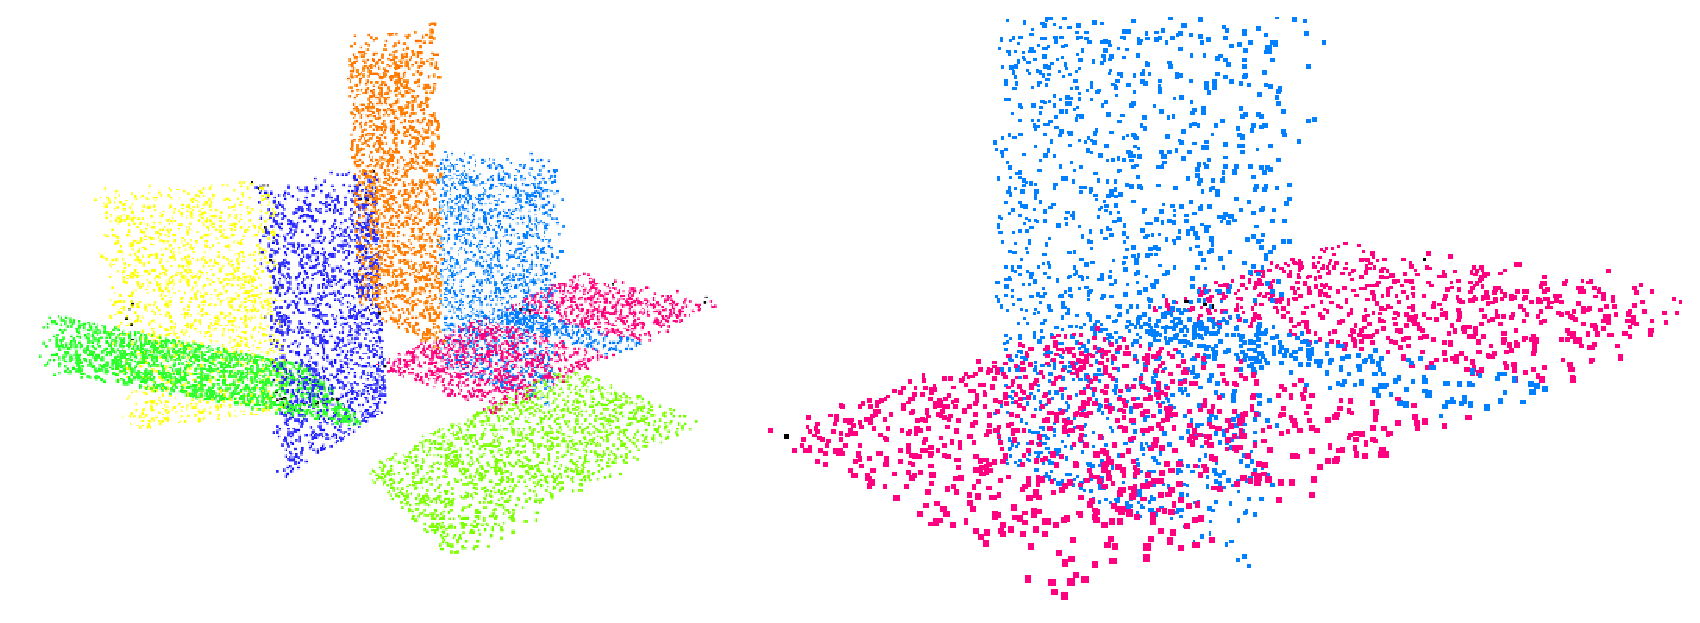
\includegraphics[width=\textwidth]{figures/test-chyba-1}
\caption{Ukázka testovací segmentace, která je v tabulce \ref{table:test1-gen} označena jako 7-0. Vlevo je zobrazena výsledná segmentace, vpravo je detail na popsanou chybu při segmentaci.}
\label{fig:test-chyba-1}
\end{center}
\end{figure}

Pro ilustraci přidávám ještě jednu ukázku testovací segmentace, na obrázku \ref{fig:test-6-0} je mračno označené v tabulce jako 6-0.

\begin{figure}[H]
\begin{center}
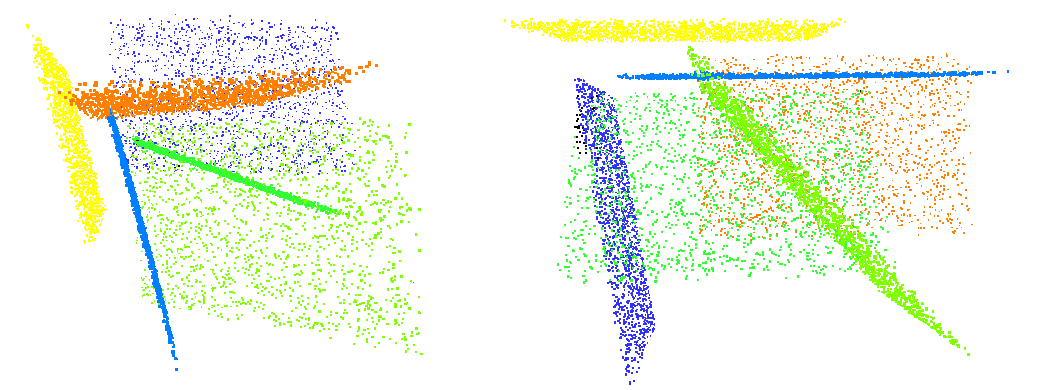
\includegraphics[width=\textwidth]{figures/test-6-0}
\caption{Ukázka testovací segmentace, která je v tabulce \ref{table:test1-gen} označena jako 6-0. Jedná se o stejné mračno z různých úhlů.}
\label{fig:test-6-0}
\end{center}
\end{figure}

Vzhledem k tomu, že ve všech testovacích případech byly nalezeny všechny roviny, algoritmus rozhodně funguje správně. Zároveň ve všech případech bylo segmentováno více jak 99,3\% bodů. Ve většině případů byl počet špatně přiřazených bodů velmi malý, kromě dvou již zmiňovaných případů.

\newpage
\section{Testování kvality algoritmů na reálných datech}

V této části jsou otestovány oba algoritmy na reálných mračnech bodů, které jsem měl k dispozici. Testován je jednak výkon algoritmů a dále také kvalita samotné segmentace. Všechna testovaná mračna jsou k dispozici na přiloženém CD, stejně tak CD obsahuje výsledky všech segmentací v této kapitole. Výsledky segmentace budou vždy shrnuté v tabulce, kde bude mít každý test unikátní označení. Soubory na CD budou pro přehlednost označeny stejně, takže vždy půjde jednoduše přiřadit soubor na CD k datům popisovaným v textu.

Během testování algoritmu bude nejprve na dvou různých mračnech bodů ukázáno, jaký vliv mají parametry segmentace na dobu a výstup segmentace. Poté bude ukázáno, jaký je vliv parametrů segmentace na dobu běhu algoritmu a jaká je spotřeba paměti algoritum. Dále budou v kapitole ukázány výsledky segmentace z dalších mračen bodů, zde už budou ukázány pouze výsledky s nejlepšími parametry.

\subsection{Vliv parametrů na výslednou segmentaci}
\label{sub:vliv-param}

Pro ukázku vlivu parametrů na výslednou segmentaci jsem vybral dvě různá mračna (viz Obr. \ref{fig:dum-stodulky}). První mračno je označeno jako \uv{dům 2}, toto mračno je složeno z 723695 bodů a obsahuje 3 velké roviny. Oproti tomu druhé mračno \uv{stodůlky} obsahuje více jak 10 rovin a skládá se ze 604411 bodů. Obě mračna reprezentují část budovy, ale zároveň obsahují poměrně velké množství bodů, které do žádné roviny nepatří.

\begin{figure}[H]
\begin{center}
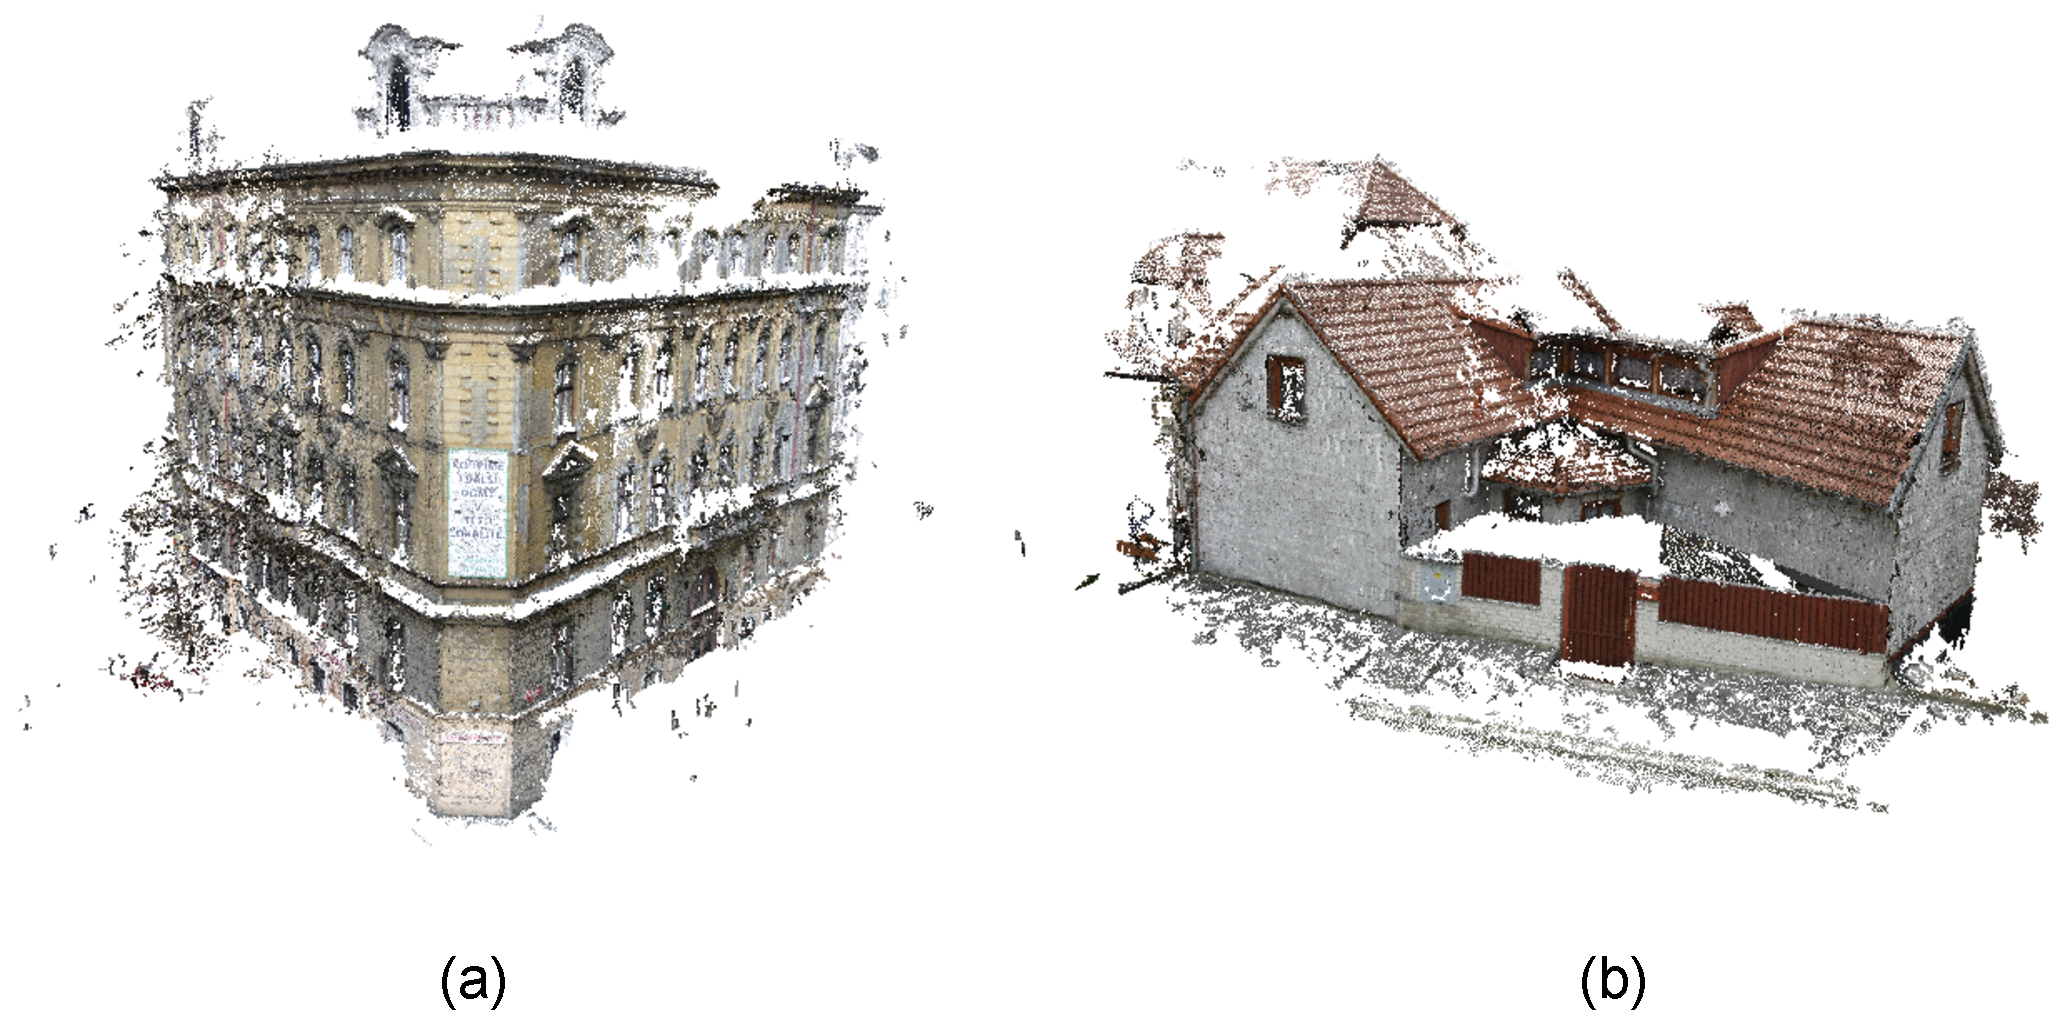
\includegraphics[width=\textwidth]{figures/dum2-stodulky}
\caption{Ukázka mračna bodů dům 2 (a) a stodůlky (b).}
\label{fig:dum-stodulky}
\end{center}
\end{figure}

Cílem tohoto testu je ukázat, jak jednotlivé parametry ovlivňují výslednou segmentaci. Cílem tedy není docílit co nejlepší segmentace, toho se bude týkat až další část testování. Nejprve bude testováno mračno dům 2. Tabulka \ref{table:test2-param-d2} ukazuje výsledky testování mračna. Na obrázku \ref{fig:test-dum2-seg} jsou zobrazeny některé z výsledků tohoto testování.

\begin{table}[H]
\begin{center}
\begin{tabular}{|r|r|r|r|r|r|}
\hline
\multicolumn{1}{|c|}{test} & \multicolumn{1}{c|}{P1} & \multicolumn{1}{c|}{P2} & \multicolumn{1}{c|}{P3} & \multicolumn{1}{c|}{seg. bodů} & \multicolumn{1}{c|}{segmentů} \\ \hline
d2-0.00 & 10 & 1 & 1 & 25,68\% & 1 \\ \hline
d2-0.01 & 10 & 1 & 10 & 31,37\% & 1 \\ \hline
d2-0.02 & 10 & 2 & 1 & 54,53\% & 3 \\ \hline
d2-0.03 & 10 & 2 & 2 & 56,65\% & 3 \\ \hline
d2-0.04 & 10 & 2 & 3 & 60,09\% & 3 \\ \hline
d2-0.05 & 10 & 2 & 5 & 63,00\% & 3 \\ \hline
d2-0.06 & 10 & 2 & 10 & 63,36\% & 3 \\ \hline
d2-0.07 & 10 & 2 & 20 & 63,79\% & 3 \\ \hline
d2-0.08 & 10 & 3 & 1 & 53,75\% & 3 \\ \hline
d2-0.09 & 10 & 4 & 1 & 53,71\% & 3 \\ \hline
d2-0.10 & 10 & 5 & 1 & 53,75\% & 3 \\ \hline
d2-0.11 & 10 & 10 & 1 & 57,00\% & 4 \\ \hline
d2-0.12 & 20 & 2 & 1 & 54,79\% & 3 \\ \hline
d2-0.13 & 40 & 2 & 1 & 56,91\% & 3 \\ \hline
d2-0.14 & 80 & 2 & 1 & 61,12\% & 4 \\ \hline
d2-0.15 & 120 & 2 & 1 & 54,38\% & 4 \\ \hline
\end{tabular}
\caption{Tabulka zobrazuje výsledky testování algoritmu na mračnu dům 2 při různých parametrech. Paramtery jsou popsány v příloze \ref{chap:zkratky}.} 
\label{table:test2-param-d2}
\end{center}
\end{table}

Protože mračno obsahuje poměrně přesné roviny bez větších chyb a nerovností, pro testování stačilo i velmi malé okolí, segmentace fungovala správně již při okolí 10 bodů. Z tabulky by mělo být patrné, že pokud byl zadán parametr pro klastrování 1, byla tato hodnota příliš nízká a byl rozpoznán pouze jeden segment. Nicméně při zvýšení této hodnoty na 2 byly nalezeny již všechny tři očekávané segmenty. Při této hodnotě jsem dále měnil parametr určující kvalitu klastrování. Podle očekávání při zvýšení tohoto parametru narůstal počet bodů obsažených v segmentech. Při zvýšení parametru z 1 na 20 bylo  segmentováno o 9\% bodů více. Jak je ale z tabulky patrné, největší nárůst přidaných bodů byl při postupném zvyšování parametru od 1 do 5, následné zvyšování parametru již nemělo na segmentaci výrazný vliv. Pro běžné podmínky tedy nemá smysl tento parametr nastavovat na vyšší hodnotu než 10. V dalších testech byl zvyšován parametr klastrování (jde o data označená d2-0.8 - d2-0.11). Z tabulky je patrné, že se při počátečním zvyšování parametru výsledná segmentace výrazně neměnila. To je logické, protože při zvyšování parametru se snižovala hranice pro vyhledávání vrcholů v akumulátorovém poli, ale protože body ze tří velkých rovin vytvořily tři vysoké vrcholy, byly nalezeny stejně při všech těchto hodnotách parametru. Až při hodnotě 10 byl práh při prohledávání pole tak nízko, že našel nějaká zbytková data tvořící rovinu. Tato situace bude popsána v následujícím odstavci.

\begin{figure}[ht]
\begin{center}
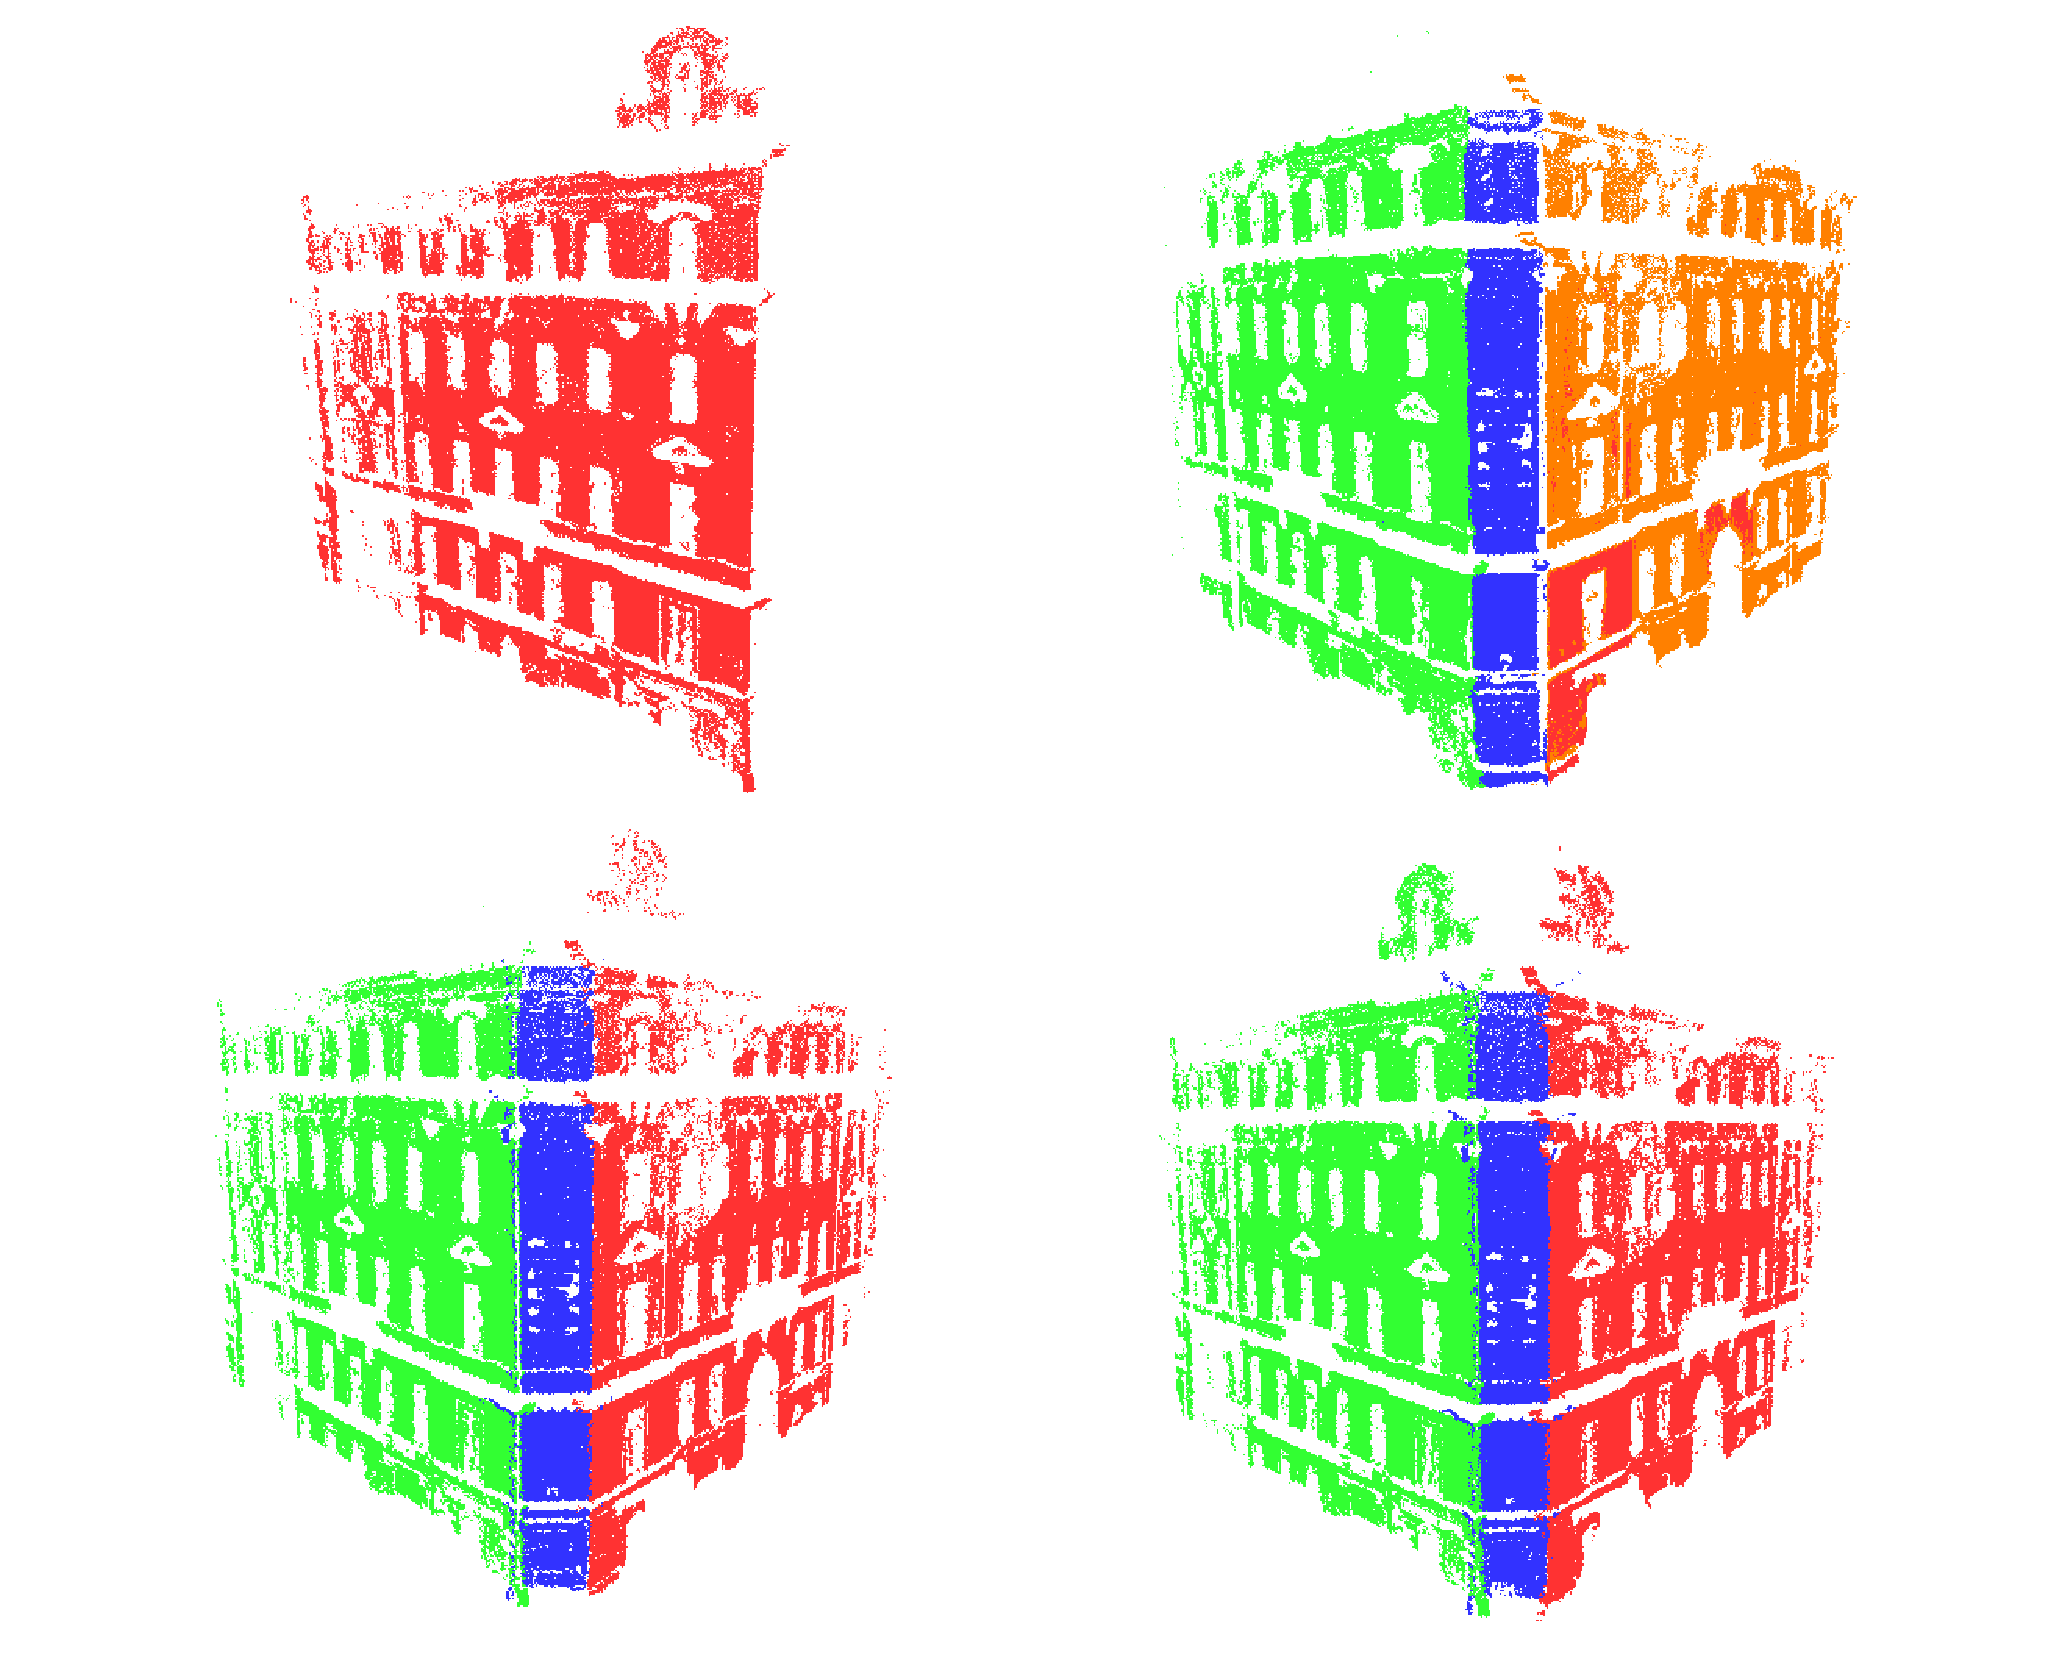
\includegraphics[width=\textwidth]{figures/test-dum2-seg}
\caption{Ukázka vybraných mračen bodů z testování. Obrázky odpovídají značení v tabulce: (a) d2-0.01, (b) d2-0.14, (c) d2-0.02, (d) d2-0.07.}
\label{fig:test-dum2-seg}
\end{center}
\end{figure}

V posledních 4 řádcích tabulky byla postupně zvyšována velikost okolí. Zvýšení na 20 a 40 bodů nemělo na segmentaci žádný výrazný vliv, segmentace byla jen o málo přesnější, což se projevilo ve zvýšném počtu segmentovaných bodů o několik procent. Při dalším zvyšování velikosti okolí však bylo nalezeno více segmentů, než se očekávalo. Toto je paradoxně způsobeno tím, že parametry bodů byly při větším okolí vypočteny přesněji. Konkrétní problém je v tom, že body tvořící nejvyšší buňku vrcholu jsou velmi přesně v rovině. Na základě těchto bodů je vypočteno RMS, které v následném klastrování určuje \uv{tloušťku} roviny, tedy přesněji vzdálenost, v jaké může bod od roviny být, aby byl ještě do segmentu zahrnut. Pokud je ale toto RMS malé (protože původní body byly  velmi přesně v rovině), jsou vybrány pouze ty nejpřesnější body. To má za následek, že v akumulátorovém poli zůstanou body, které tvoří rovinu, akorát méně přesnou. Bodů je však stále ještě dostatek, aby byl vrchol v akumulátorovém poli výrazný. Tím pádem je vrchol v další iteraci prohledávání akumulátorového pole detekován a z bodů je vytvořen nový segment. Výsledkem je tedy to, že z jedné roviny jsou vytvořeny dva segmenty. První segment obsahuje nejpřesnější body z této roviny, druhý obsahuje zbylé, méně přesné body. Tento problém se při klastrování velmi těžko detekuje. Je založen na faktu, že vypočtené RMS je malé. Nicméně v rámci algoritmu neexistuje žádná referenční hodnota, podle které by šlo rozhodnout, že RMS je malé. Proto se mi tento problém nepodařilo detekovat během klastrování. Řešením by mohla být dodatečná detekce po klastrování, kdy by se zjišťovalo, zda jednotlivé segmenty nereprezentují stejnou rovinu. Řešení ani detekce tohoto problému nejsou v této práci implementovány. Jako možné řešení se nabízí sloučení segmentů ležících v jedné rovině. Toto by šlo provést až na základě výseldků segmentace bez nutnosti zashovat do hotového algoritmu.

Celkově lze tedy říci, že algoritmus je poměrně robustní pro mračno s malým počtem velkých rovin. Není výrazně závislý na zadané velikosti okolí, až při větších okolí nastává výše popsaný problém. Zároveň není algoritmus příliš závislý na parametru klastrování, fungoval správně od hodnoty 2 do hodnoty 10. Při této hodnotě však již byl nalezen jeden segment navíc. I v tomto případě byly 2 segmenty součástí jedné roviny jako ve výše popsané situaci. Příčina zde ale byla trochu jiná. Protože kvalita segmentů byla nastavena na 1, po vybrání 3 největších segmentů stále v akumulátorovém poli zbyly zbytky těchto rovin, které nebyly segmentovány. A protože byl parametr klastrování nastaven na 10, práh pro prohledávání pole byl tak nízký, že tyto zbytky byly detekovány jako segment. Řešením této situace je snížit parametr klastrování nebo zvýšit kvalitu klastrování. 

Za zmínku ještě stojí poměrně nízký počet segmentovaných bodů, který byl v nejlepším případě necelých 64\% bodů. To je dáno tím, že mračno obsahuje poměrně velký počet bodů, které v daných rovinách neleží (viz Obr. \ref{fig:dum-stodulky} (a)).

Pro druhou ukázku vlivu parametrů na segmentaci použiji mračno stodůlky. Na tomto mračnu bude ukázáno, jaký vliv má parametr klastování na výslednou segmentaci. Výsledky testování jsou uvedeny v tabulce \ref{table:test3-klastr}.

\begin{table}[ht]
\begin{center}
\begin{tabular}{|r|r|r|r|r|r|}
\hline
\multicolumn{1}{|c|}{\textbf{test}} & \multicolumn{1}{c|}{\textbf{P1}} & \multicolumn{1}{c|}{\textbf{P2}} & \multicolumn{1}{c|}{\textbf{P3}} & \multicolumn{1}{c|}{\textbf{seg. bodů}} & \multicolumn{1}{c|}{\textbf{segmentů}} \\ \hline
st-0.00 & 30 & 1 & 5 & 37,42\% & 3 \\ \hline
st-0.01 & 30 & 3 & 5 & 55,24\% & 6 \\ \hline
st-0.02 & 30 & 4 & 5 & 61,33\% & 8 \\ \hline
st-0.03 & 30 & 5 & 5 & 62,51\% & 9 \\ \hline
st-0.04 & 30 & 6/7 & 5 & 65,42\% & 11 \\ \hline
st-0.05 & 30 & 8 & 5 & 66,10\% & 12 \\ \hline
st-0.06 & 30 & 9/10 & 5 & 66,40\% & 13 \\ \hline
st-0.07 & 30 & 11 & 5 & 66,50\% & 14 \\ \hline
\end{tabular}
\caption{Tabulka zobrazuje výsledky testování algoritmu na mračnu stodůly při různých parametrech klastrování. Paramtery jsou popsány v příloze \ref{chap:zkratky}.} 
\label{table:test3-klastr}
\end{center}
\end{table}

Z tabulky je jasně vidět, že při zvyšování parametru klastrování postupně přibývá počet nalezených segmentů. Nejprve jsou nalezeny segmenty s největším počtem bodů, případně segmenty s body, které jsou velmi přesně v rovině. Při zvyšování jsou postupně nacházeny menší nebo méně kvalitní roviny. V tabulce můžeme vidět, že při zvyšování parametru až na hodnotu 8 jsou nacházeny segmenty, které řádově přidávají aspoň procenta bodů z celkového mračna. Při dalším zvyšování už jsou nalezeny pouze velmi malé segmenty, dá se tedy očekávat, že při vyšší hodnotě parametru jak 8 už nebudou nalezeny žádné významné segmenty ale pouze již nějaké velmi malé segmenty, případně budou chybně segmentovány zbytky již nalezených segmentů, jak bylo popsáno dříve v této kapitole. Na obrázku \ref{fig:test-stodulky-seg} jsou zobrazeny ukázky některých testovacích segmentací.

\begin{figure}[ht]
\begin{center}
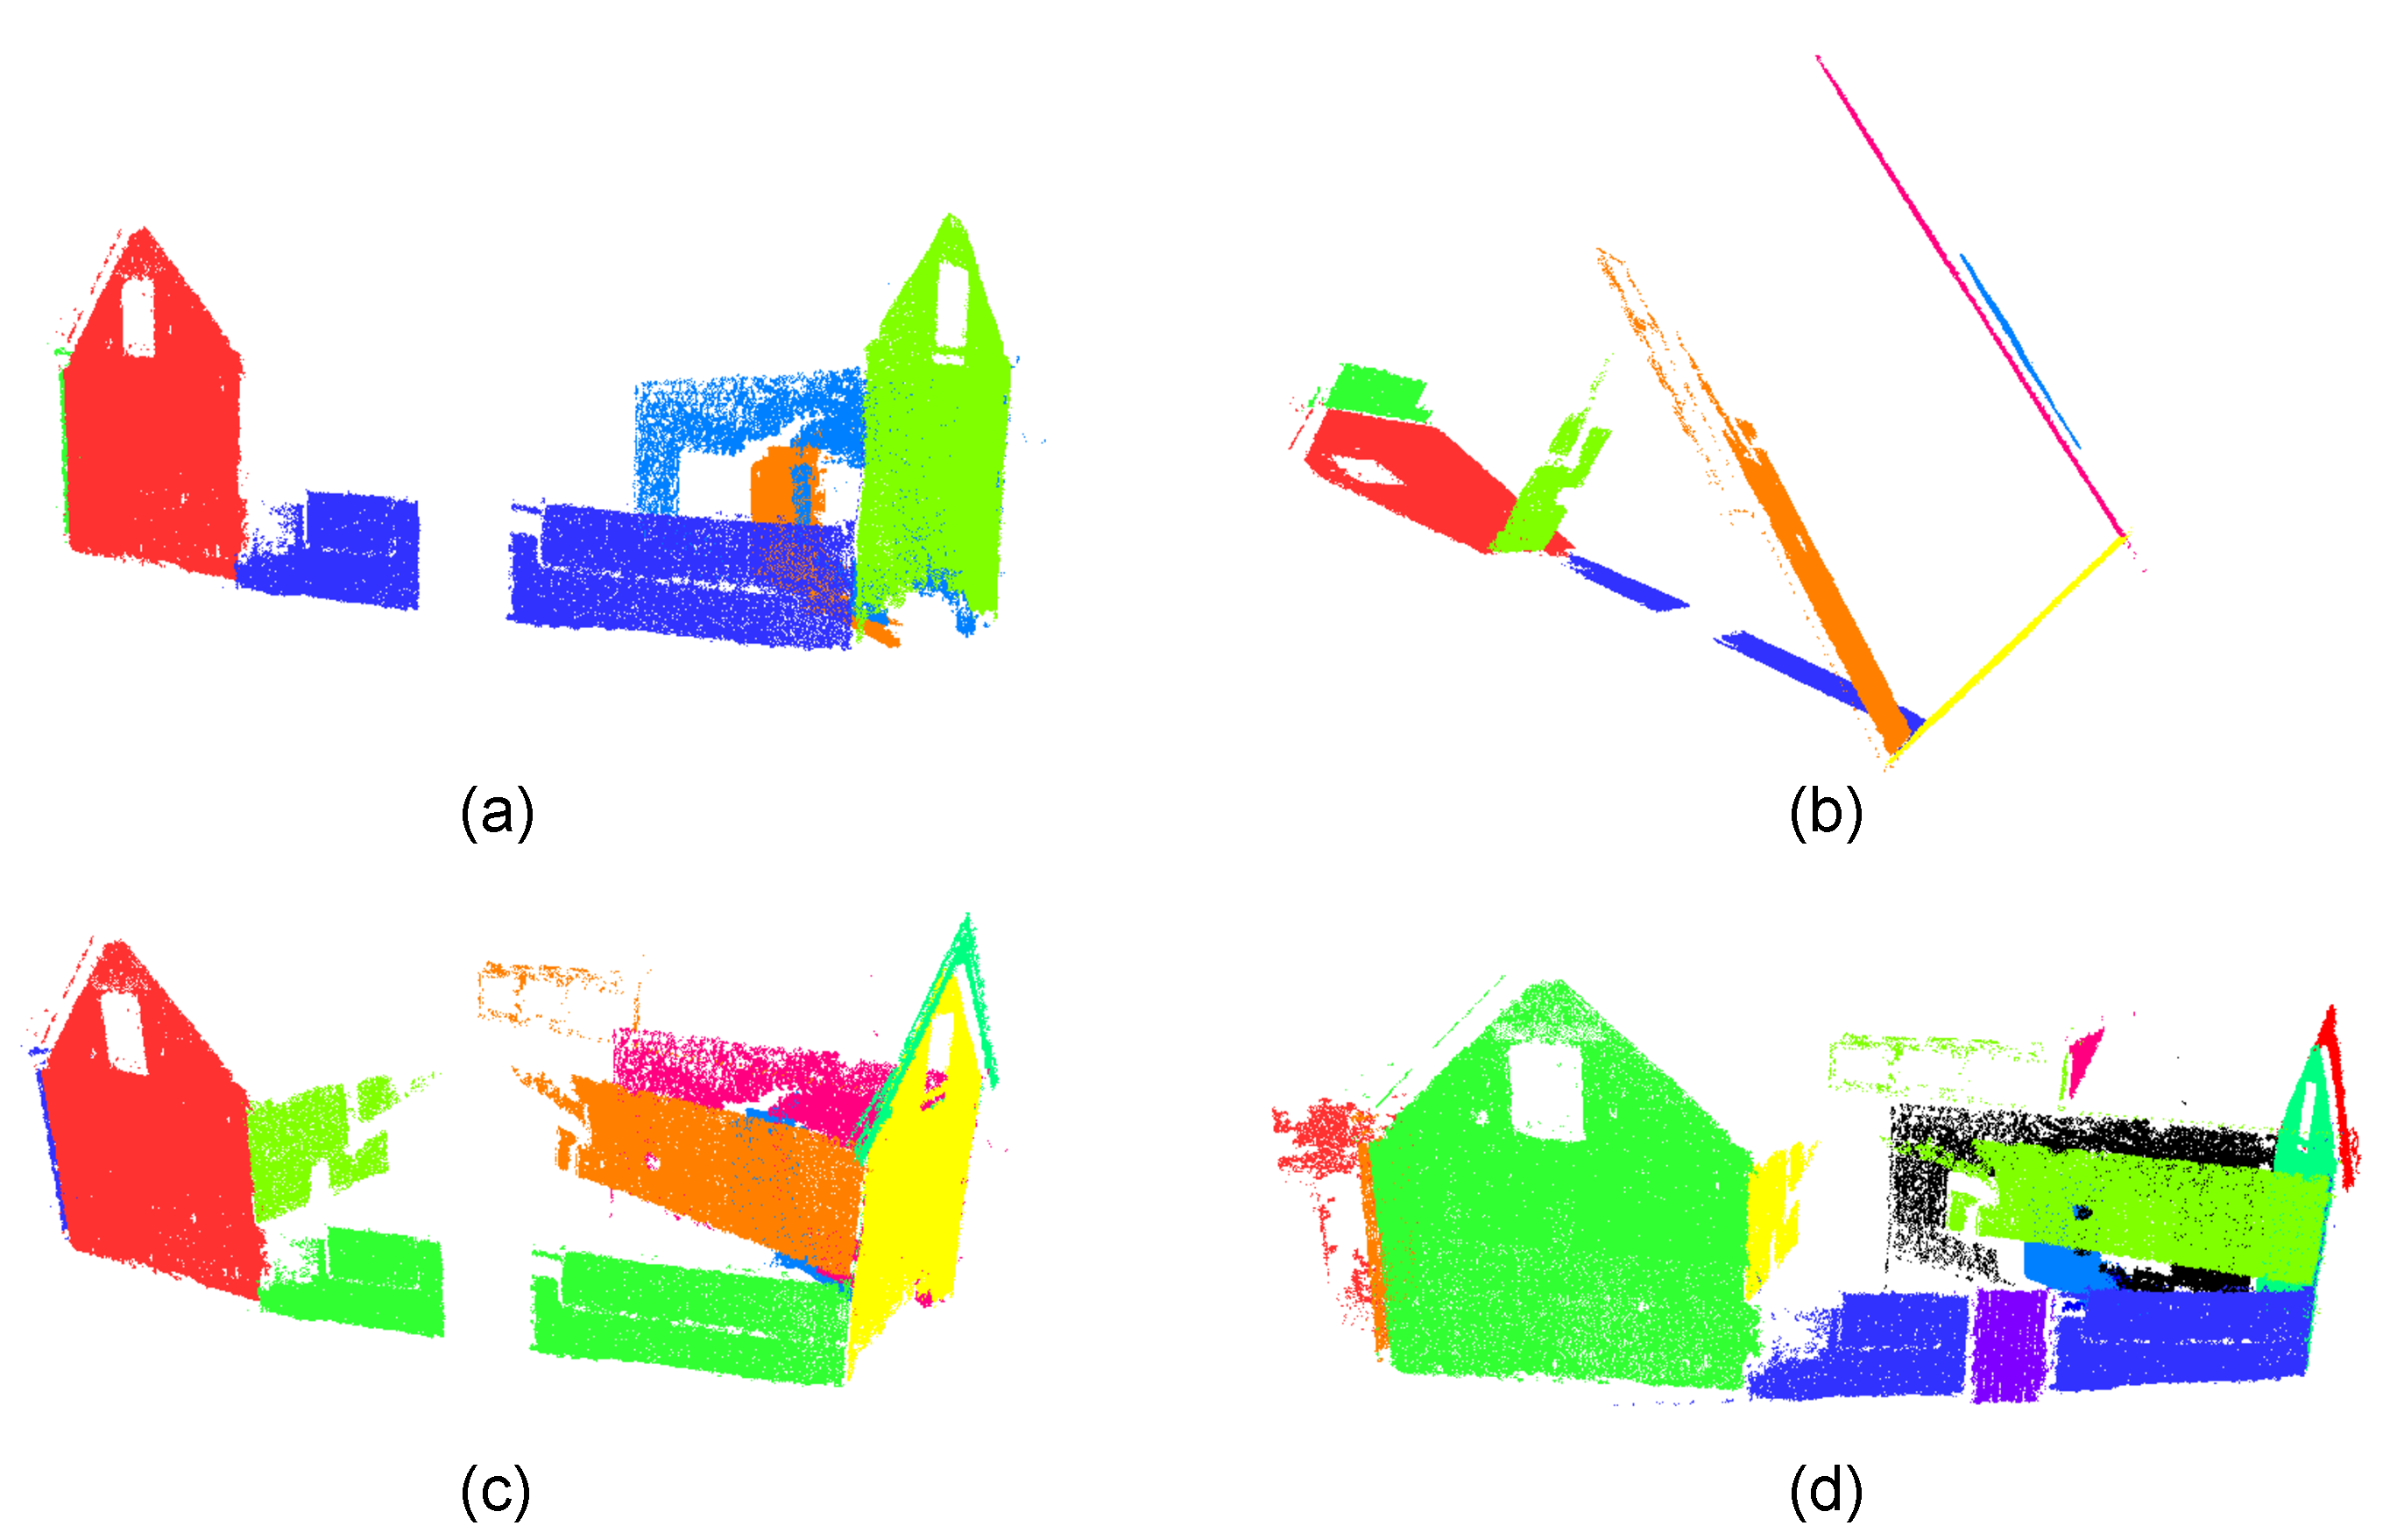
\includegraphics[width=\textwidth]{figures/test-stodulky-seg}
\caption{Ukázka vybraných mračen bodů z testování z různých pohledů. Obrázky odpovídají značení v tabulce: (a) st-0.01, (b) st-0.02, (c) st-0.03, (d) st-0.06.}
\label{fig:test-stodulky-seg}
\end{center}
\end{figure}

Z obrázků je patrné, že algoritmus nedetekoval dvě střechy, které jsou rovinné a obsahují poměrně velké množství bodů (viz Obr. \ref{fig:dum-stodulky}). Tento problém nastal proto, že na velkém měřítku střechy vypadají rovně, ale jejich povrch je ve skutečnosti hodně hrbolatý, na malém měřítku tedy není dostatečně rovný. Parametry jednotlivých bodů na střeše jsou tím pádem poměrně rozdílné a body ze střechy nevytvoří v akumulátorovém poli dostatečně výrazný vrchol. Aby byl algoritmus schopen střechy detekovat, je potřeba použít výrazně větší okolí, než 30 bodů, které bylo použito v tomto testu. Nicméně jak jsem zmiňoval na začátku této sekce, cílem těchto dvou testů bylo ukázat, jak parametry ovlivňují segmentaci, nikoliv získat při segmentaci co nejlepší výsledky. Na to dojde v pozdější části této kapitoly.


\newpage
\subsection{Testování časové a paměťové složitosti algoritmu}

Protože je algoritmus poměrně komplikovaný a používá složitější datové struktury, nejde příliš jednoduše odhadnou asymptotickou složitost algoritmu. Proto jsem pouze měřil paměť za běhu programu a dobu běhu programu. Pro sledování alokované paměti jsem použil program VisualVM verze 1.3.4. Nejprve jsem testoval  segmentaci mračna bodů dům 2 (723695 bodů) s velikostí okolí 80 bodů, parametrem klastrování 1 a kvalitou klastrování 10. Výsledky měření jsou zachyceny v grafu na obrázku \ref{fig:memory-graph-all}.

\begin{figure}[ht]
\begin{center}
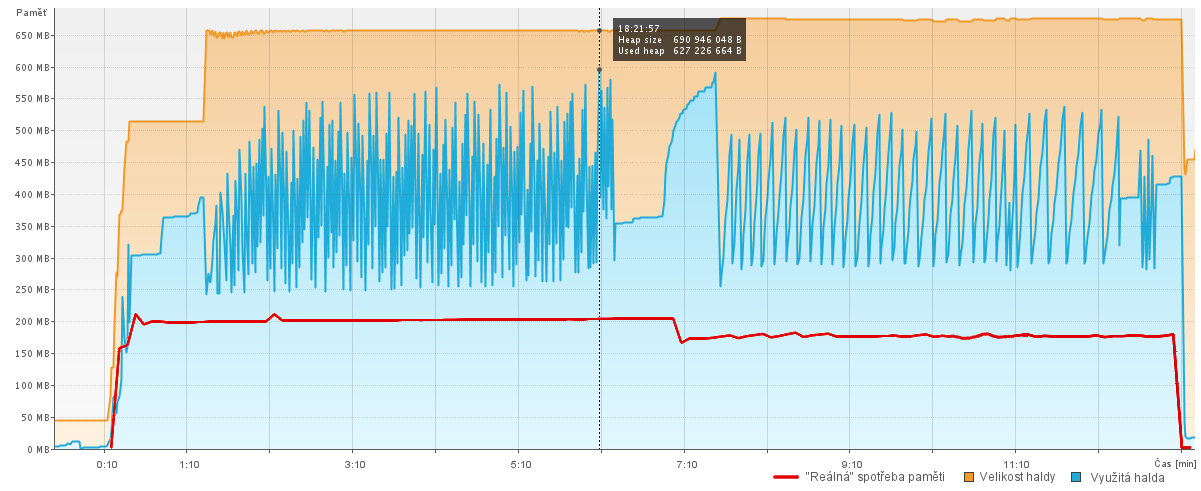
\includegraphics[width=\textwidth]{figures/memory-graph-all}
\caption{Graf zobrazující velikost využité paměti za běhu algoritmu.}
\label{fig:memory-graph-all}
\end{center}
\end{figure}

Graf zobrazuje velikost alokované haldy a její reálné využití za běhu aplikace. Detail začátku grafu s popisem je zobrazen na obrázku \ref{fig:memory-graf1}. Graf je ovšem z jiného měření při stejných datech, takže se jeho hodnoty mohou nepatrně lišit. 

\begin{figure}[ht]
\begin{center}
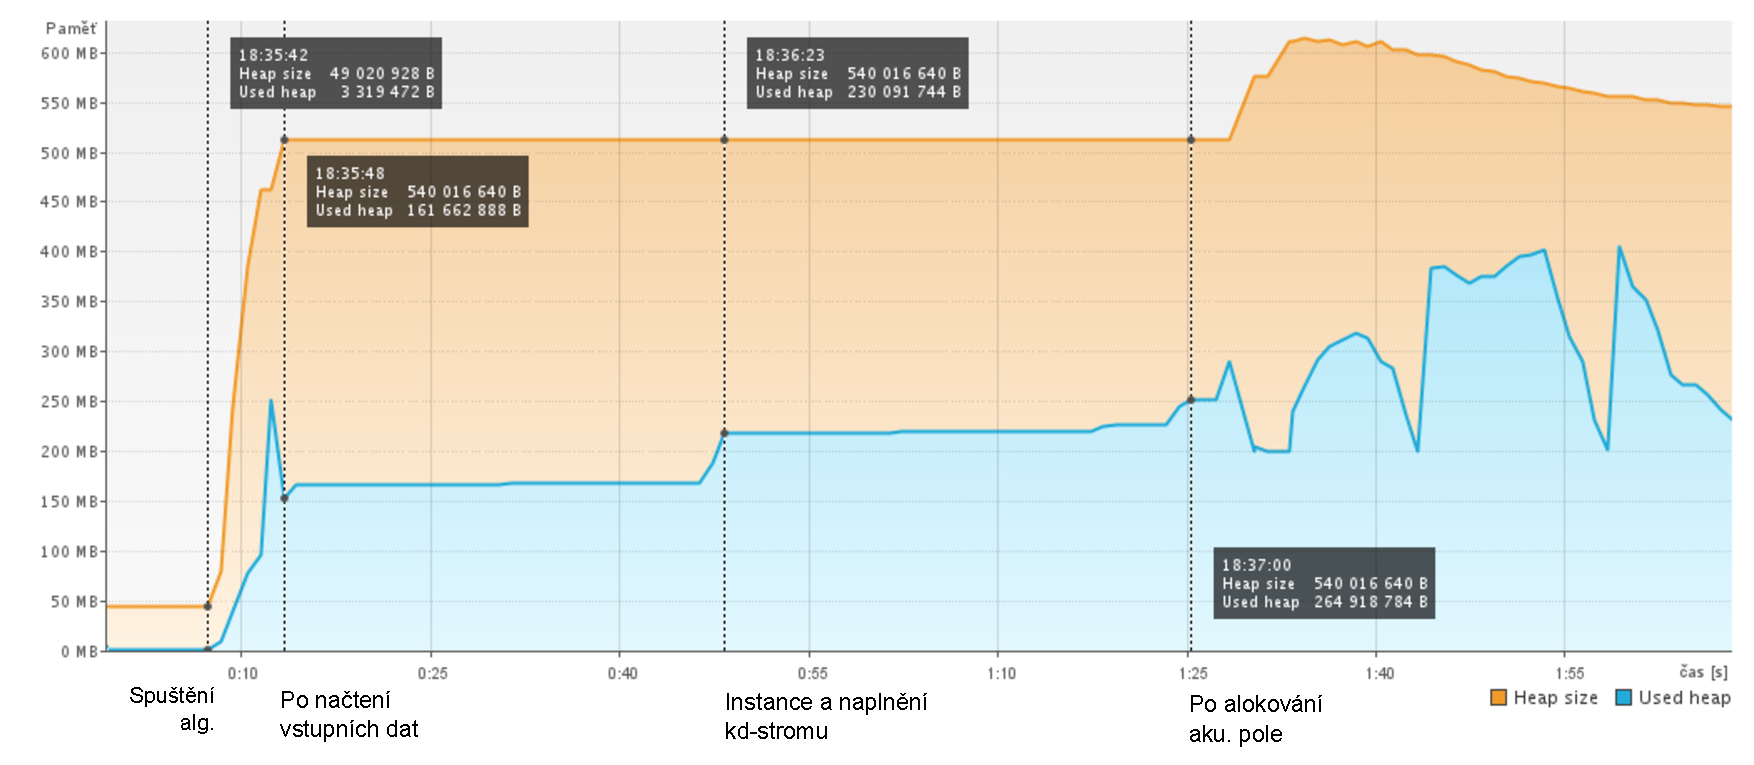
\includegraphics[width=\textwidth]{figures/memory-graf1}
\caption{Graf zobrazující velikost využité paměti při inicializaci algoritmu.}
\label{fig:memory-graf1}
\end{center}
\end{figure}

Důležité hodnoty v prvním grafu jsou v čase 1:30, kdy začal výpočet parametrů a dále čas 6:50, kdy začalo vybírání bodů z akumulátorového pole. To skončilo v čase 12:30, poté byl vyexportován výstup a v čase 13:00 byl algoritmus ukončen. Protože se během výpočtu parametrů bodů a při vybírání bodů z akumulátorového pole používá velké množství krátkodobých instancí, je výsledný graf velmi ovlivněn chováním garbage collectoru. Proto jsem provedl druhé měření, kdy jsem před každým odečítáním paměti explicitně volal garbage collector - to tedy odpovídá hodnotě paměti, kterou zabírají \uv{živé} instance. Toto měření je v grafu zakreslené červenou křivkou. Protože šlo o dvě různá měření, grafy se mohou na ose x vzájemně lišit, nicméně maximálně o několik vteřin.

Z grafů by mělo být patrné, že velikost potřebné paměti je nejvíce závislá na množství vstupních dat, algoritmus poté potřebuje další paměť na vytvoření kd-stromu a alokaci akumulátorového pole, ale dále za běhu již nealokuje žádné výrazné množství paměti. Na paměťových nárocích by se tedy neměly výrazně projevit ani použité parametry. Na obrázku \ref{fig:memory-graf2} je graf, který zobrazuje využitou paměť při segmentaci mračna stodůlky s různými parametry. Před každým odebraným vzorkem paměti byl volán garbage collector. První test zobrazuje segmentaci s velikostí okolí 20, parametrem klastrování 8 a kvalitou klastrování 1, druhý test je proveden s parametry 80, 8 a 10. Z grafu je patrné, že alokovaná paměť je v obou případech stejná. Pokles paměti v prostřední čísti grafu odpovídá ukončení ukládání bodů do akumulátorového pole a začátku vybírání segmentů.

\begin{figure}[ht]
\begin{center}
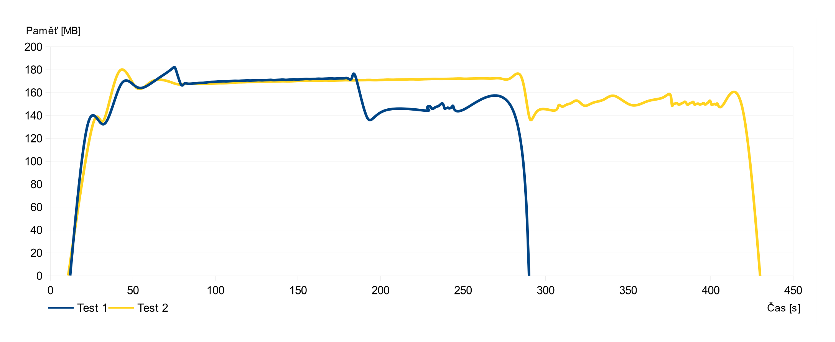
\includegraphics[width=\textwidth]{figures/memory-graf2}
\caption{Graf zobrazující velikost využité paměti při spuštění algoritmu s různými parametry.}
\label{fig:memory-graf2}
\end{center}
\end{figure}

Z grafu je také jasně vidět, že hodnota parametrů ovlivňuje zejména dobu běhu algoritmu. To však není žádné překvapení, důvody jsou popsané v kapitole \ref{chap:implementace}. Následující testování se tedy bude věnovat měření doby běhu algoritmu při různých vstupních parametrech. Zajímavé bude také srovnání, jaká část z celkové doby běhu algoritmu odpovídá vyhledávání okolí v kd-stromu a počítání SVD dekompozice při prokládání roviny množinou bodů. Testování proběhlo pouze na mračnu stodůlky. Výsledky testování rychlosti algoritmu jsou shrnuty v tabulce \ref{table:test-cas}.

\begin{table}[ht]
\resizebox{\textwidth}{!} {
\begin{tabular}{|r|r|r|r|r|r|r|r|r|r|r|r|r|}
\hline
\multicolumn{1}{|l|}{} & \multicolumn{ 3}{c|}{\textbf{Parametry}} & \multicolumn{ 9}{c|}{\textbf{Čas [sec]}} \\ \hline
\multicolumn{1}{|c|}{\textbf{test}} & \multicolumn{1}{c|}{\textbf{P1}} & \multicolumn{1}{c|}{\textbf{P2}} & \multicolumn{1}{c|}{\textbf{P3}} & \multicolumn{1}{c|}{\textbf{celkem}} & \multicolumn{ 2}{c|}{\textbf{ukládání do aku.}} & \multicolumn{ 2}{c|}{\textbf{vybírání z aku.}} & \multicolumn{ 2}{c|}{\textbf{kd-strom}} & \multicolumn{ 2}{c|}{\textbf{SVD}} \\ \hline
\textbf{1} & 10 & 8 & 1 & 64,34 & 55,48 & 86,24\% & 8,21 & 12,76\% & 12,82 & 19,93\% & 17,76 & 27,60\% \\ \hline
\textbf{2} & 10 & 8 & 2 & 66,97 & 55,48 & 82,85\% & 10,84 & 16,18\% & 12,82 & 19,15\% & 17,82 & 26,61\% \\ \hline
\textbf{3} & 10 & 8 & 3 & 73,48 & 55,48 & 75,51\% & 18,00 & 24,49\% & 12,82 & 17,45\% & 17,90 & 24,36\% \\ \hline
\textbf{4} & 10 & 8 & 5 & 85,70 & 55,48 & 64,74\% & 30,22 & 35,26\% & 12,82 & 14,96\% & 17,91 & 20,90\% \\ \hline
\textbf{5} & 10 & 8 & 8 & 107,66 & 55,48 & 51,54\% & 52,17 & 48,46\% & 12,82 & 11,91\% & 17,92 & 16,64\% \\ \hline
\textbf{6} & 10 & 8 & 10 & 115,26 & 55,48 & 48,14\% & 59,78 & 51,86\% & 12,82 & 11,12\% & 17,93 & 15,56\% \\ \hline
\textbf{7} & 10 & 8 & 20 & 173,47 & 55,48 & 31,99\% & 117,98 & 68,01\% & 12,82 & 7,39\% & 17,94 & 10,34\% \\ \hline
\textbf{8} & 20 & 8 & 5 & 93,84 & 71,50 & 76,19\% & 22,34 & 23,81\% & 18,07 & 19,26\% & 23,58 & 25,13\% \\ \hline
\textbf{9} & 30 & 8 & 5 & 123,38 & 86,55 & 70,15\% & 36,83 & 29,85\% & 23,78 & 19,27\% & 26,42 & 21,41\% \\ \hline
\textbf{10} & 50 & 8 & 5 & 172,05 & 119,14 & 69,25\% & 52,91 & 30,75\% & 34,93 & 20,30\% & 37,08 & 21,55\% \\ \hline
\textbf{11} & 80 & 8 & 5 & 225,54 & 172,19 & 76,34\% & 53,35 & 23,66\% & 54,56 & 24,19\% & 49,84 & 22,10\% \\ \hline
\textbf{12} & 100 & 8 & 5 & 281,07 & 224,82 & 79,99\% & 56,24 & 20,01\% & 71,51 & 25,44\% & 72,01 & 25,62\% \\ \hline
\textbf{13} & 40 & 1 & 5 & 109,90 & 102,05 & 92,86\% & 7,85 & 7,69\% & 28,53 & 27,96\% & 31,17 & 30,54\% \\ \hline
\textbf{14} & 40 & 2 & 5 & 128,48 & 102,05 & 79,43\% & 26,43 & 20,57\% & 28,53 & 22,21\% & 31,19 & 24,27\% \\ \hline
\textbf{15} & 40 & 3 & 5 & 127,64 & 102,05 & 79,95\% & 25,59 & 20,05\% & 28,53 & 22,35\% & 31,21 & 24,45\% \\ \hline
\textbf{16} & 40 & 4 & 5 & 131,66 & 102,05 & 77,51\% & 29,62 & 22,49\% & 28,53 & 21,67\% & 32,36 & 24,58\% \\ \hline
\textbf{17} & 40 & 6 & 5 & 134,90 & 102,05 & 75,65\% & 32,85 & 24,35\% & 28,53 & 21,15\% & 33,35 & 24,72\% \\ \hline
\textbf{18} & 40 & 8 & 5 & 138,28 & 102,05 & 73,80\% & 36,23 & 26,20\% & 28,53 & 20,63\% & 33,37 & 24,13\% \\ \hline
\end{tabular}
}
\caption{Tabulka zobrazuje výsledky testování rychlosti algoritmu v závislosti na zadaných parametrech. Paramtery jsou popsány v příloze \ref{chap:zkratky}.} 
\label{table:test-cas}
\end{table}

\begin{figure}[H]
\begin{center}
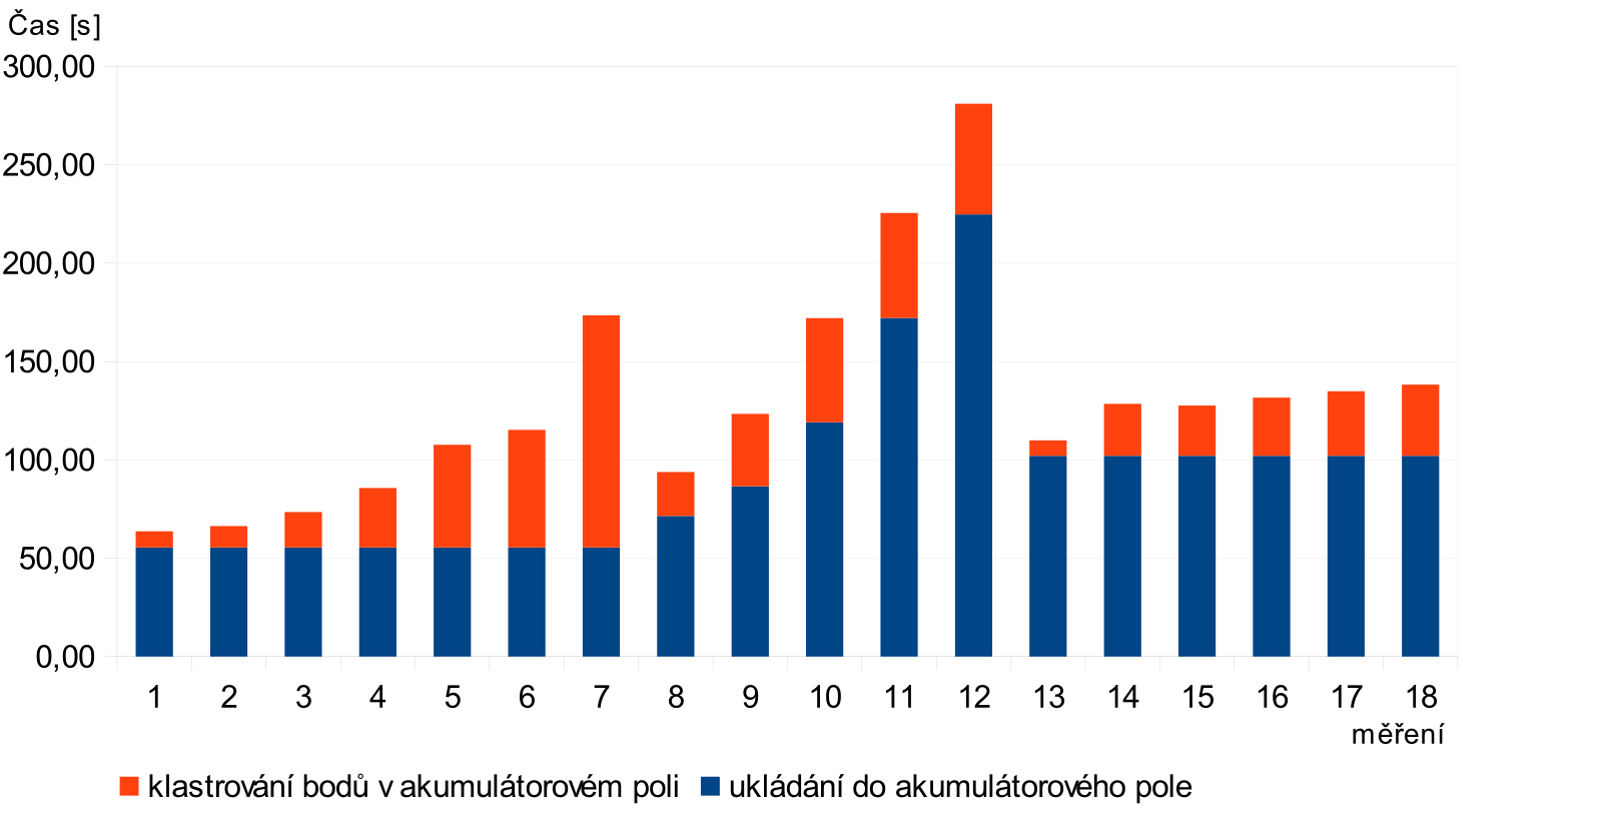
\includegraphics[width=\textwidth]{figures/graf-test-cas}
\caption{Graf zobrazující dobu běhu algoritmu v závislosti na zadaných parametrech. V grafu jsou znázorněna data z tabulky \ref{table:test-cas}.}
\label{fig:graf-test-cas}
\end{center}
\end{figure}

Některá data z tabulky jsou zachycena v grafu na obrázku \ref{fig:graf-test-cas}, konkrétně je v grafu znázorněn celkový čas segmentace a zároveň část, kterou zabralo ukládání bodů do akumulátorového pole a poté klastrování bodů v poli. Prvních 7 řádků v tabulce (tedy prvních 7 sloupců v grafu) zobrazuje změnu doby běhu algoritmu při zvyšování kvality klastrování. Jak se dá očekávat, zvýšení parametru zvyšuje dobu trvání klastrování bodů v poli. Ukládání do pole není ovlivněno vůbec (bylo provedenou pouze jednou, proto jsou u všech měření hodnoty totožné). V následujících 5ti měřeních je zvyšována velikost okolí bodu při ukládání bodů do akumulátorového pole. Opět se podle očekávání zvyšuje doba běhu se zvětšováním okolí. Doba klastrování se liší jen podle toho, jaká byla kvalita nalezených segmentů. V posledních 6ti měřeních je měněn parametr klastrování. Z naměřených dat je zřetelné, že tento parametr nemá na dobu běhu zásadní vliv. Mění se pouze doba klastrování bodů v akumulátorovém poli, která je závislá na počtu nalezených segmentů \footnote{Tato hodnota zde není uvedena, ale je totožná s daty uvedenými v tabulce \ref{table:test3-klastr}}.


\subsection{Výsledky segmentace dodaných dat}
V této části budou ukázány nejlepší výsledky segmentace všech dodaných testovacích mračen bodů. U každého testu segmentace je uvedena tabulka s výsledky. Tabulka zobrazuje, kolik bodů z celkového počtu bylo segmentováno. Dále je v tabulce uvedeno, kolik segmentů bylo nalezeno, kolik segmentů bylo očekáváno\footnote{Tato hodnota odpovídá počtu rovin v mračnu. Je to také trochu odhad, záleží na tom, co ještě za považujeme rovinu a jaké roviny tedy chceme od algoritmu detekovat.} a také kolik nalezených segmentů je správných - tím je myšleno, jestli segment odpovídá jedné rovině v mračnu bodů. Dále je zde také uveden celkový čas segmentace, který je ještě rozdělen na dvě části - uložení bodů do akumulátorového pole a klastrování bodů v poli. Také je zde pro zajímavost uveden čas, který zabralo vyhledávání sousedů v kd-stromu a SVD dekompozice. Tyto dvě hodnoty jsou již zahrnuty v celkovém času.

Protože kvalitu segmentace lze jen těžko ohodnotit podle jednoduše měřitelných kritérií, bude u každého testovaného mračna zobrazen obrázek segmentovaných dat z několika úhlů. Každý segment je označen barevně (body stejné barvy patří do jednoho segmentu). Samozřejmě výsledek každé segmentace je na přiloženém CD, pro každý test jsou přiloženy dva soubory, jeden obsahuje pouze obarvená segmentovaná data, druhý navíc obsahuje i body, které nebyly segmentovány.

\newpage
\subsubsection{Dům 2}
Prvním testovaným mračnem je dům 2. Vstupní mračno je zobrazeno na obrázku \ref{fig:dum-stodulky}. Parametry segmentace a měřitelné výsledky segmentace jsou uvedeny v tabulce \ref{table:test-d2}. Ukázka segmentovaných dat je zobrazena na obrázku \ref{fig:test-d2}.

\begin{table}[ht]
\resizebox{\textwidth}{!} {
\begin{tabular}{|r|r|r|r|r|r|r|r|r|r|c|}
\hline
&\multicolumn{3}{c|}{\textbf{Parametry}} & \multicolumn{3}{c|}{\textbf{Body}} & \multicolumn{3}{c|}{\textbf{Segmenty}}&\ldots\\ \hline
\textbf{test} & \textbf{P1} & \textbf{P2} & \textbf{P3} & \textbf{Celkem} & \multicolumn{2}{c|}{\textbf{Segmentováno}} & \textbf{Nalezeno} & \textbf{Očekáváno} & \textbf{Správných} &\ldots\\ \hline
d2-1.0 & 10 & 2 & 10 & 723695 & 488026 & 67,44\% & 3 & 3 & 3 &\ldots\\ \hline
\end{tabular}
}
\begin{flushright} \scalebox{0.9} {
\begin{tabular}{|c|r|r|r|r|r|}
\hline
\ldots&\multicolumn{5}{|c|}{\textbf{Čas [s]}} \\ \hline
\ldots&\textbf{Celkem} & \textbf{Segmentace} & \textbf{Klastrování} & \textbf{kd-strom} & \textbf{SVD} \\\hline
\ldots&164,92 & 67,35 & 97,58 & 14,25 & 22,14 \\ \hline
\end{tabular}
}\end{flushright}

\caption{Tabulka zobrazuje informace o segmentaci mračna dům 2. Parametry jsou popsány v příloze \ref{chap:zkratky}.} 
\label{table:test-d2}
\end{table}


\begin{figure}[ht]
\begin{center}
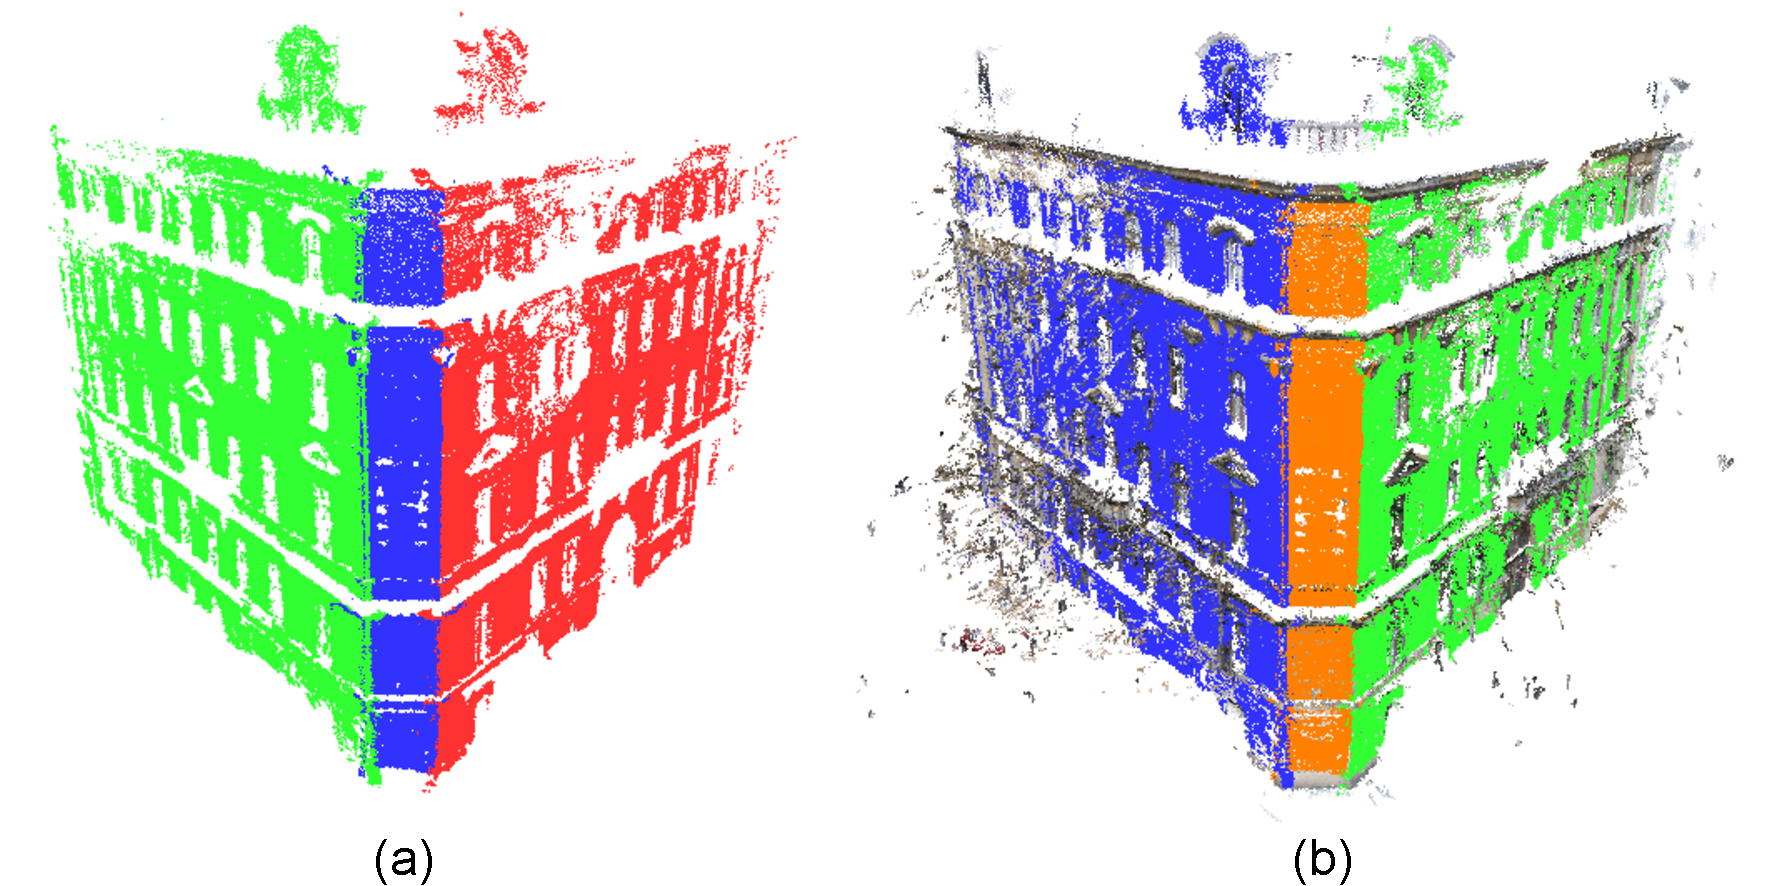
\includegraphics[width=\textwidth]{figures/test-d2}
\caption{Segmentace mračna dům 2. (a) zobrazuje pouze segmentované body, (b) zobrazuje kromě segmentů i body, které nebyly segmentovány.}
\label{fig:test-d2}
\end{center}
\end{figure}

Výsledek segmentace považuji za správný a bez větších problémů. Bylo segmentováno 67\% ze všech bodů, zde by byl možná ještě prostor pro zlepšení, pravděpodobně by bylo možné přidat ještě cca 5\% bodů, které do segmentů patří. Zbylé body jsou však jen šum a do žádných rovin nepatří, jak je vidět na obrázku \ref{fig:test-d2} (b). 

%\newpage
\cleardoublepage
\subsubsection{Stodůlky}

Vstupní mračno je zobrazeno na obrázku \ref{fig:dum-stodulky}. Segmentace byla v tomto případě provedena ve dvou krocích, nejprve bylo mračno segmentováno s parametrem klastrování 9, poté bylo provedeno klastrování ve zbylém akumulátorovém poli s parametrem 12. Výsledky segmentace jsou uvedeny v tabulce \ref{table:test-st}, ukázka segmentovaných dat je na obrázku \ref{fig:test-st}.

\begin{table}[ht]
\resizebox{\textwidth}{!} {
\begin{tabular}{|l|c|l|l|r|r|r|r|r|r|c|}
\hline
\textbf{} & \multicolumn{ 3}{c|}{\textbf{Parametry}} & \multicolumn{ 3}{c|}{\textbf{Body}} & \multicolumn{ 3}{c|}{\textbf{Segmenty}} &\ldots\\ \hline
\multicolumn{1}{|c|}{\textbf{test}} & \textbf{P1} & \multicolumn{1}{c|}{\textbf{P2}} & \multicolumn{1}{c|}{\textbf{P3}} & \multicolumn{1}{c|}{\textbf{Celkem}} & \multicolumn{ 2}{c|}{\textbf{Segmentováno}} & \multicolumn{1}{c|}{\textbf{Nalezeno}} & \multicolumn{1}{c|}{\textbf{Očekáváno }} & \multicolumn{1}{c|}{\textbf{Správných}} &\ldots\\ \hline
st-1.0 & \multicolumn{1}{r|}{48} & \multicolumn{1}{r|}{9} & \multicolumn{1}{r|}{10} & 604411 & 406188 & 67,20\% & 14 & 21 & 12 &\ldots\\ \hline
st-1.1 & \multicolumn{1}{r|}{48} & \multicolumn{1}{r|}{12} & \multicolumn{1}{r|}{10} & 604411 & 16408 & 2,71\% & 3 & 7 & 3 &\ldots\\ \hline
celkem: & \multicolumn{1}{l|}{} &  &  & 604411 & 422596 & 69,92\% & 17 & 21 & 15&\ldots \\ \hline
\end{tabular}
}
\begin{flushright} \scalebox{0.9} {
\begin{tabular}{|c|r|r|r|r|r|}
\hline
\ldots& \multicolumn{ 5}{|c|}{\textbf{Čas [s]}} \\ \hline
\ldots& \multicolumn{1}{|c|}{\textbf{Celkem}} & \multicolumn{1}{c|}{\textbf{Segmentace}} & \multicolumn{1}{c|}{\textbf{Klastrování}} & \multicolumn{1}{c|}{\textbf{Kd-strom}} & \multicolumn{1}{c|}{\textbf{SVD}} \\ \hline
\ldots& 190,39 & 118,19 & 72,21 & 34,62 & 36,47 \\ \hline
\ldots& 15,07 & 0 & 15,07 & 0 & 0,02 \\ \hline
\ldots& 205,46 & 118,19 & 87,27 & 34,62 & 36,49 \\ \hline
\end{tabular}
}\end{flushright}

\caption{Tabulka zobrazuje informace o segmentaci mračna stodůlky. Parametry jsou popsány v příloze \ref{chap:zkratky}.} 
\label{table:test-st}
\end{table}

\begin{figure}[H]
\begin{center}
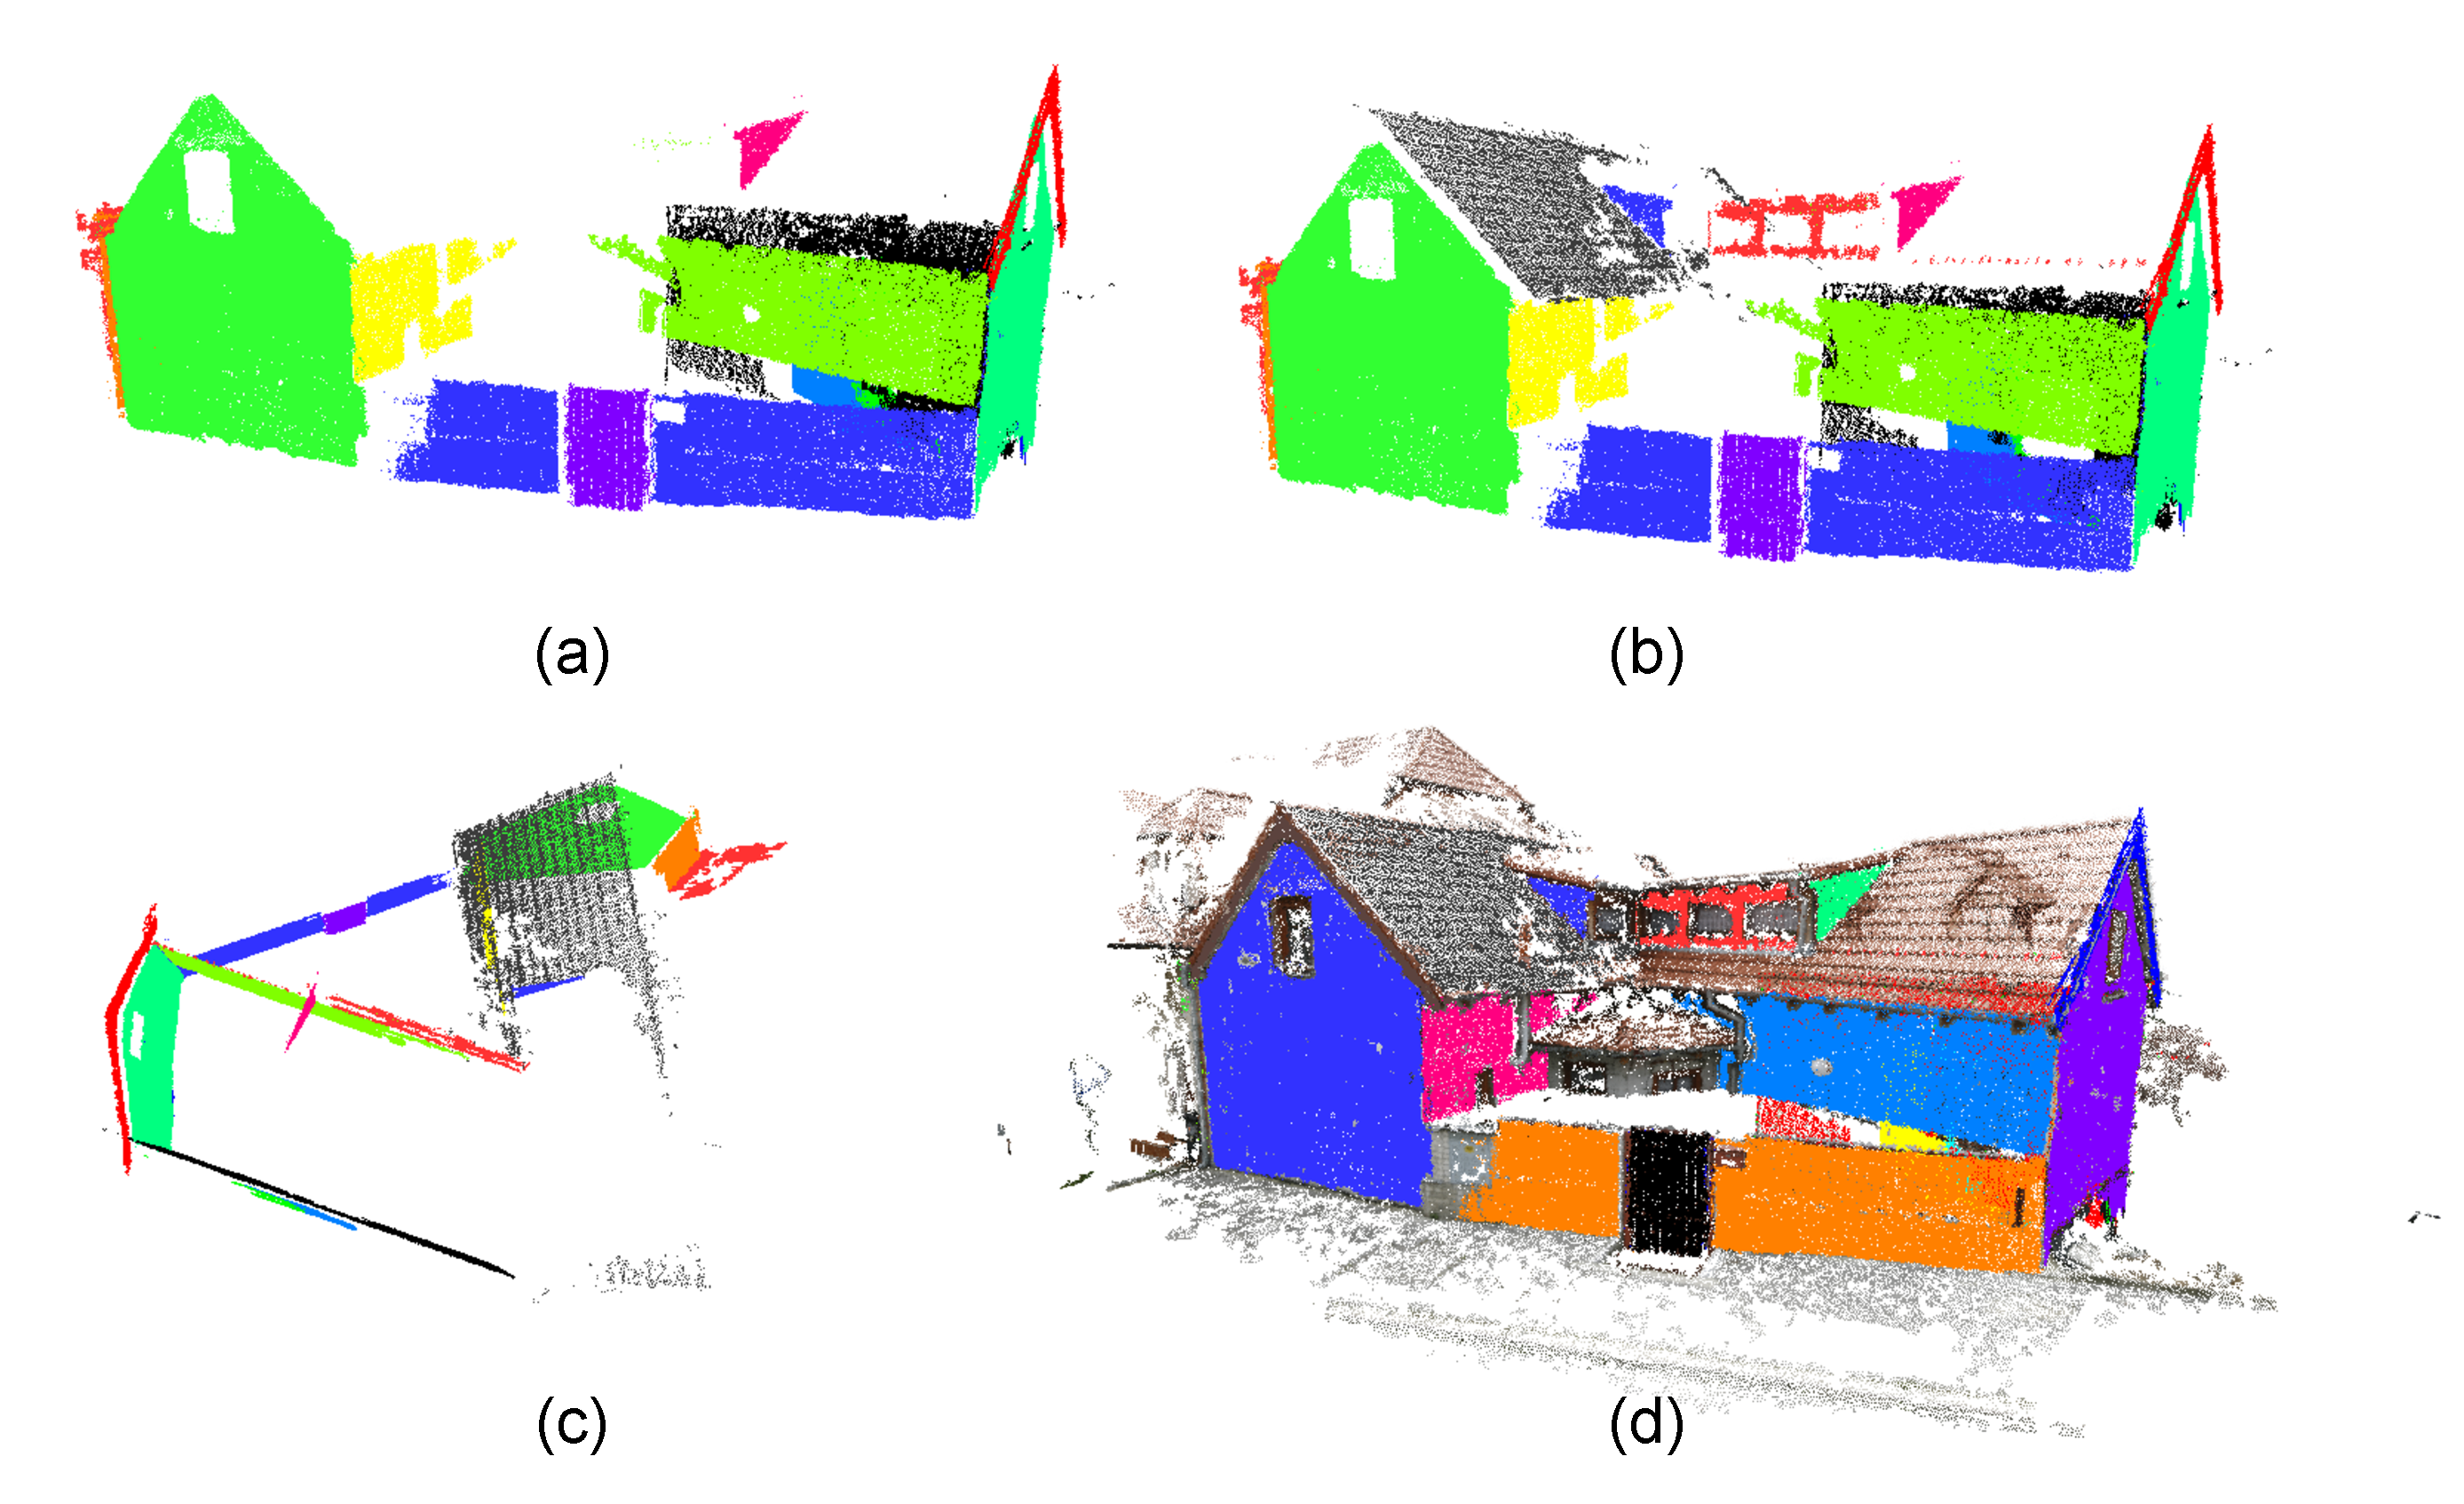
\includegraphics[width=\textwidth]{figures/test-st}
\caption{Segmentace mračna stodůlky. (a) zobrazuje první část segmentace, (b) zobrazuje celkovou segmentaci, (c) zobrazuje pohled na celkovou segmentaci shora, (d) zobrazuje celkovou segmentaci včetně bodů, které nebyly segmentovány.}
\label{fig:test-st}
\end{center}
\end{figure}

\begin{changeheight}{3cm}
Tato segmentace již není tak bezproblémová, jako ta předchozí. Na první pohled je patrné, že střecha na pravé části domu nebyla rozeznána. To je způsobeno tím, že povrch střechy je hrbolatý a proto není výpočet parametrů příliš přesný. Navíc střecha obsahuje menší počet bodů, než by se na první pohled zdálo (body jsou zde řidší, než na stěnách). Z těchto dvou důvodů body ze střechy nevytvoří v akumulátorovém poli dostatečný vrchol, aby byl segment rozeznán. V tomto případě nepomůže ani výrazně zvětšení parametru definujícího okolí. Dále jsem uvedl 21 očekávaných segmentů a nalezených pouze 15. Nebylo tedy nalezeno ještě 5 dalších segmentů - nicméně tyto plochy jsou již velmi malé a algoritmus je v zašuměném akumulátorovém poli nenašel. Dále byly nalezeny 2 segmenty, které jsem neoznačil jako správné. Tyto segmenty byly vytvořeny ze \uv{zbytků} jiného segmentu při iterativním prohledávání pole - vznikla tedy situace, kdy jsou nalezeny 2 segmenty v jedné rovině - tento problém byl již popsán dříve, v sekci \ref{sub:vliv-param}. Jeden z těchto segmentů je na zadní straně mračna (zelená a modrá stěna), druhý chybný segment je příliš malý, aby byl na obrázku zřetelný. 

V tomto případě je za nenalezené segmenty zodpovědné větší množství šumu a duplicita v datech. Šum nedovoluje prohledávat akumulátorové pole příliš podrobně a mračno navíc obsahuje velké množství duplicitních bodů (obě čelní stěny jsou v mračnu dvakrát). To zbytečně zvyšuje velikost akumulátorového pole, tím pádem nejsou vrcholy v poli tak výrazné. Mračno stodůlky je rozděleno do tří souborů. Jeden z těchto souborů obsahuje polovinu bodů, ale naprostou většinu rovin. Navíc neobsahuje duplicitní body (jednotlivé soubory se překrývají, tím vznikají duplicity). Pokud provedu segmentaci pouze na tomto jednom souboru, výsledky jsou výrazně lepší, viz tabulka \ref{table:test-st-2} a obrázek \ref{fig:test-st-2}. 

\begin{table}[ht]
\resizebox{\textwidth}{!} {
\begin{tabular}{|r|r|r|r|r|r|r|r|r|r|r|}
\hline
&\multicolumn{3}{c|}{\textbf{Parametry}} & \multicolumn{3}{c|}{\textbf{Body}} & \multicolumn{3}{c|}{\textbf{Segmenty}}&\ldots\\ \hline
\textbf{test} & \textbf{P1} & \textbf{P2} & \textbf{P3} & \textbf{Celkem} & \multicolumn{2}{c|}{\textbf{Segmentováno}} & \textbf{Nalezeno} & \textbf{Očekáváno} & \textbf{Správných} &\ldots\\ \hline
st-2.0 & 70 & 12 & 2 & 291232 & 215678 & 74,06\% & 18 & 19 & 18 &\ldots\\ \hline
\end{tabular}
}\\ \\
\begin{flushright} \scalebox{0.9} {
\begin{tabular}{|l|r|r|r|r|r|}
\hline
\ldots&\multicolumn{5}{|c|}{\textbf{Čas [s]}} \\ \hline
\ldots&\textbf{Celkem} & \textbf{Segmentace} & \textbf{Klastrování} & \textbf{kd-strom} & \textbf{SVD} \\\hline
\ldots&80,45 & 69,42 & 11,03 & 19,22 & 22,49 \\ \hline
\end{tabular}
}\end{flushright}

\caption{Tabulka zobrazuje informace o segmentaci části mračna stodůlky.} 
\label{table:test-st-2}
\end{table}

\begin{figure}[H]
\begin{center}
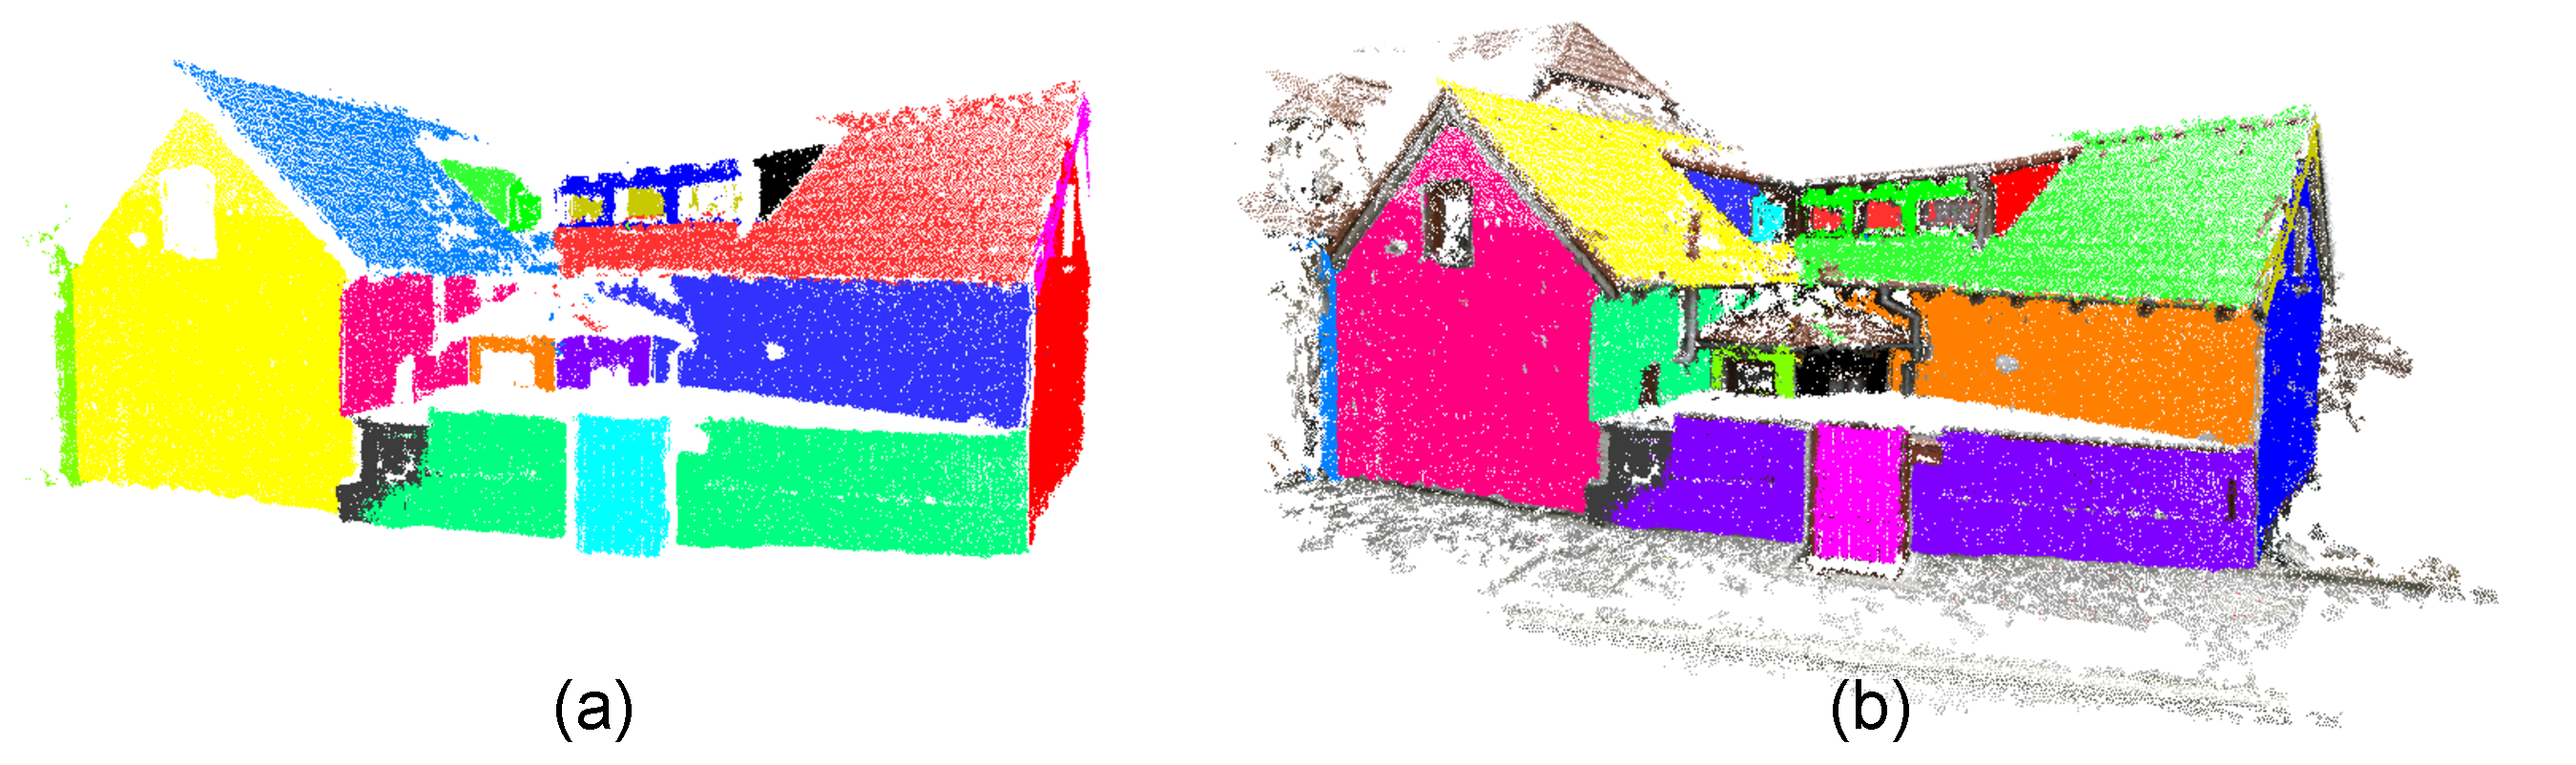
\includegraphics[width=\textwidth]{figures/test-st-2}
\caption{Segmentace mračna stodůlky. (a) zobrazuje pouze segmentaci, (b) zobrazuje segmentaci včetně bodů, které nebyly segmentovány.}
\label{fig:test-st-2}
\end{center}
\end{figure}
V tomto případě byly nalezeny správně všechny rovinné segmenty kromě malé střechy vlevo nahoře, která obsahuje jen velmi málo bodů a není příliš rovná. Z testu vyplývá, že algoritmus je citlivý na různou hustotu bodů v rámci jednotlivých rovin (způsobenou duplicitami v původním mračnu), a že šum v datech může zhoršit výsledky segmentace.
\end{changeheight}


\cleardoublepage
\subsubsection{Červená Lhota}

Toto mračno reprezentuje zámek Červená Lhota. Mračno obsahuje poměrně velké množství bodů, které jsou velmi daleko od snímaného objektu (šum) a výrazná část bodů je obsažena mimo stěny budovy, viz obrázek \ref{fig:cervena-lhota}. Mračno je tedy poměrně odlišné od dvou předchozích a bude zajímavé, jak si s ním algoritmus poradí.

\begin{figure}[H]
\begin{center}
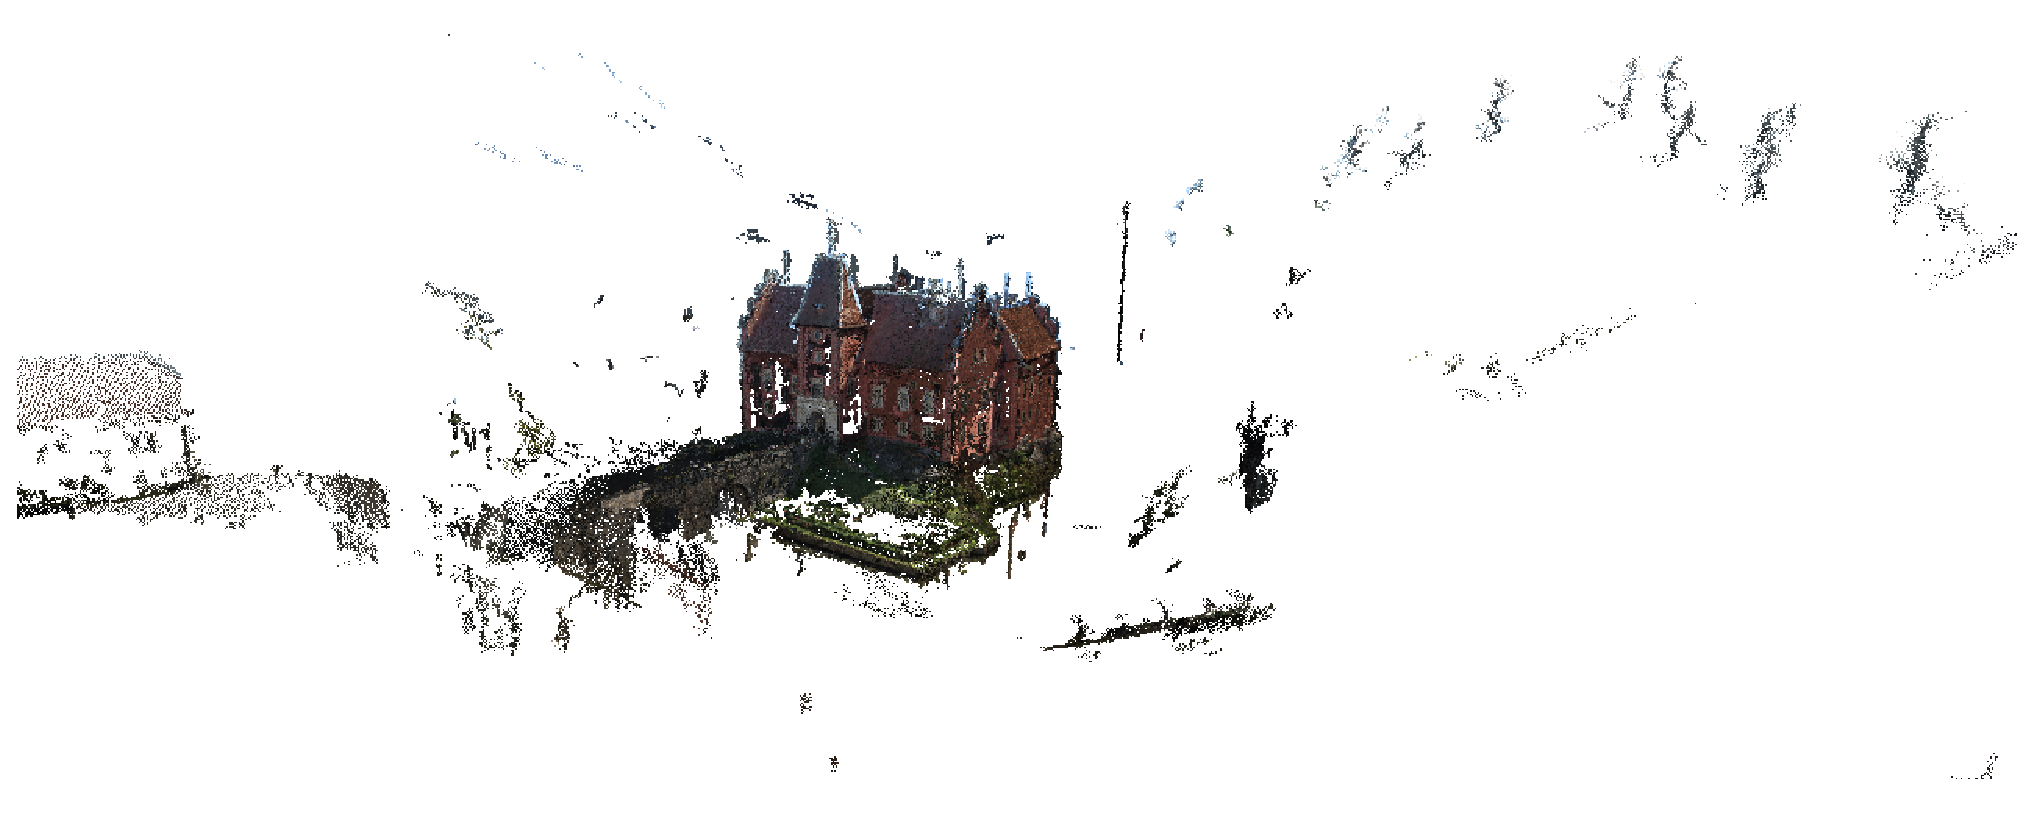
\includegraphics[width=\textwidth]{figures/cervena-lhota}
\caption{Ukázka mračna Červená Lhota.}
\label{fig:cervena-lhota}
\end{center}
\end{figure}

Výsledky segmentace jsou zaznamenány v tabulce \ref{table:test-cl} a ukázka výsledné segmentace z různých úhlů je vidět na obrázku \ref{fig:test-cl}. Obrázky této segmentace bohužel nejsou tolik přehledné jako u předešlých testování, lepší je prohlédnou si celé mračno na přiloženém CD.

\begin{table}[ht]
\resizebox{\textwidth}{!} {
\begin{tabular}{|r|r|r|r|r|r|r|r|r|r|r|}
\hline
\textbf{} & \multicolumn{ 3}{c|}{\textbf{Parametry}} & \multicolumn{ 3}{c|}{\textbf{Body}} & \multicolumn{ 3}{c|}{\textbf{Segmenty}}&\ldots \\ \hline
\multicolumn{1}{|c|}{\textbf{test}} & \textbf{P1} & \multicolumn{1}{c|}{\textbf{P2}} & \multicolumn{1}{c|}{\textbf{P3}} & \textbf{Celkem} & \multicolumn{ 2}{c|}{\textbf{Segmentováno}} & \textbf{Nalezeno} & \multicolumn{1}{c|}{\textbf{Očekáváno }} & \multicolumn{1}{c|}{\textbf{Správných}}&\ldots \\ \hline
cl-0.0 & \multicolumn{1}{r|}{60} & \multicolumn{1}{r|}{10} & \multicolumn{1}{r|}{5} & \multicolumn{1}{r|}{611095} & \multicolumn{1}{r|}{331336} & \multicolumn{1}{r|}{54,22\%} & \multicolumn{1}{r|}{16} & \multicolumn{1}{r|}{18} & \multicolumn{1}{r|}{16} &\ldots\\ \hline
\end{tabular}
}
\begin{flushright} \scalebox{0.9} {
\begin{tabular}{|r|r|r|r|r|r|}
\hline
\ldots & \multicolumn{ 5}{|c|}{\textbf{Čas [s]}} \\ \hline
\ldots &\textbf{Celkem} & \multicolumn{1}{c|}{\textbf{Segmentace}} & \multicolumn{1}{c|}{\textbf{Klastrování}} & \multicolumn{1}{c|}{\textbf{kd-strom}} & \multicolumn{1}{c|}{\textbf{SVD}} \\ \hline
\ldots &\multicolumn{1}{|r|}{328,81} & \multicolumn{1}{r|}{163,63} & \multicolumn{1}{r|}{165,18} & \multicolumn{1}{r|}{48,19} & \multicolumn{1}{r|}{50,83} \\ \hline
\end{tabular}
}\end{flushright}

\caption{Tabulka zobrazuje informace o segmentaci mračna bodů Červená Lhota. Parametry jsou popsány v příloze \ref{chap:zkratky}.} 
\label{table:test-cl}
\end{table}

\begin{figure}[ht]
\begin{center}
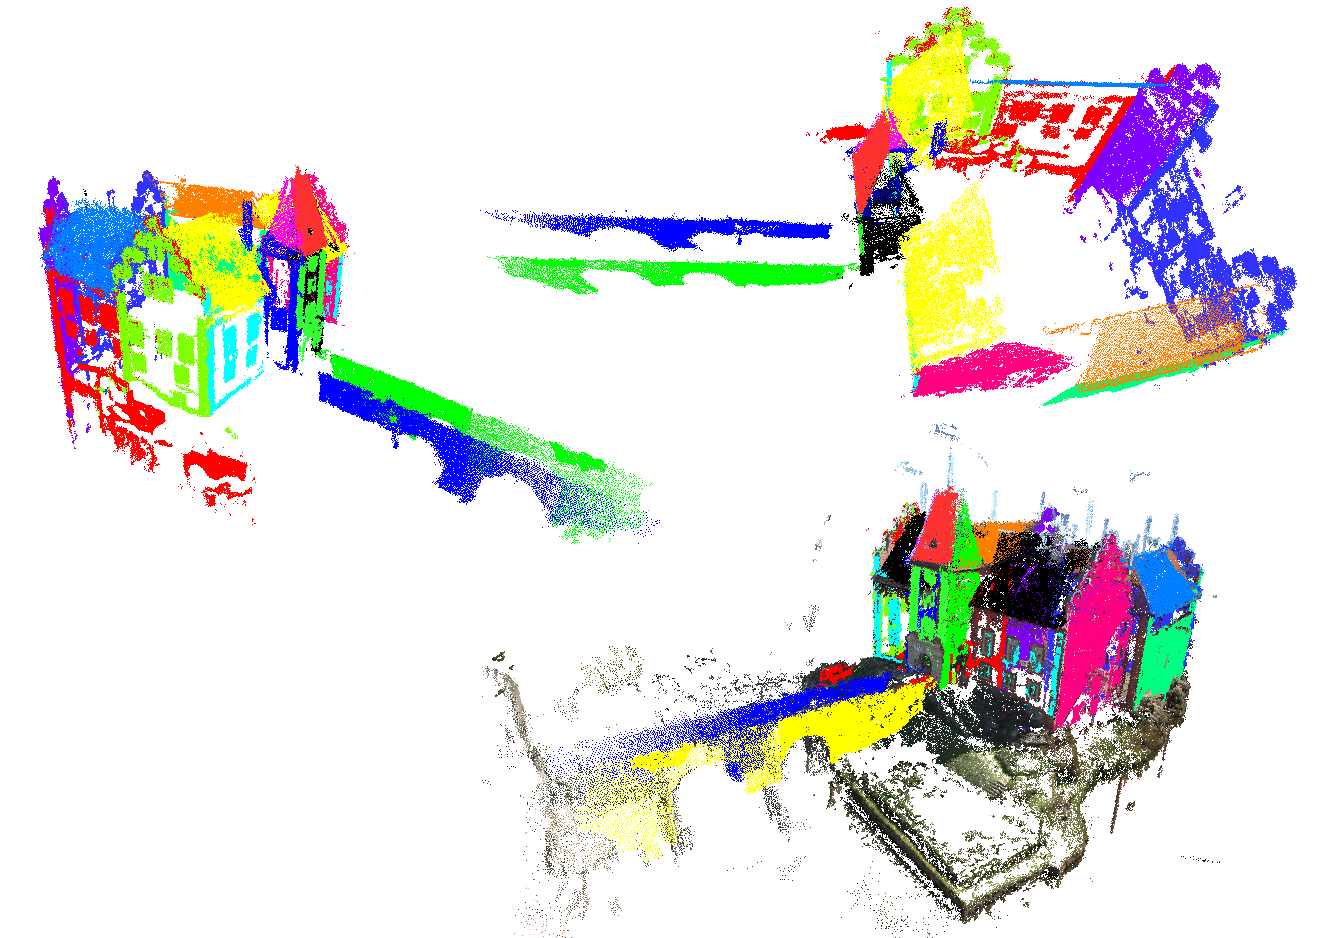
\includegraphics[width=\textwidth]{figures/test-cl}
\caption{Ukázka segmentace mračna Červená Lhota z různých úhlů.}
\label{fig:test-cl}
\end{center}
\end{figure}

Segmentace identifikovala téměř všechny roviny v rámci hlavního objektu. V tabulce je uvedeno, že nebyly nalezeny 2 roviny. Algoritmus nenašel střechu na zadní straně. Střechu našel při zvýšení parametru klastrování, ale to se již také začaly objevovat chybné segmenty, proto jsem vybral na ukázku tuto segmentaci, i když tuto jednu rovinu nenalezla. Poté ještě nebyla malá rovina spojující boční stěny na pravé straně zámku, ta obsahuje poměrně málo bodů, pravděpodobně proto již nebyla při segmentaci rozpoznána.

Dále by se mohlo zdát, že z čelní a levé strany chybí v segmentech body. To ale není chyba algoritmu, v těchto stěnách je takto málo bodů už ve vstupním mračnu, algoritmus jich naopak segmentoval naprostou většinu. Výraznější chyba v segmentaci je červená rovina vlevo, která zahrnuje i body, které již nepatří do stěny, ale jde o část skály. Rovina měla pravděpodobně již od začátku větší RMS, proto se takto \uv{rozrostla} i o body, které do ní přímo nepatří, včetně několika bodů ze sousedních stěn. Takovéto chybě se nedá jednoduše vyhnout, pokud je již ze začátku kvalita roviny (velikost RMS) horší, rovina často obsáhne i okolní body, které do ní již přímo nespadají.

Celkově bych však segmentaci ohodnotil jako úspěšnou, kromě dvou menších rovin byly na objektu rozeznány všechny stěny. Segmenty navíc obsahují naprostou většinu bodů z těchto rovin. Segmentace také nebyla viditelně ovlivněna větším množstvím chybných bodů mimo roviny.

\cleardoublepage
\subsubsection{Doudleby}

Toto mračno reprezentuje zámek Doudleby nad Orlicí. Mračno je poměrně velké a obsahuje několik výrazných rovin, viz obrázek \ref{fig:doudleby}.

\begin{figure}[H]
\begin{center}
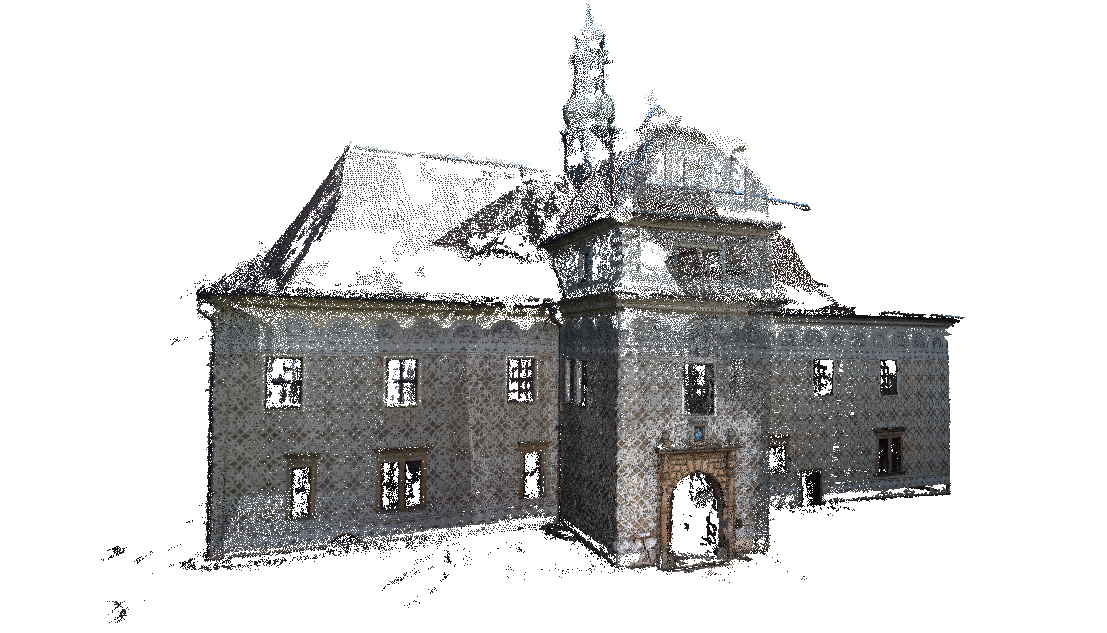
\includegraphics[width=\textwidth]{figures/doudleby}
\caption{Ukázka mračna Doudleby.}
\label{fig:doudleby}
\end{center}
\end{figure}

Výsledky segmentace jsou zaznamenány v tabulce \ref{table:test-do} a ukázka výsledné segmentace z různých úhlů je vidět na obrázku \ref{fig:test-do}.

\begin{table}[ht]
\resizebox{\textwidth}{!} {
\begin{tabular}{|r|r|r|r|r|r|r|r|r|r|c|}
\hline
\textbf{} & \multicolumn{ 3}{c|}{\textbf{Parametry}} & \multicolumn{ 3}{c|}{\textbf{Body}} & \multicolumn{ 3}{c|}{\textbf{Segmenty}} &\ldots\\ \hline
\multicolumn{1}{|c|}{\textbf{test}} & \textbf{P1} & \multicolumn{1}{c|}{\textbf{P2}} & \multicolumn{1}{c|}{\textbf{P3}} & \textbf{Celkem} & \multicolumn{ 2}{c|}{\textbf{Segmentováno}} & \textbf{Nalezeno} & \multicolumn{1}{c|}{\textbf{Očekáváno }} & \multicolumn{1}{c|}{\textbf{Správných}} &\ldots\\ \hline
do-0.0 & \multicolumn{1}{r|}{80} & \multicolumn{1}{r|}{20} & \multicolumn{1}{r|}{10} & \multicolumn{1}{r|}{1299900} & \multicolumn{1}{r|}{1032386} & \multicolumn{1}{r|}{79,42\%} & \multicolumn{1}{r|}{11} & \multicolumn{1}{r|}{16} & \multicolumn{1}{r|}{11} &\ldots\\ \hline
\end{tabular}
}
\begin{flushright} \scalebox{0.9} {
\begin{tabular}{|c|r|r|r|r|r|}
\hline
\ldots& \multicolumn{ 5}{|c|}{\textbf{Čas [s]}} \\ \hline
\ldots& \textbf{Celkem} & \multicolumn{1}{c|}{\textbf{Segmentace}} & \multicolumn{1}{c|}{\textbf{Klastrování}} & \multicolumn{1}{c|}{\textbf{Kd-strom}} & \multicolumn{1}{c|}{\textbf{SVD}} \\ \hline
\ldots& \multicolumn{1}{|r|}{660,43} & \multicolumn{1}{r|}{542,61} & \multicolumn{1}{r|}{117,82} & \multicolumn{1}{r|}{149,93} & \multicolumn{1}{r|}{174,69} \\ \hline
\end{tabular}
}\end{flushright}

\caption{Tabulka zobrazuje informace o segmentaci mračna bodů Doudleby. Parametry jsou popsány v příloze \ref{chap:zkratky}.} 
\label{table:test-do}
\end{table}

\begin{figure}[ht]
\begin{center}
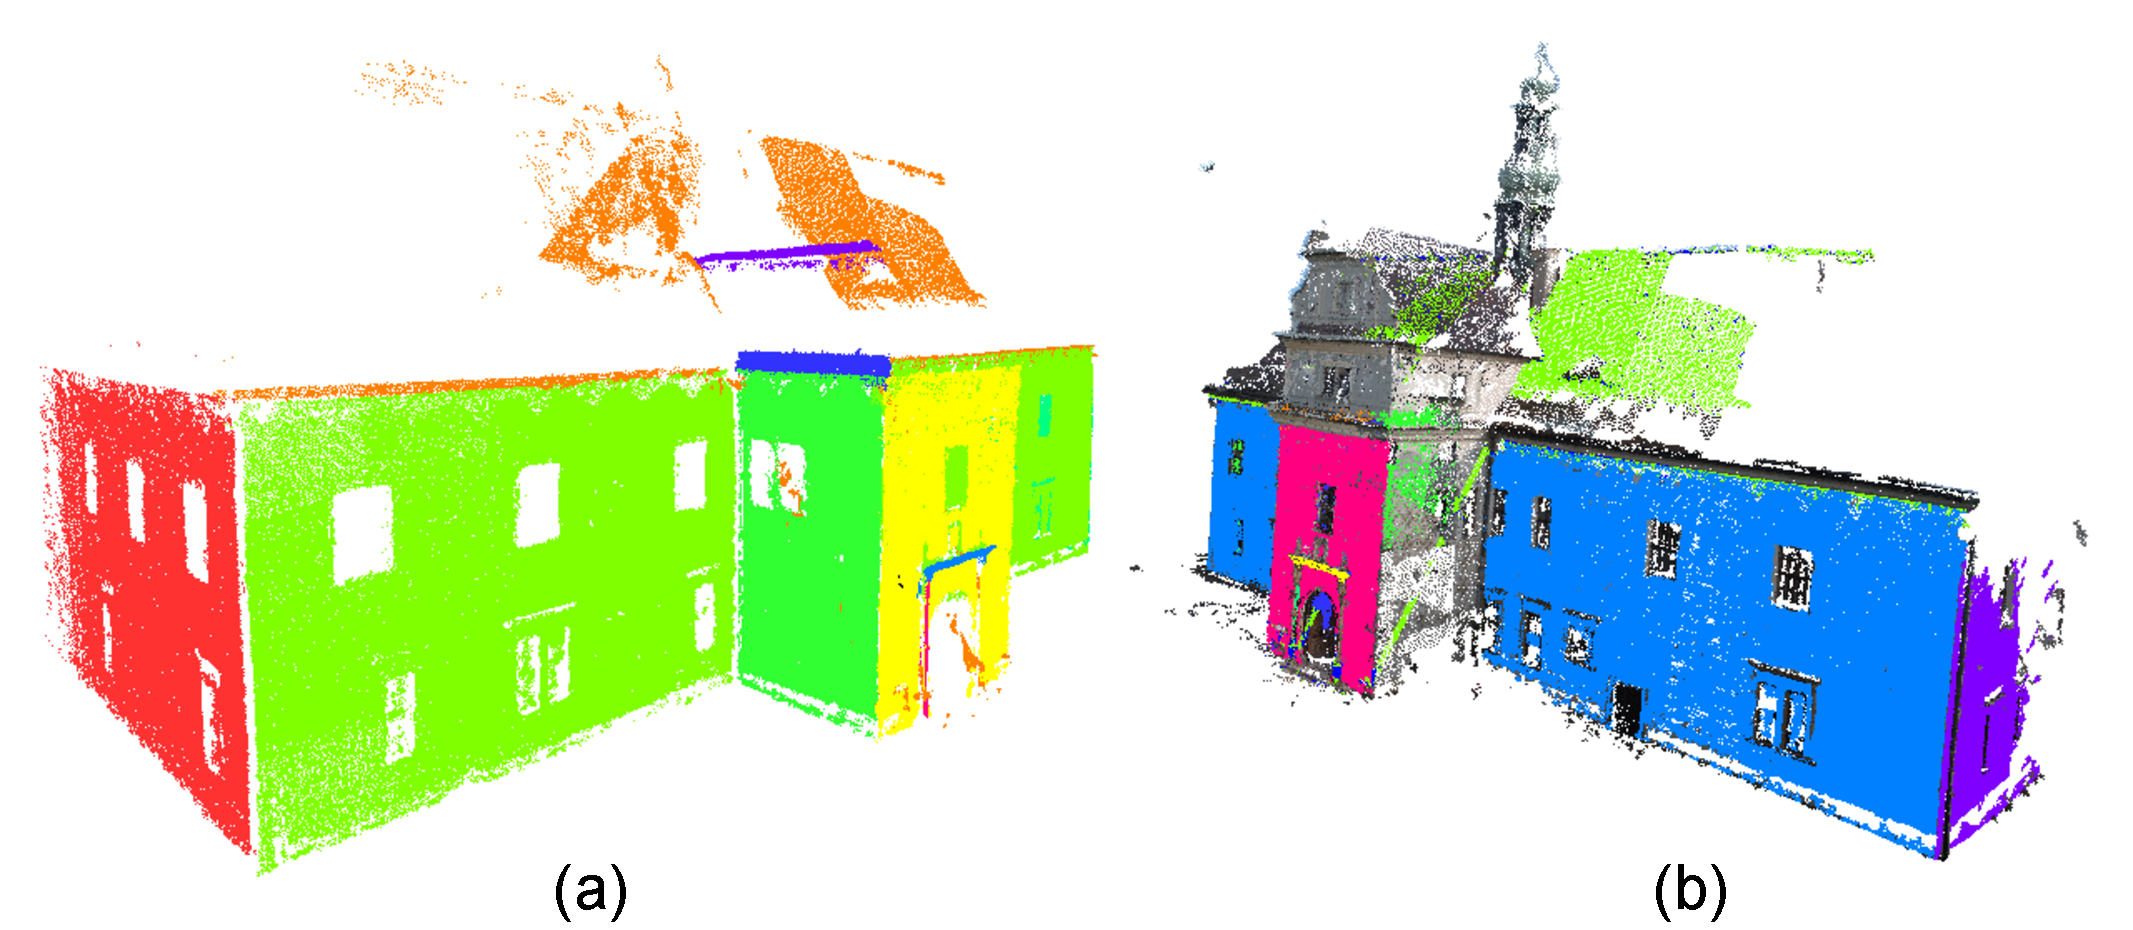
\includegraphics[width=\textwidth]{figures/test-do}
\caption{Ukázka segmentace mračna Doudleby. (a) zobrazuje pouze nalezené segmenty, (b) zobrazuje segmenty včetně bodů, které nebyly segmentovány.}
\label{fig:test-do}
\end{center}
\end{figure}

Segmentace mračna sice segmentovala téměř 80\% bodů, nicméně nenalezla 5 rovin. Nebyla nalezena levá část střechy, dále chybí celá pravá část vstupní části budovy. Dále nebyly nalezeny 3 menší segmenty zepředu a na boku vstupní části budovy. Všechny tyto segmenty mají společnou jednu vlastnost, a to je velmi malá hustota bodů oproti ostatním stěnám. Domnívám se, že kvůli této malé hustotě bodů není výpočet parametrů tak přesný, navíc celkově obsahují tyto nenalezené roviny malý počet bodů. K tomu se ještě přidává fakt, že celkově toto mračno obsahuje téměř 1,3 milionu bodů, takže vytvořené akumulátorové pole je poměrně velké. Myslím si, že spojení těchto tří vlivů dohromady způsobilo nenalezení těchto menších segmentů. Myslím si ale, že je to spíše problém celé této metody segmentace, než konkrétní implementace. Segmentace je založena zejména na tom, že roviny vytvoří vrchol v akumulátorovém poli. Pokud však několik různých vlivů způsobí, že body v rovině nevytvoří výrazný vrchol, není téměř možné toto detekovat a tím pádem ani řešit.

Aby byla nalezena aspoň ta největší střecha, bylo nutné použít větší parametr pro velikost okolí (80), což v kombinaci s téměř 1,3 miliony body způsobilo, že segmentace trvala 11 minut. To je výrazně více, než u všech předešlých testů. Celkově však segmentace není úplně špatná. U rovin, které byly nalezeny, byly segmentovány téměř všechny možné body a celkově bylo segmentováno téměř 80\% ze všech vstupních bodů. 


\cleardoublepage
\subsubsection{Faustův dům}

Vstupní mračno zachycuje část Faustova domu na Karlově náměstí. Mračno je zobrazeno na obrázku \ref{fig:faust}. Toto mračno je největší, které jsem měl při testování k dispozici, obsahuje necelých 1,5 milionu bodů.

\begin{figure}[H]
\begin{center}
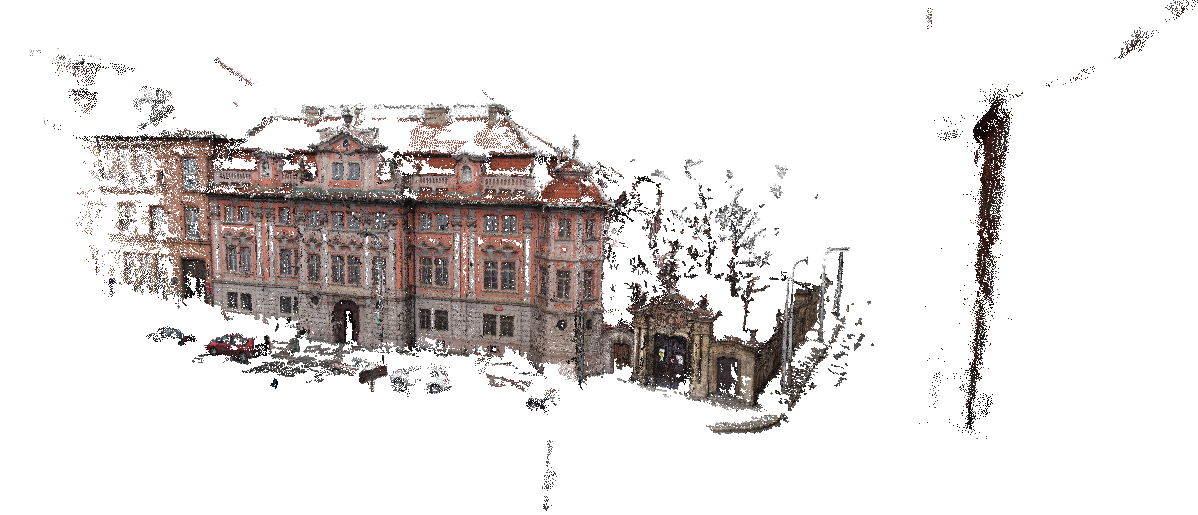
\includegraphics[width=\textwidth]{figures/faust}
\caption{Ukázka mračna Faust.}
\label{fig:faust}
\end{center}
\end{figure}

Výsledky testování jsou uvedeny v tabulce \ref{table:test-fa} a ukázka segmentace je zobrazena na obrázku \ref{fig:test-fa}.

\begin{table}[ht]
\resizebox{\textwidth}{!} {
\begin{tabular}{|l|r|r|r|r|r|r|r|r|r|c|}
\hline
\textbf{} & \multicolumn{ 3}{c|}{\textbf{Parametry}} & \multicolumn{ 3}{c|}{\textbf{Body}} & \multicolumn{ 3}{c|}{\textbf{Segmenty}} &\ldots \\ \hline
\multicolumn{1}{|c|}{\textbf{test}} & \textbf{P1} & \multicolumn{1}{c|}{\textbf{P2}} & \multicolumn{1}{c|}{\textbf{P3}} & \textbf{Celkem} & \multicolumn{ 2}{c|}{\textbf{Segmentováno}} & \textbf{Nalezeno} & \multicolumn{1}{c|}{\textbf{Očekáváno }} & \multicolumn{1}{c|}{\textbf{Správných}} &\ldots\\ \hline
fa-0.0 & \multicolumn{1}{r|}{35} & \multicolumn{1}{r|}{10} & \multicolumn{1}{r|}{10} & \multicolumn{1}{r|}{1492940} & \multicolumn{1}{r|}{965492} & \multicolumn{1}{r|}{64,67\%} & \multicolumn{1}{r|}{6} & \multicolumn{1}{r|}{8} & \multicolumn{1}{r|}{5} &\ldots\\ \hline
\end{tabular}

}
\begin{flushright} \scalebox{0.9} {
\begin{tabular}{|c|r|r|r|r|r|}
\hline
\ldots& \multicolumn{ 5}{|c|}{\textbf{Čas [s]}} \\ \hline
\ldots& \textbf{Celkem} & \multicolumn{1}{c|}{\textbf{Segmentace}} & \multicolumn{1}{c|}{\textbf{Klastrování}} & \multicolumn{1}{c|}{\textbf{Kd-strom}} & \multicolumn{1}{c|}{\textbf{SVD}} \\ \hline
\ldots& \multicolumn{1}{|r|}{1033,98} & \multicolumn{1}{r|}{336,76} & \multicolumn{1}{r|}{697,22} & \multicolumn{1}{r|}{93,58} & \multicolumn{1}{r|}{105,49} \\ \hline
\end{tabular}
}\end{flushright}

\caption{Tabulka zobrazuje informace o segmentaci mračna bodů Faustův dům. Parametry jsou popsány v příloze \ref{chap:zkratky}.} 
\label{table:test-fa}
\end{table}

\begin{figure}[ht]
\begin{center}
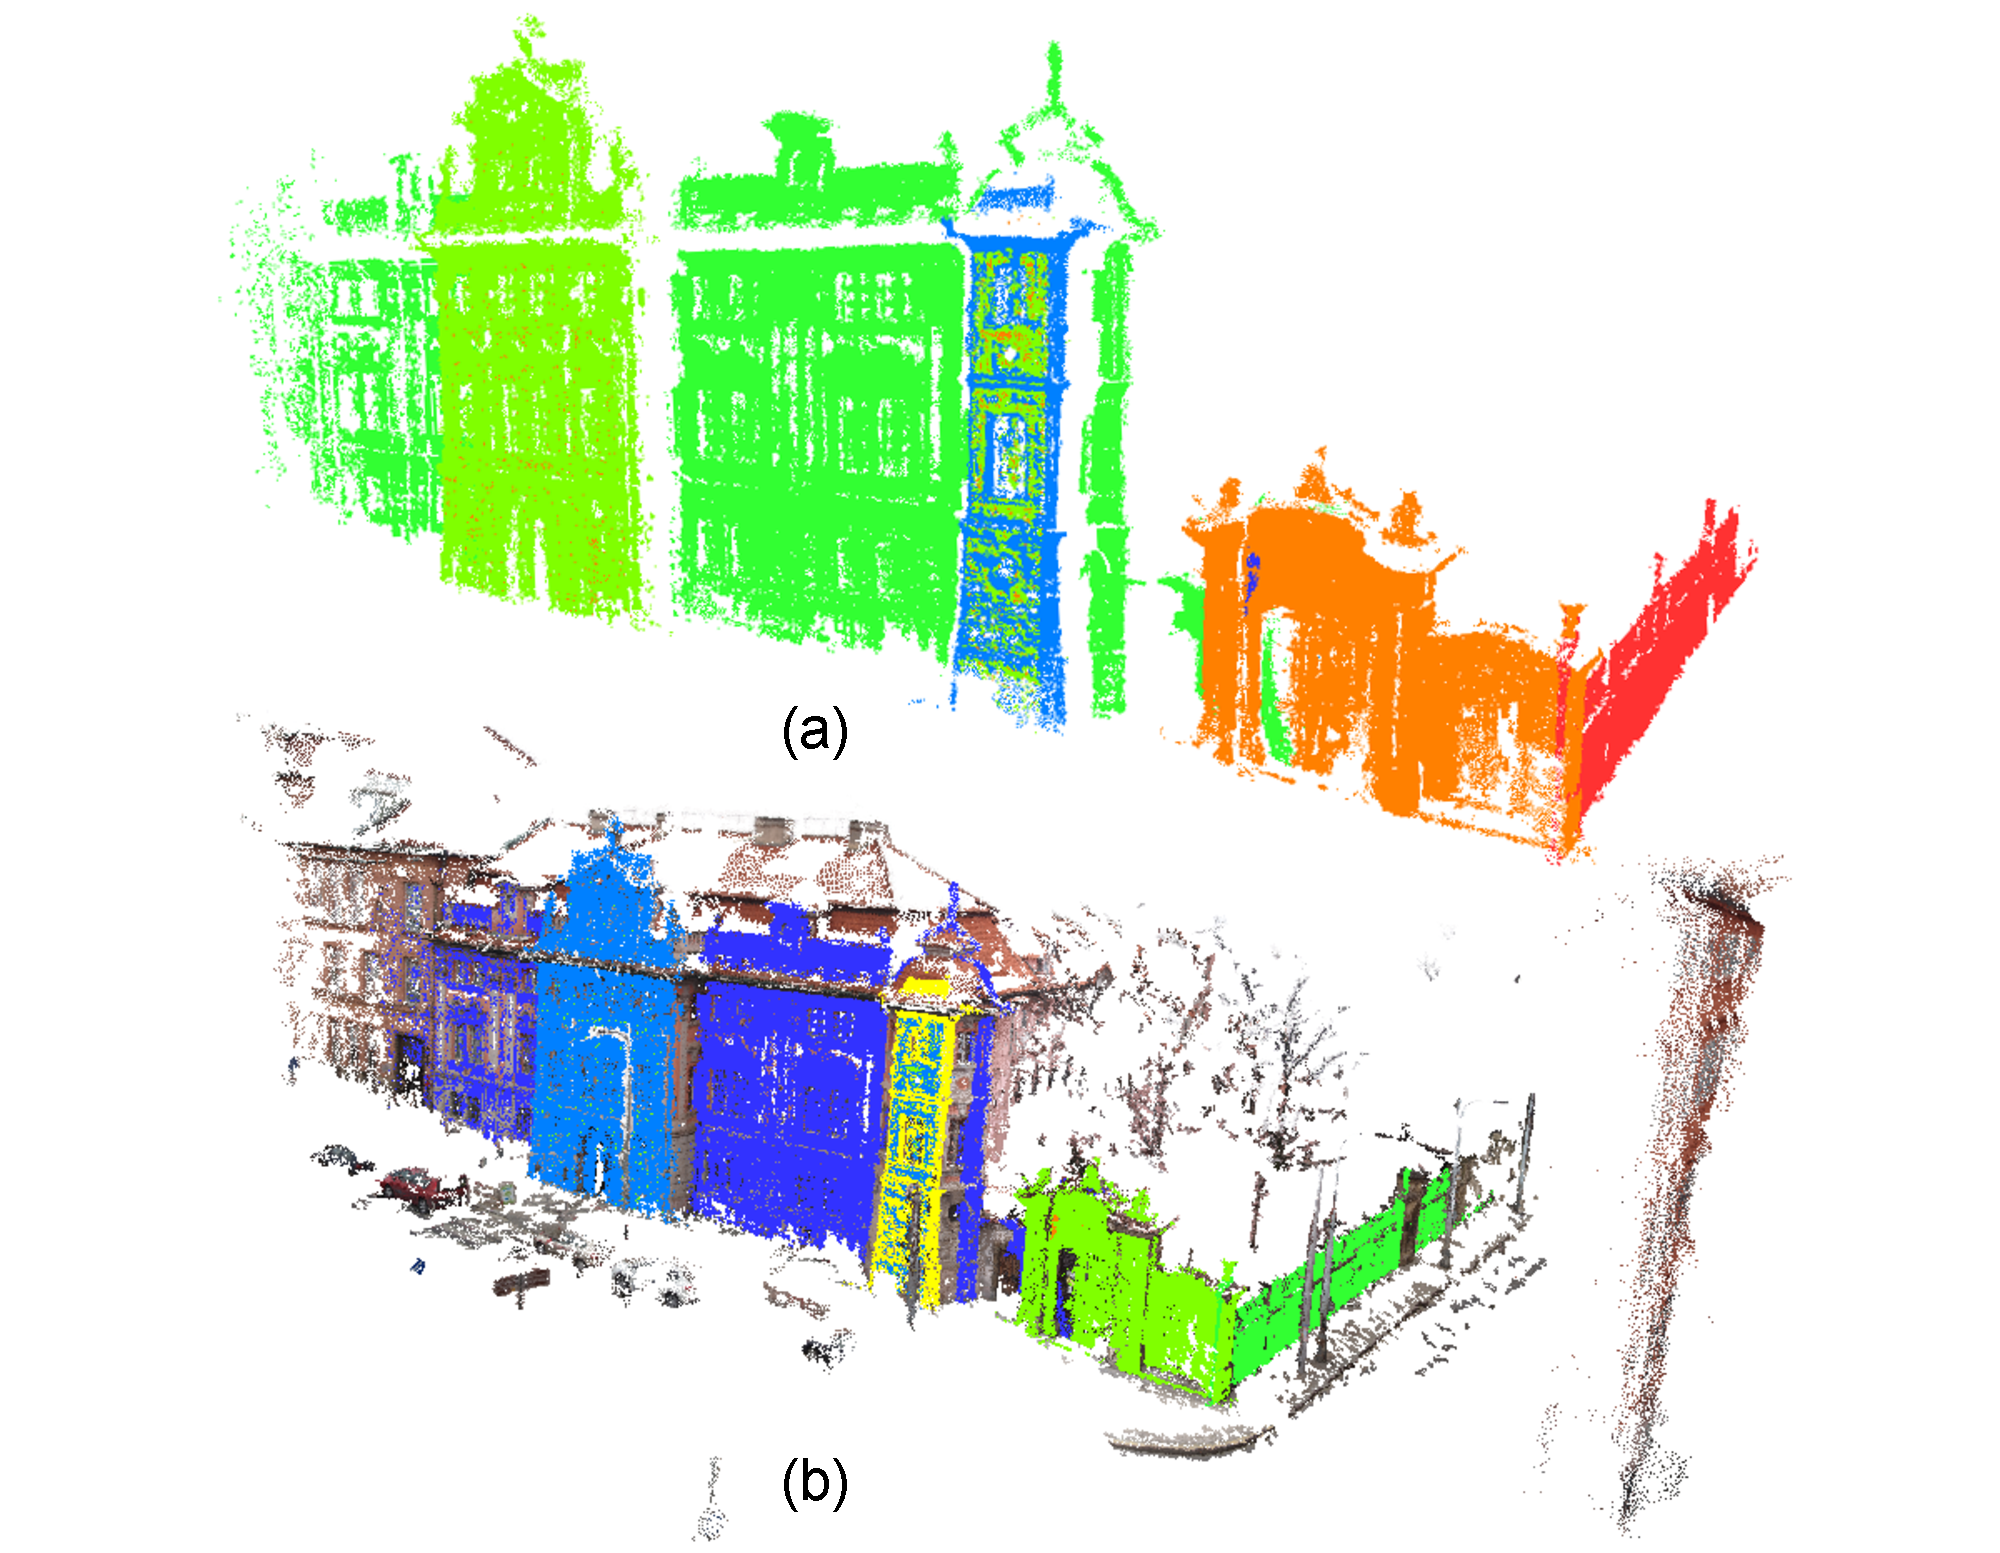
\includegraphics[width=\textwidth]{figures/test-fa}
\caption{Ukázka segmentace mračna Faustův dům. (a) zobrazuje pouze nalezené segmenty, (b) zobrazuje segmenty včetně bodů, které nebyly segmentovány.}
\label{fig:test-fa}
\end{center}
\end{figure}

Na této segmentaci se projevila chyba, kdy z jedné stěny nebyly vybrány všechny body a při další iteraci byl v té samé stěně nalezen nový segment. Tento problém byl již dříve v této kapitole popsán. Tomuto problému jsem se snažil vyhnout tím, že jsem nastavil kvalitu klastrování na 10. Doufal jsem, že při první iteraci bude vybrána většina bodů z roviny a v další iteraci již nezbydou body, které by byly rozeznány jako segment. Bohužel ani toto se neukázalo jako řešení, vedlejším důsledkem byl navíc velký čas klastrování bodů - více jak 11 minut, celkový čas segmentace přesáhl 17 minut a byl nejdelší ze všech testů.

Dále nebyly nalezeny menší roviny spojující největší stěny domu. Tyto roviny jsou ale velmi malé a zároveň rohy domu jsou při bližším pohledu výrazně zakulacené, takže pouze malá část z této roviny je doopravdy rovná. Bohužel je tato část příliš malá, aby jí algoritmus v tak velkém počtu bodů našel. Dále by se dalo segmentaci vytknout, že v levé části budovy mohlo být do segmentu přiřazeno více bodů.

Celkově bych tuto segmentaci označil za nejhorší ze všech testovaných. Všechny největší segmenty segmenty byly nalezeny, ale určitě je zde prostor pro zkvalitnění segmentace. 

\cleardoublepage
\subsubsection{Langweil}

Toto mračno je sken části Langweilova modelu Prahy, což je papírový model pražského starého města z devatenáctého století. Mračno je velmi malé, obsahuje pouze 125 tisíc bodů, mračno je zobrazeno na obrázku \ref{fig:langweil}

\begin{figure}[H]
\begin{center}
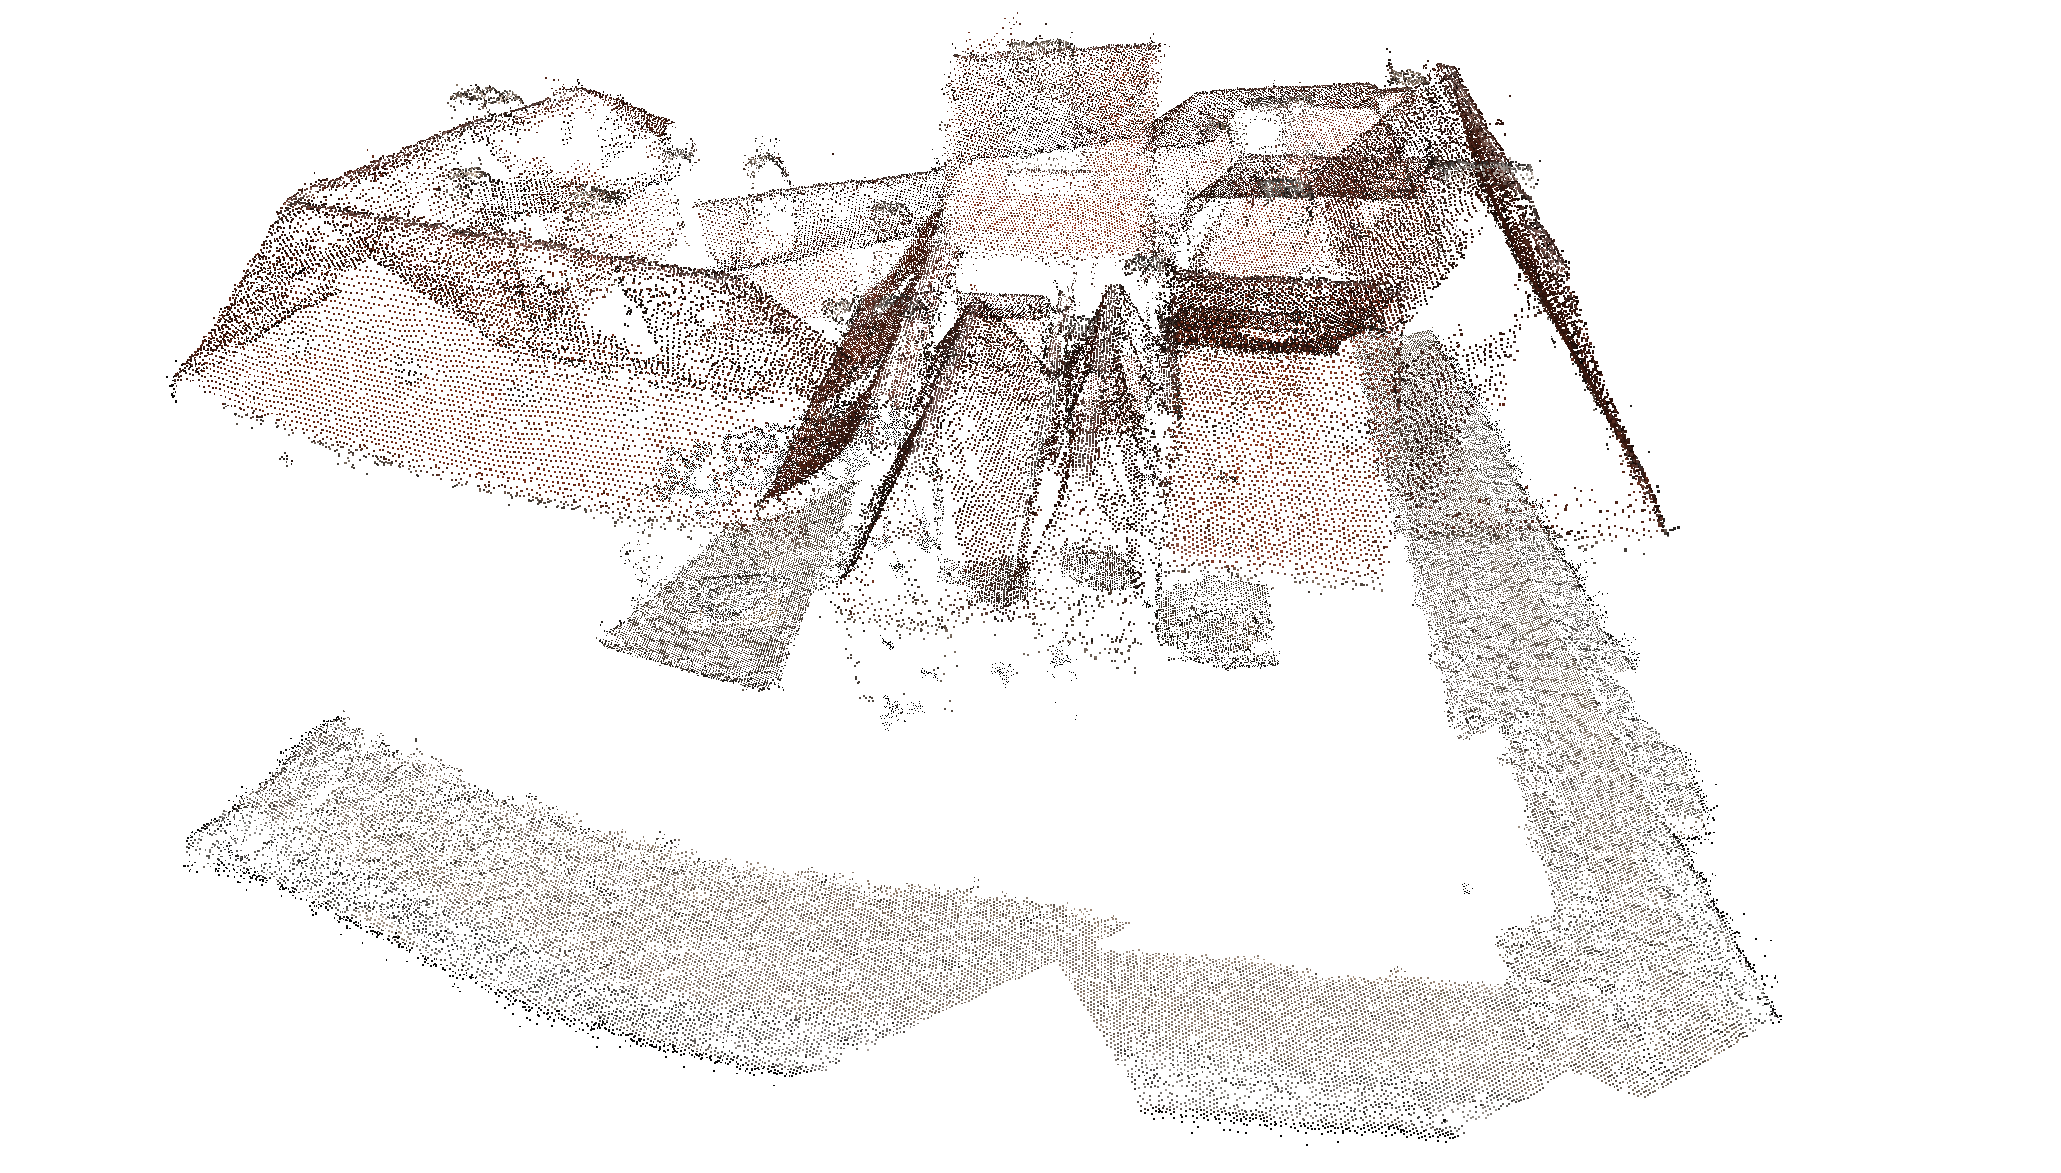
\includegraphics[width=\textwidth]{figures/langweil}
\caption{Ukázka mračna Langweil.}
\label{fig:langweil}
\end{center}
\end{figure}

Výsledky testování jsou uvedeny v tabulce \ref{table:test-lw} a ukázka segmentace je zobrazena na obrázku \ref{fig:test-lw}.

\begin{table}[ht]
\resizebox{\textwidth}{!} {
\begin{tabular}{|r|r|r|r|r|r|r|r|r|r|c|}
\hline
\textbf{} & \multicolumn{ 3}{c|}{\textbf{Parametry}} & \multicolumn{ 3}{c|}{\textbf{Body}} & \multicolumn{ 3}{c|}{\textbf{Segmenty}} & \ldots\\ \hline
\multicolumn{1}{|c|}{\textbf{test}} & \textbf{P1} & \multicolumn{1}{c|}{\textbf{P2}} & \multicolumn{1}{c|}{\textbf{P3}} & \textbf{Celkem} & \multicolumn{ 2}{c|}{\textbf{Segmentováno}} & \textbf{Nalezeno} & \multicolumn{1}{c|}{\textbf{Očekáváno }} & \multicolumn{1}{c|}{\textbf{Správných}} & \ldots\\ \hline
lw-0.0 & \multicolumn{1}{r|}{10} & \multicolumn{1}{r|}{15} & \multicolumn{1}{r|}{3} & \multicolumn{1}{r|}{125909} & \multicolumn{1}{r|}{93816} & \multicolumn{1}{r|}{74,51\%} & \multicolumn{1}{r|}{25} & \multicolumn{1}{r|}{cca. 28} & \multicolumn{1}{r|}{?} & \ldots\\ \hline
\end{tabular}
}
\begin{flushright} \scalebox{0.9} {
\begin{tabular}{|c|r|r|r|r|r|}
\hline
\ldots& \multicolumn{ 5}{|c|}{\textbf{Čas [s]}} \\ \hline
\ldots& \textbf{Celkem} & \multicolumn{1}{c|}{\textbf{Segmentace}} & \multicolumn{1}{c|}{\textbf{Klastrování}} & \multicolumn{1}{c|}{\textbf{Kd-strom}} & \multicolumn{1}{c|}{\textbf{SVD}} \\ \hline
\ldots& \multicolumn{1}{|r|}{26,83} & \multicolumn{1}{r|}{10,69} & \multicolumn{1}{r|}{16,14} & \multicolumn{1}{r|}{2,01} & \multicolumn{1}{r|}{3,69} \\ \hline
\end{tabular}

}\end{flushright}

\caption{Tabulka zobrazuje informace o segmentaci mračna bodů Langewil. Paramtery jsou popsány v příloze \ref{chap:zkratky}.} 
\label{table:test-lw}
\end{table}

\begin{figure}[ht]
\begin{center}
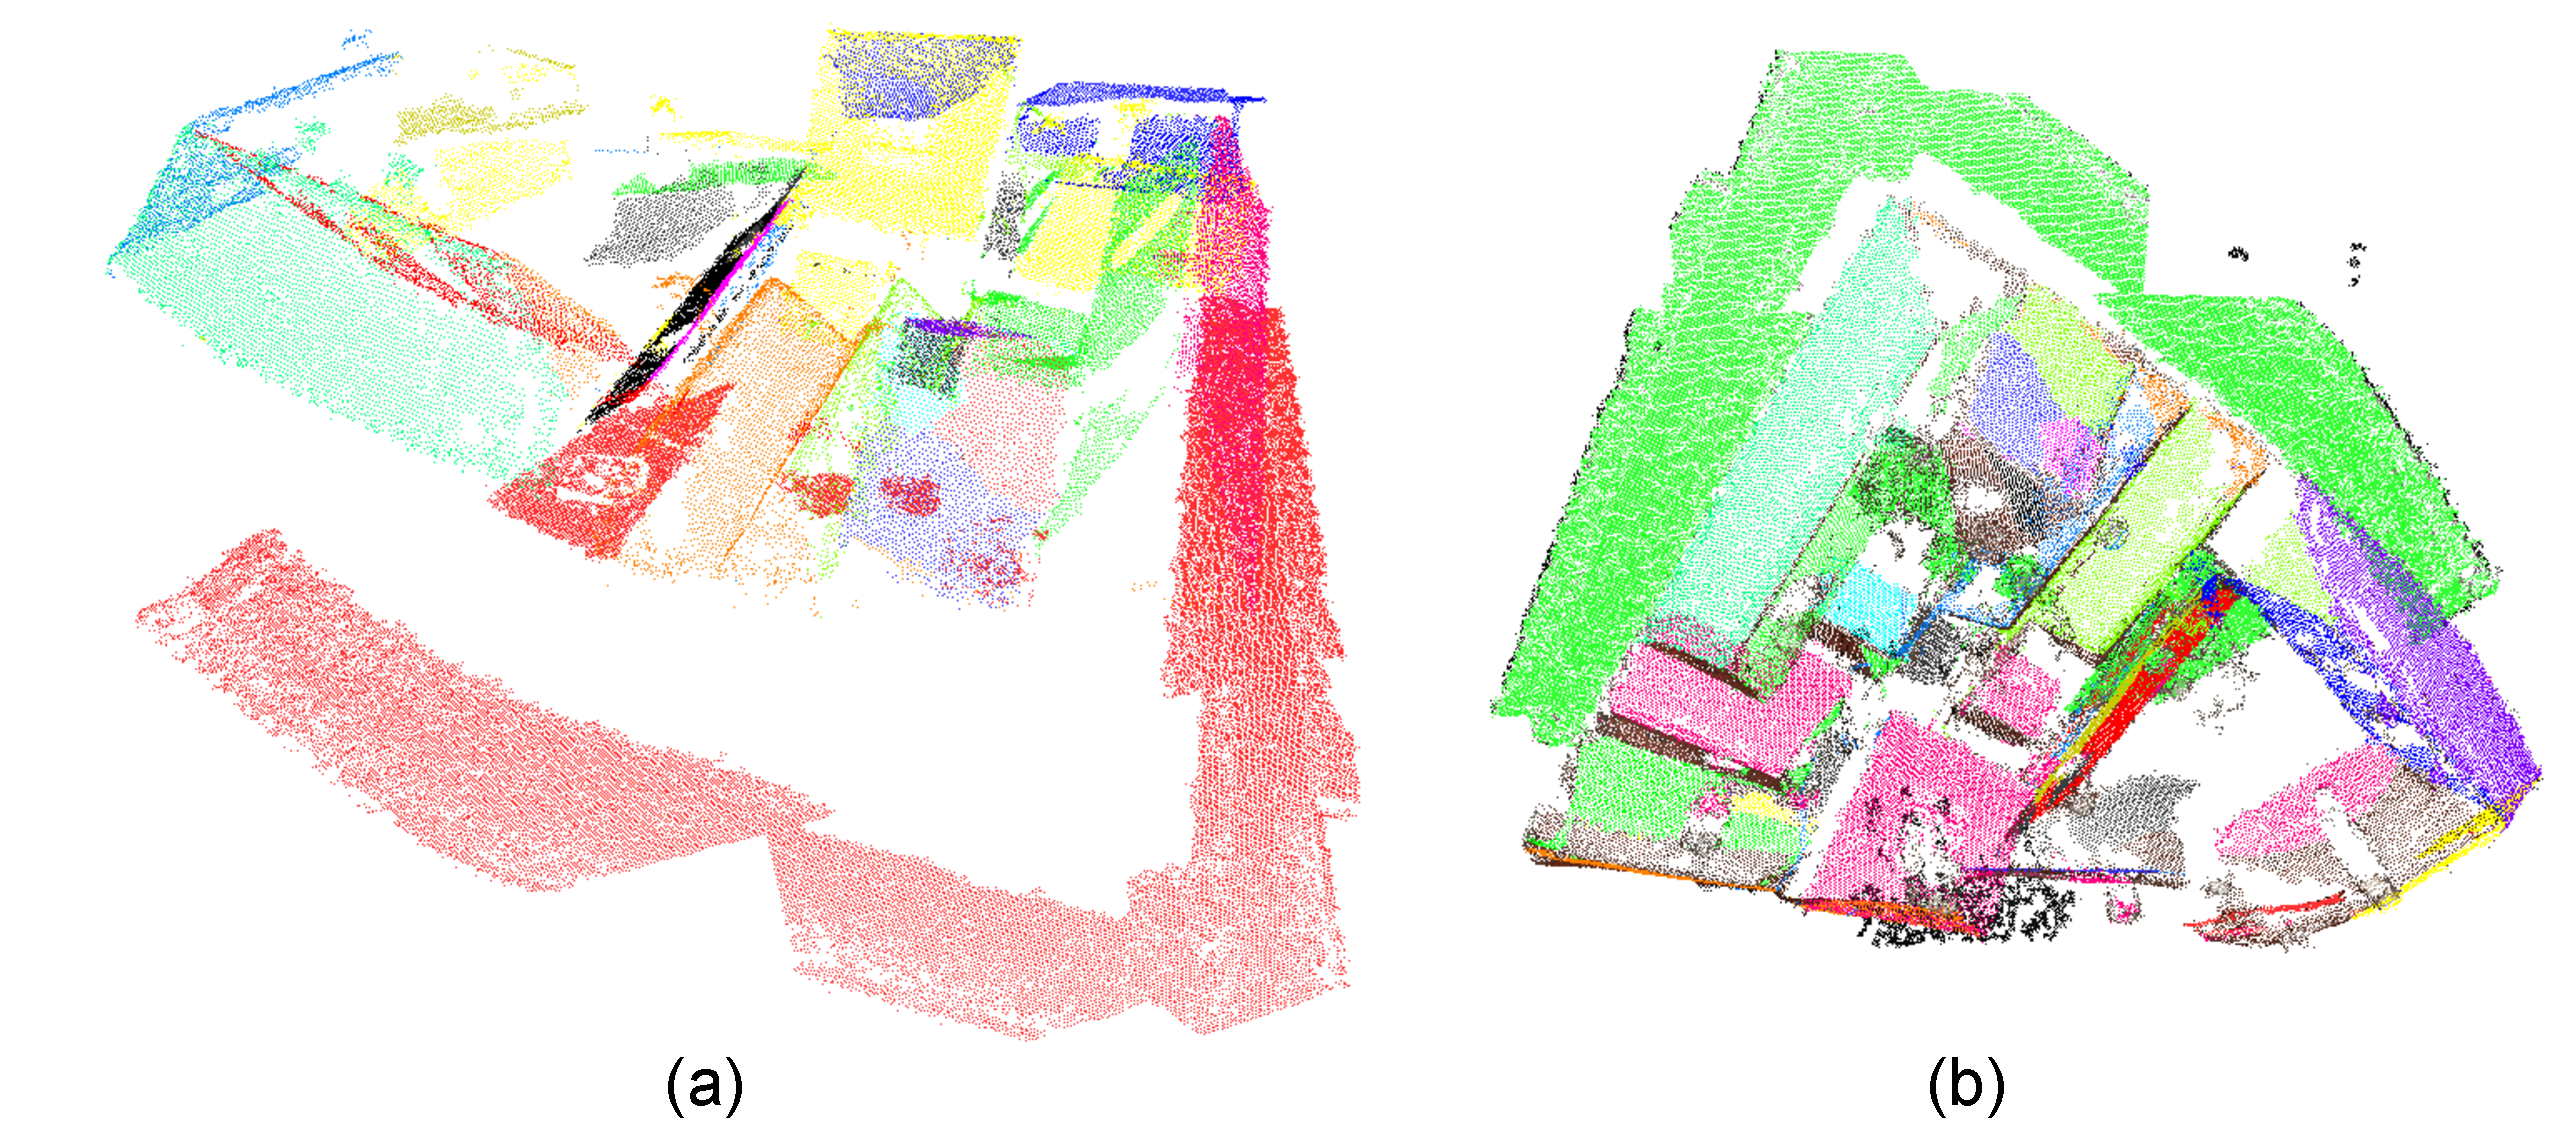
\includegraphics[width=\textwidth]{figures/test-lw}
\caption{Ukázka segmentace mračna Langweil. (a) zobrazuje pouze nalezené segmenty, (b) zobrazuje segmenty včetně bodů, které nebyly segmentovány.}
\label{fig:test-lw}
\end{center}
\end{figure}

Segmentace mračna není určitě tak kvalitní, jak by se dalo očekávat. Problém v tomto případě však není vyloženě v algoritmu segmentace, ale ve vstupních datech. Protože se jedná o sken starého papírového modelu, většina střech není rovná, naopak střechy jsou prohnuté či různě lomené. Segmentace tedy některé střechy nenalezla, protože nejsou rovné, u jiných našla např. dva segmenty na jedné střeše, protože střecha je různě zprohýbaná. Výsledky segmentace tedy nejdou příliš dobře zhodnotit, vstupní mračno není vhodné pro testování planární segmentace.

Jako pokus jsem zvolil malé okolí bodu, hodnotu jsem nastavil na 10. Tím jsem docílil toho, že výpočet parametrů nebyl příliš přesný, identifikované segmenty měly tedy větší RMS a obvykle obsáhly více bodů ze svého okolí. Tím jsem chtěl dosáhnout toho, že když střechny nejsou příliš rovné, horší přesnost vypočtených parametrů by mohla částečně tento problém \uv{zakrýt}. Tato myšlenka se ve skutečnosti ukázala správná a opravdu bylo nalezeno méně segmentů, které více odpovídaly střechám. Pokud jsem při testování používal větší velikost okolí, algoritmus nacházel více segmentů, který byly sice relativně přesnější, ale méně odpovídaly \uv{reálným} rovinám.

Celkově tedy segmentace příliš neodpovídá tomu, co bychom na první pohled očekávali, nicméně minimálně spodní velká rovina byla nalezena, stejně tak několik rovnějších střech bylo identifikováno správně. Algoritmus by tedy neměl mít problém segmentovat menší mračna s menší hustotou bodů.


\newpage
\section{Shrnutí výsledků testování}

V první části testování jsme ověřovali funkčnost algoritmu na uměle generovaných datech. Ve všech těchto testech byly nalezeny všechny roviny a bylo segmentováno více jak 99\% bodů, algoritmus tedy na těchto ideálních datech funguje správně.

Testování segmentace na reálných datech už nebylo tak bezproblémové, jako u generovaných dat. Celkově však algoritmus vždy našel většinu rovin a do segmentu přiřadil většinu bodů z dané roviny. Nicméně ne všechny roviny byly vždy nalezeny. Pokud byla nějaká rovina při segmentaci vynechána, obvykle byla tato rovina výrazně menší, než ostatní nalezené roviny, resp. obsahovala výrazně méně bodů. Problematická se tedy ukázala i situace, kdy měly roviny výrazněji odlišnou hustotu bodů. Roviny s malou hustotu bodů (tedy i malým počtem bodů) často v akumulátorovém poli nevytvořily dostatečně výrazný vrchol a nebyly nalezeny. Dále také nemusejí být nalezené roviny, které na malém měřítku nejsou příliš rovné, naopak jsou různě zvlněné nebo hrbolaté. Do určité míry se dá toto kompenzovat správným nastavením parametrů, někdy ale ani to nestačí. 

Dále jsme při testování také narazili na dva problémy, které se netýkali přímo nalezení segmentů, ale jejich kvality či správnosti. Prvním problémem byla situace, kdy v akumulátorovém poli dvě roviny vytvořily vrcholy těsně vedle sebe a při vyhledávání vrcholů byl nalezen jen jeden. V této situaci mohly být do segmentu přiřazeny body i z druhého vrcholu, tedy z jiné roviny. Taková situace při reálném testování je zobrazena na obrázku \ref{fig:test-do} (b), kde zelený segment střechy obsahuje i body z boční stěny. Druhým problémem byla situace, kdy v nejvyšší buňce z vrcholu v akumulátorovém poli byly velmi přesné body. Segment vytvořený z tohoto vrcholu obsahoval pouze body, které ležely velmi přesně v rovině. V akumulátorovém poli poté zbyly body, které stále ještě ležely v rovině, která akorát nebyla tak přesná. Pokud bylo takových bodů dostatečné množství, při další iteraci prohledávání akumulátorového pole mohly být identifikovány jako segment. Výsledkem tedy byly dva segmenty v jedné rovině. Příklad této situace je zobrazen na obrázku \ref{fig:test-fa}.

V celkovém součtu všech testů\footnote{Není zahrnut poslední test mračna Langweil, které nebylo pro testování příliš vhodné.} mračna obsahovala 85 rovin a algoritmus správně detekoval 68 rovin, což je přesně 80\%. Algoritmus tedy není bezchybný, ale je schopen správně detekovat většinu rovin. Navíc nenalezené roviny jsou vždy menší či méně přesné, nestalo se, aby algoritmus nenašel nějakou výraznou rovinu.

Co se týče paměťových a časových nároků, ty jsou logicky nejvíce závislé zejména na velikosti vstupních dat. Doba běhu algoritmu je navíc závislá na zadaných parametrech, které mohou segmentaci zkvalitnit, vždy ale na úkor delšího běhu algoritmu.


%*****************************************************************************
\chapter{Závěr}

Cílem této práce bylo nastudovat, implementovat a otestovat dva zadané algoritmy. V průběhu práce na prvním algoritmu jsem bohužel zjistil, že pochopení a následná implementace algoritmu bude náročnější, než jsem předem očekával. To bylo způsobené částečně tím, že tato práce byla moje první seznámení s 3D rekonstrukcí mračen bodů, obecně byla i mojí první větší zkušenosté se zpracováním takto velkých vstupních dat. Z těchto důvodů jsem strávil přiliš mnoho času při studování základních principů a technik. V neposlední řadě jsem se dlouhou dobu učil debuggovat takovýto druh algoritmu, což není jednoduché, protože veškerá zpracoávaná data mají pouze matematické vyjádření (body, roviny), které se nedá jednoduše představit a vzhledem k množství vstupních dat se často nedá ani jednoduše vykreslit. Z těchto důvodů jsem se s vedoucím práce dohodl, že zpracuji pouze první (a také složitější) algoritmus, oba algoritmy bych bohužel zpracovat nestihl. Nicméně nemyslím si, že by celkový rozsah práce byl nedostatečný. Tím, že jsem implementoval pouze jeden algoritmus, jsem se na něj mohl více zaměřit a také jsem mohl více času věnovat testování, aby byl algoritmus co nejkvalitnější na reálných datech.

Co se týče zpracovaného algoritmu, i když byl teoreticky popsán velmi podrobně, jeho implementace vyžadovala mnoho vlastních úprav a myšlenek. Předně bylo důležité zvolit vhodné datové struktury pro reprezentaci mračna bodů a pro správnou reprezentaci akumulátorového pole. Dále bylo nutné vyhledat knihovny pro reprezentaci kd-stromu a SVD dekompozici s důrazem na co nejvyšší výkon. Než jsem nalezl knihovny, které jsem ve výsledku použil, testoval jsem desítky různých více či méně kvalitních řešení. Při testování těchto knihoven mně osobně překvapilo, že i když mají dané metody ve všech knihovnách stejnou asymptotickou složitost, výsledný reálný výkon těchto knihoven byl velmi závislý na zvolené implementace a mezi jednotlivými knihovnami se výrazně lišil.

Dále jsem se při implementaci algoritmu musel vypořádat se skutečností, že autoři původního článku používali pro testování odlišný typ vstupních dat s definovaným šumem (odchylkou bodů v daných směrech), na jehož základě odvozovali mnohé rozměry a hodnoty. Já jsem takovýto šum v datech neměl definovaný, proto jsem musel vymyslet vlastní definice pro výpočet velikosti okolí, velikosti bufferu při definici okolí, velikosti akumulátorového pole apod. Dále jsem upravil metodu pro vybírání bodů z akumulátorového pole, kdy jsem místo vybírání vrcholů po jednom navrhl vybírání všech vrcholů postupně, čímž jsem předešl nežádoucím chybám v situaci, kdy byly dva vrcholy v akumulátorovém poli v těsné blízkosti. V neposlední řadě jsem implementaci rozdělil na dvě nezávislé části, které je možné provádět odděleně, tím je dána uživateli možnost provádět jednu část algoritmu opakovaně bez nutnosti provádět celý algoritmus, čímž lze výrazně ušetřit výsledný čas strávený segmentací. Nakonec jsem také definoval tři parametry, které uživateli umožní přizpůsobit kvalitu a rychlost segmentace na konkrétní zpracovávaná data. Toto je sice na úkor automatizace celého algoritmu, nicméně nedovedu si představit, že by takovýto algoritmus fungoval plně automaticky na naprosto různých vstupních datech.

Algoritmus ale samozřejmě není dokonalý, testování ukázalo několik problematických situací, kdy segmenty nebyly nalezeny nebo naopak byly nalezeny dva segmenty v rámci jedné roviny. Zde je rozhodně prostor pro případné rozšíření práce nebo navázání na práci. Je zde prostor pro definování lepší metody určení velikosti akumulátorového pole, určitě by také bylo možné vylepšit metodu vyhledávání vrcholů v akumulátorovém poli a jejich následné vybírání. Vylepšení těchto částí algoritmu by se mohlo výrazně projevit na zlepšené kvalitě segmentace, která by byla schopna detekovat větší množství segmentů. Je však nutné vzít v úvahu, že zde jsou omezení dané samotným principem hlasování do akumulátorového pole. Nedá se očekávat, že by byl algoritmus schopný nalézt roviny o desítkách až stovkách bodů v mračnech, které obsahují statisíce až miliony bodů s nezanedbatelným množstvím šumu a bodů, které v žádných rovinách neleží. Dále je zde také možnost zjednodušit či vylepšit systém zadávaných parametrů, případně nějaký parametr efektivně odebrat. Každý takováto povinný uživatelský parametr výrazně snižuje použitelnost algoritmu, uživatel je nyní nucen pochopit alespoň základní princip algoritmu, aby byl schopen parametryvhodně zvolit.

Pokud bych měl celkově zhodnotit kvalitu algoritmu, tak si myslím, že algoritmus je poměrně efektivní a je schopen ve velmi různorodých mračnech bodů nalézt většinu požadovaných rovin v přijatelné kvalitě, ale rozhodně zde je prostor pro vylepšení.




%*****************************************************************************
% Seznam literatury je v samostatnem souboru reference.bib. Ten
% upravte dle vlastnich potreb, potom zpracujte (a do textu
% zapracujte) pomoci prikazu bibtex a nasledne pdflatex (nebo
% latex). Druhy z nich alespon 2x, aby se poresily odkazy.

% originally following specification for bibliography formating was used
%\bibliographystyle{abbrv}

% Here is an improvment by Petr Dlouhy (April 2010).
% It is mainly for supervisors who expect Czech fomrating rules for references
% Additional feature is live url addresses to sources from your pdf file
% It requires the file csplainnat.bst (included in this sample zipfile).

\bibliographystyle{csplainnat}

%bibliographystyle{plain}
%\bibliographystyle{psc}
%{
%JZ: 11.12.2008 Kdo chce mit v techto ukazkovych odkazech take odkaz na CSTeX:
\def\CS{$\cal C\kern-0.1667em\lower.5ex\hbox{$\cal S$}\kern-0.075em $}
\bibliography{reference}
%}

% M. Dušek radi:
%\bibliographystyle{alpha}
% kdy citace ma tvar [AutorRok] (napriklad [Cook97]). Sice to asi neni podle ceske normy (BTW BibTeX stejne
% neodpovida ceske norme), ale je to nejprehlednejsi.
% 3.5.2009 JZ polemizuje: BibTeX neobvinujte, napiste a poskytnete nam styl (.bst) splnujici citacni normu
% CSN/ISO.

%*****************************************************************************
%*****************************************************************************
\appendix

%*****************************************************************************
\chapter{Seznam použitých zkratek}
\label{chap:zkratky}

\begin{description}
\item[RMS] Root Mean Square, česky efektivní hodnota. Určuje velikost měnící se veličiny.
\item[P1] Parametr, který určuje velikost okolí bodu.
\item[P2] Parametr klastrování, který určuje práh vyhledávání vrcholů v akumulátorovém poli.
\item[P3] Parametr, který určuje kvalitu klastrování.
\end{description}


%*****************************************************************************
\chapter{Instalační a uživatelská příručka}
Tady asi nemám moc co psát\ldots


%*****************************************************************************
\chapter{Obsah přiloženého CD}
\label{chap:CD}
Tato příloha je povinná pro každou práci. Každá práce musí totiž obsahovat přiložené CD. Viz dále.

Může vypadat například takto. Váš seznam samozřejmě bude odpovídat typu vaší práce.

%\begin{figure}[h]
%\begin{center}
%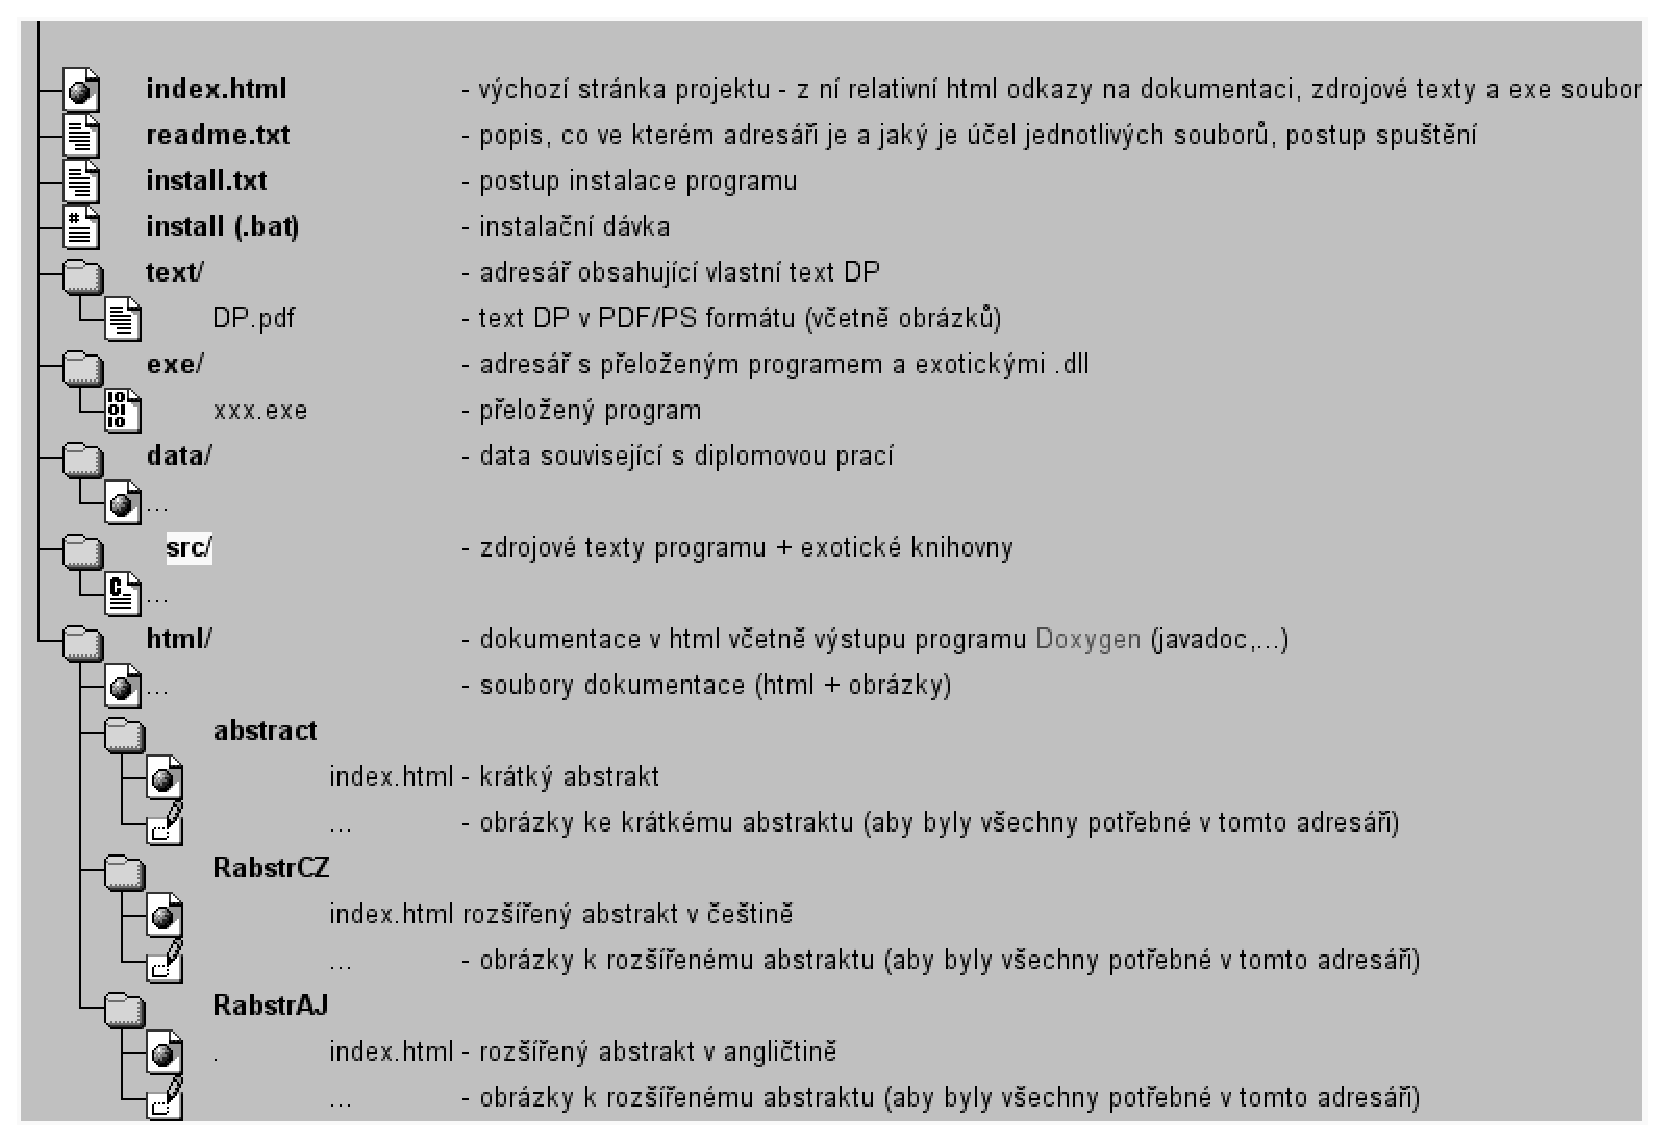
\includegraphics[width=14cm]{figures/seznamcd}
%\caption{Seznam přiloženého CD --- příklad}
%\label{fig:seznamcd}
%\end{center}
%\end{figure}

Na GNU/Linuxu si strukturu přiloženého CD můžete snadno vyrobit příkazem:\\ 
\verb|$ tree . >tree.txt|\\
Ve vzniklém souboru pak stačí pouze doplnit komentáře.

Z \textbf{README.TXT} (případne index.html apod.)  musí být rovněž zřejmé, jak programy instalovat, spouštět a
jaké požadavky mají tyto programy na hardware.

Adresář \textbf{text}  musí obsahovat soubor s vlastním textem práce v PDF nebo PS formátu, který bude později
použit pro prezentaci diplomové práce na WWW.

\end{document}
